%!TEX root = Manuscrit.tex
\chapter{Cartographie automatisée d'images aériennes}
\label{chap:cartographie}
	%\citationChap{Et la géographie, c'est exact, m'a beaucoup servi. Je savais reconnaître, du premier coup d'oeil, la Chine de l'Arizona. C'est très utile, si l'on est égaré pendant la nuit.}{Saint-Exupéry (Le Petit Prince, 1943)}
	\minitoc

%%%%%%%%%%%%%%%%%%%%%%%%%%%%%%%%%%%%%%%%%%%%%%%%%%%%%%%%%%%%%%%%%%%%%%%%%%%%%%%%%%%%%%%%%%%%%
\chapsummary{%
	Ce chapitre présente deux méthodes pour la segmentation sémantique d'images aériennes très haute résolution : la classification par région et les réseaux entièrement convolutifs.

	La classification par région consiste à découper l'image en régions homogènes via un algorithme de segmentation non-supervisé. Les régions ainsi obtenues sont ensuite classifiées une à une. Nous étudions plus particulièrement l'utilisation de caractéristiques profondes issues de \glsname{CNN} pré-entraînés. Nous montrons notamment que les caractéristiques profondes de réseaux entraînés sur des images multimédia peuvent se transférer avec succès pour l'analyse d'images aériennes.

	Par ailleurs, nous identifions les propriétés souhaitables des segmentations non-supervisées dans le processus de classification par région. Nous mettons en exergue leur rôle limitant, les imprécision et la sous-résolution des segmentations ne pouvant être compensé que par une diminution de la taille des régions, coûteuse en temps de calcul. Nous étudions ainsi des approches par réseaux de neurones entièrement convolutifs, capables de réaliser une extraction de caractéristiques et une classification dense sur tous les pixels d'une image en une seule inférence.

	Nous adaptons plusieurs modèles de l'état de l'art pour la segmentation sémantique d'images naturelles au traitement de données de télédétection, sur lesquelles nous montrons la supériorité empirique des tels réseaux entièrement convolutifs par rapport aux méthodes de classification usuelles. Nous étudions en outre plusieurs variantes permettant de prendre en compte différents niveaux de contexte spatial pour une meilleure précision.
}
\newpage

\section{Classification par région d'images aériennes}

\begin{figure}[t]
	\resizebox{\textwidth}{!}{\documentclass{standalone}
\usepackage[utf8]{inputenc}
\usepackage[T1]{fontenc}
\usepackage{tikz}
%%%%%%%%%%%%%%%%%%%%%%%%%%%%%%%%%%%%%%%%
%           Commandes perso            %
%%%%%%%%%%%%%%%%%%%%%%%%%%%%%%%%%%%%%%%%

%% Figures centrées, et en position 'here, top, bottom or page'
\newenvironment{figureth}{%
		\begin{figure}[htbp]
			\centering
	}{
		\end{figure}
		}


%% Tableaux centrés, et en position 'here, top, bottom or page'
\newenvironment{tableth}{%
		\begin{table}[htbp]
			\centering
			%\rowcolors{1}{coleurtableau}{coleurtableau}
	}{
		\end{table}
		}

%% Sous-figures centrées, en position 'top'
\newenvironment{subfigureth}[1]{%
	\begin{subfigure}[t]{#1}
	\centering
}{
	\end{subfigure}
}

\newcommand{\citationChap}[2]{%
	\epigraph{\og \textit{#1} \fg{}}{#2}
}

%% On commence par une page impaire quand on change le style de numérotation de pages
\let\oldpagenumbering\pagenumbering
\renewcommand{\pagenumbering}[1]{%
	\cleardoublepage
	\oldpagenumbering{#1}
}

%% Légende du dataset ISPRS
\newcommand\isprslegende{
Légende\,: \textcolor{Black}{blanc}\,: routes, \textcolor{Blue}{bleu}\,: bâtiments, \textcolor{Cerulean}{cyan}\,: végétation basse, \textcolor{OliveGreen}{vert}\,: arbres, \textcolor{Dandelion}{jaune}\,: véhicules, \textcolor{BrickRed}{rouge}\,: autre.
}

%% Dessiner des réseaux de neurones avec Tikz
\newcommand{\convlayer}[9]{%{h}{w}{d}{name}{color}{x}{y}{z}%{note w}{note h}{note d}
   \def\h{#1}
   \def\w{#2}
   \def\d{#3}
   \def\name{#4}
   \ifthenelse {\equal{#5} {}} {\def\col{white}} {\def\col{#5}}
   \def\x{#6}
   \ifthenelse {\equal{#7} {}} {\def\y{0}} {\def\y{#7}}
   \ifthenelse {\equal{#8} {}} {\def\z{0}} {\def\z{#8}}
   % ne faites pas ça chez vous !
   \ifthenelse {\equal{#9} {}} {\convlayercontinued{}{}{}} {\convlayercontinued#9}
}

\newcommand\convlayercontinued[3]{
   \def\notew{#1}
   \def\noteh{#2}
   \def\noted{#3}
   \coordinate (A) at (\x-\d/2,  \y-\h/2, \z-\w/2);
   \coordinate (B) at (\x-\d/2,  \y-\h/2, \z+\w/2);
   \coordinate (C) at (\x-\d/2,  \y+\h/2, \z+\w/2);
   \coordinate (D) at (\x-\d/2,  \y+\h/2, \z-\w/2);
   \coordinate (E) at (\x+\d/2,  \y-\h/2, \z-\w/2);
   \coordinate (F) at (\x+\d/2,  \y-\h/2, \z+\w/2);
   \coordinate (G) at (\x+\d/2,  \y+\h/2, \z+\w/2);
   \coordinate (H) at (\x+\d/2,  \y+\h/2, \z-\w/2);

    \draw [draw opacity=0.3, fill opacity=0.8, fill=\col!60!white] (A) -- (B) -- (C) -- (D) -- cycle;
    \draw [draw opacity=0.3, fill opacity=0.8, fill=\col!60!white] (A) -- (B) -- (F) -- (E) -- cycle;
    % Face haut
    %\draw [left color=\col!60!white, right color=\col!80!white, shading=axis, shading angle=180] (C) -- (D)  -- (H) -- (G) -- cycle;
    \draw [fill opacity=0.9, fill=\col!70!white] (C) -- node[rotate=45,above] {\small \name} (D) -- (H) -- (G) -- cycle;
    %\draw [fill opacity=0.9, fill=\col!70!white] (C) -- (D) -- node[above] {\small \name} (H) -- (G) -- cycle;
    % Face droite
    \draw [fill opacity=0.9, fill=\col!60!white] (E) -- node[pos=0.75,rotate=45,below] {\scriptsize \notew} (F) -- (G) --  (H) -- cycle;
    % Face avant
    %\draw [shading=axis, left color=\col!60!white, right color=\col!40!white, shading angle=-45] (B) -- node[above,rotate=90] {\scriptsize \noteh} (C) -- (G) -- (F) -- node[below] {\scriptsize \noted}  cycle;
    \draw [fill opacity=0.9, fill=\col!50!white] (B) -- node[above,rotate=90] {\scriptsize \noteh} (C) -- (G) -- (F) -- node[below] {\scriptsize \noted}  cycle;
}

\newcommand{\fclayer}[8]{%{h}{w}{name}{color}{x}{y}{z}
   \def\h{#1}
   \def\w{#2}
   \def\name{#3}
   \ifthenelse {\equal{#4} {}} {\def\col{white}} {\def\col{#4}}
   \def\x{#5}
   \def\y{#6}
   \def\z{#7}
   \def\note{#8}
   \coordinate (A) at (\x-\w/2,  \y-\h/2, \z);
   \coordinate (B) at (\x+\w/2,  \y-\h/2, \z);
   \coordinate (C) at (\x+\w/2,  \y+\h/2, \z);
   \coordinate (D) at (\x-\w/2,  \y+\h/2, \z);

   \pgfmathparse{4*\w}\let\boxwidth\pgfmathresult
    \draw [fill=\col] (A) -- node[below,text width=\boxwidth cm,align=center] {\scriptsize \note} (B) -- (C) -- (D) -- cycle;

    \node (N) at ($(A)!0.5!(B)+(0,-1,0)$) {\name};
}

\newcommand{\alexnet}[4]{%{scale}{x}{y}{z}
  \def\scale{#1}
  \def\alexx{#2}
  \def\alexy{#3}
  \def\alexz{#4}


  \def\coblue{blue!50!white}
  \def\fcgrey{gray!50!white}

  \convlayer{1.3*\scale}{1.3*\scale}{0.02*\scale}{Image}{\coblue}{\alexx}{\alexy}{\alexz}{{227}{227}{3}}
  \convlayer{1.1*\scale}{1.1*\scale}{0.08*\scale}{Conv1}{\coblue}{\alexx+0.7*\scale}{\alexy}{\alexz}{{55}{55}{96}}
  \convlayer{0.7*\scale}{0.7*\scale}{0.5*\scale}{Conv2}{\coblue}{\alexx+1.5*\scale}{\alexy}{\alexz}{{27}{27}{256}}
  \convlayer{0.5*\scale}{0.5*\scale}{0.8*\scale}{Conv3}{\coblue}{\alexx+2.6*\scale}{\alexy}{\alexz}{{13}{13}{384}}
  \convlayer{0.5*\scale}{0.5*\scale}{0.8*\scale}{Conv4}{\coblue}{\alexx+3.8*\scale}{\alexy}{\alexz}{{13}{13}{384}}
  \convlayer{0.5*\scale}{0.5*\scale}{0.5*\scale}{Conv5}{\coblue}{\alexx+4.8*\scale}{\alexy}{\alexz}{{13}{13}{256}}
  \fclayer{\scale}{0.1*\scale}{FC1}{\fcgrey}{\alexx+5.4*\scale}{\alexy}{\alexz}{4096}
  \fclayer{\scale}{0.1*\scale}{FC2}{\fcgrey}{\alexx+5.7*\scale}{\alexy}{\alexz}{4096}
  \fclayer{\scale}{0.1*\scale}{FC3}{\fcgrey}{\alexx+6.0*\scale}{\alexy}{\alexz}{1000}
}

\newcommand{\imagelayer}[7]{%{width}{x}{y}{z}{path}{text_up}{text_down}
    \pgfmathparse{#1}\let\w\pgfmathresult
    \begin{scope}[canvas is yz plane at x=#2]
     \node[transform shape] (source) at (#3, #4) {\includegraphics[angle=-90,width=\w cm]{#5}};
    \end{scope}
     \node [transform shape, rotate=45, above] at (source.east) {#6};
     \node [transform shape, rotate=45, below] at (source.west) {\scriptsize{#7}};
}

\def\fourier{\mathcal{F}}

\newcommand{\lightspectrum}{%
\pgfplotsset{
    % this *defines* a custom colormap ...
    colormap={slategraywhite}{color(0cm)=(red); color(1cm)=(red); color(2cm)=(red); color(3cm)=(red); color(4cm)=(orange); color(5cm)=(yellow); color(6cm)=(green); color(7cm)=(blue); color(8cm)=(blue); color(9cm)=(purple); color(10cm)=(purple); color(12cm)=(black)}
}
\node at (1.5, 2.7) {\small 1mm};
\node at (4, 3) {Infrarouge};
\node at (7.75, 2.7) {\small 800nm};
\node at (9, 3) {Visible};
\node at (10.5, 2.7) {\small 400nm};
\node at (12, 3) {Ultraviolet};
\node at (13.5, 2.7) {\small 10nm};
\draw[->] (1, 2.5) -- (14, 2.5);
\begin{axis}[hide axis,width=16cm,height=4cm,colormap name=slategraywhite]
\addplot[domain=20:1000,samples=1500,ultra thick, point meta=x*x,mesh]{sin(x*x/80)};
\end{axis}
}

% Union généralisée
\newcommand{\wbigcup}{\mathop{\bigcup}\displaylimits}

\newcommand{\res}[2]{#1 {\footnotesize $\pm$ #2}}
\newcommand{\bres}[2]{\textbf{#1} {\footnotesize $\pm$ #2}}
\newcommand{\bbres}[2]{\res{\textit{#1}}{#2}}

\newcommand{\drawkernel}[9]{
\begin{tikzpicture}
	\draw[step=1cm,gray!50!white,very thin] (0,0) grid (3,3);
	\kernelnode{0.5}{0.5}{#1};
	\kernelnode{0.5}{1.5}{#2};
	\kernelnode{0.5}{2.5}{#3};
	\kernelnode{1.5}{0.5}{#4};
	\kernelnode{1.5}{1.5}{#5};
	\kernelnode{1.5}{2.5}{#6};
	\kernelnode{2.5}{0.5}{#7};
	\kernelnode{2.5}{1.5}{#8};
	\kernelnode{2.5}{2.5}{#9};
\end{tikzpicture}
}

\newcommand{\kernelnode}[3]{%{x}{y}{value}
	\ifthenelse{\equal{#3}{0}}{
		\def\kcolor{gray}
	}{
		\def\kcolor{black}
	}
	\node[\kcolor] at (#1, #2) {#3};
}

\newcommand{\chapsummary}[1]{
\section*{Résumé du chapitre :}
\parbox{0.9\linewidth}{
\setlength{\parindent}{4ex}
#1}
}

\newcommand{\eqname}[1]{\tag*{\small (#1)}}

\begin{document}

\begin{tikzpicture}[every node/.style={inner sep=0,outer sep=0}]
\usetikzlibrary{calc}

\definecolor{colred}{RGB}{211,57,57}
\definecolor{colblue}{RGB}{83,210,246}
\definecolor{colgreen}{RGB}{90,225,79}
\definecolor{colgray}{RGB}{233,232, 198}

\newcommand{\gearmacro}[5]{%
\foreach \i in {1,...,#1} {%
  [rotate=(\i-1)*360/#1]  (0:#2)  arc (0:#4:#2) {[rounded corners=1.5pt]
             -- (#4+#5:#3)  arc (#4+#5:360/#1-#5:#3)} --  (360/#1:#2)
}}  

\node (image) at (0,0) {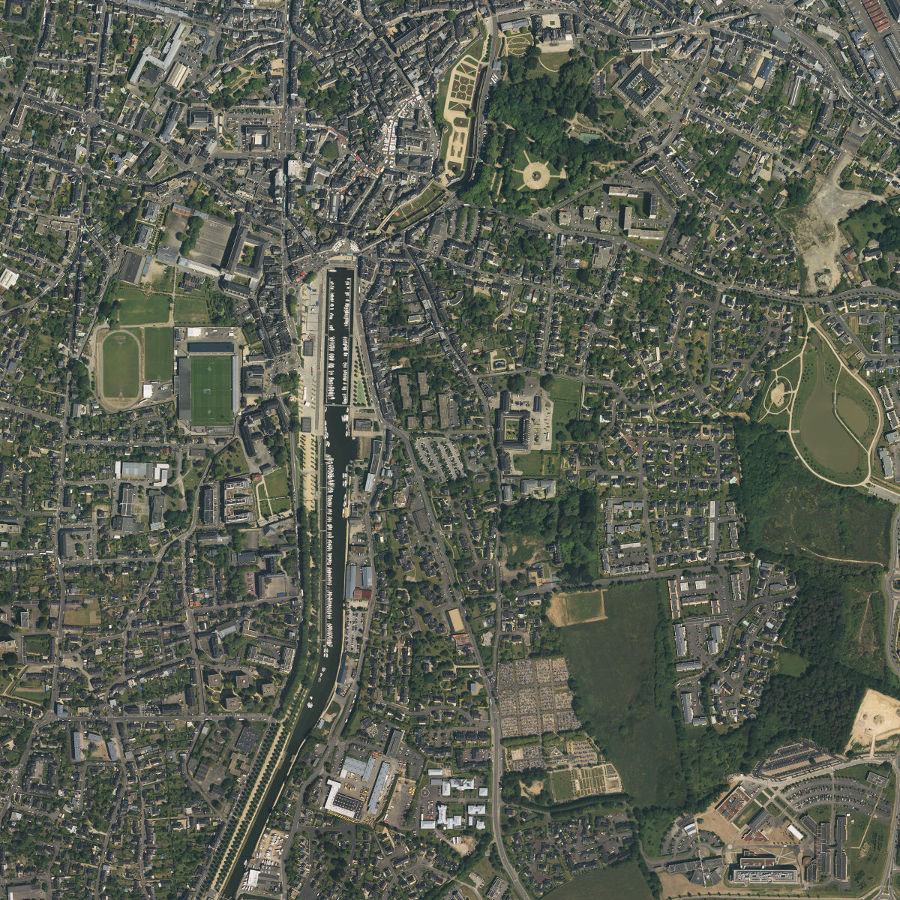
\includegraphics[width=4cm]{ortho.jpg}};

\node (port) at (3.5, 0) {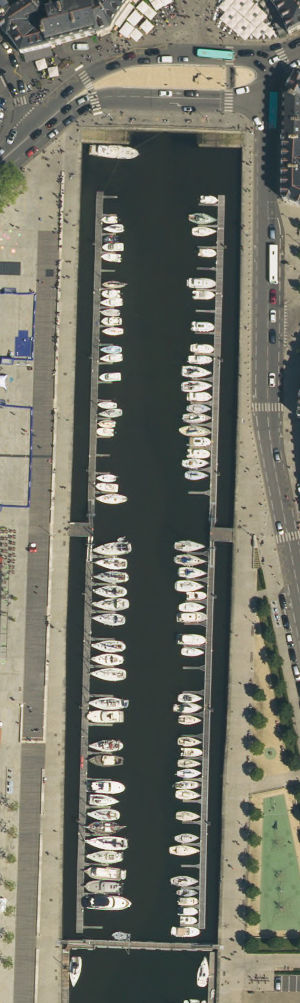
\includegraphics[width=1cm]{port.jpg}};
\node (ubs) at (5.5, -1) {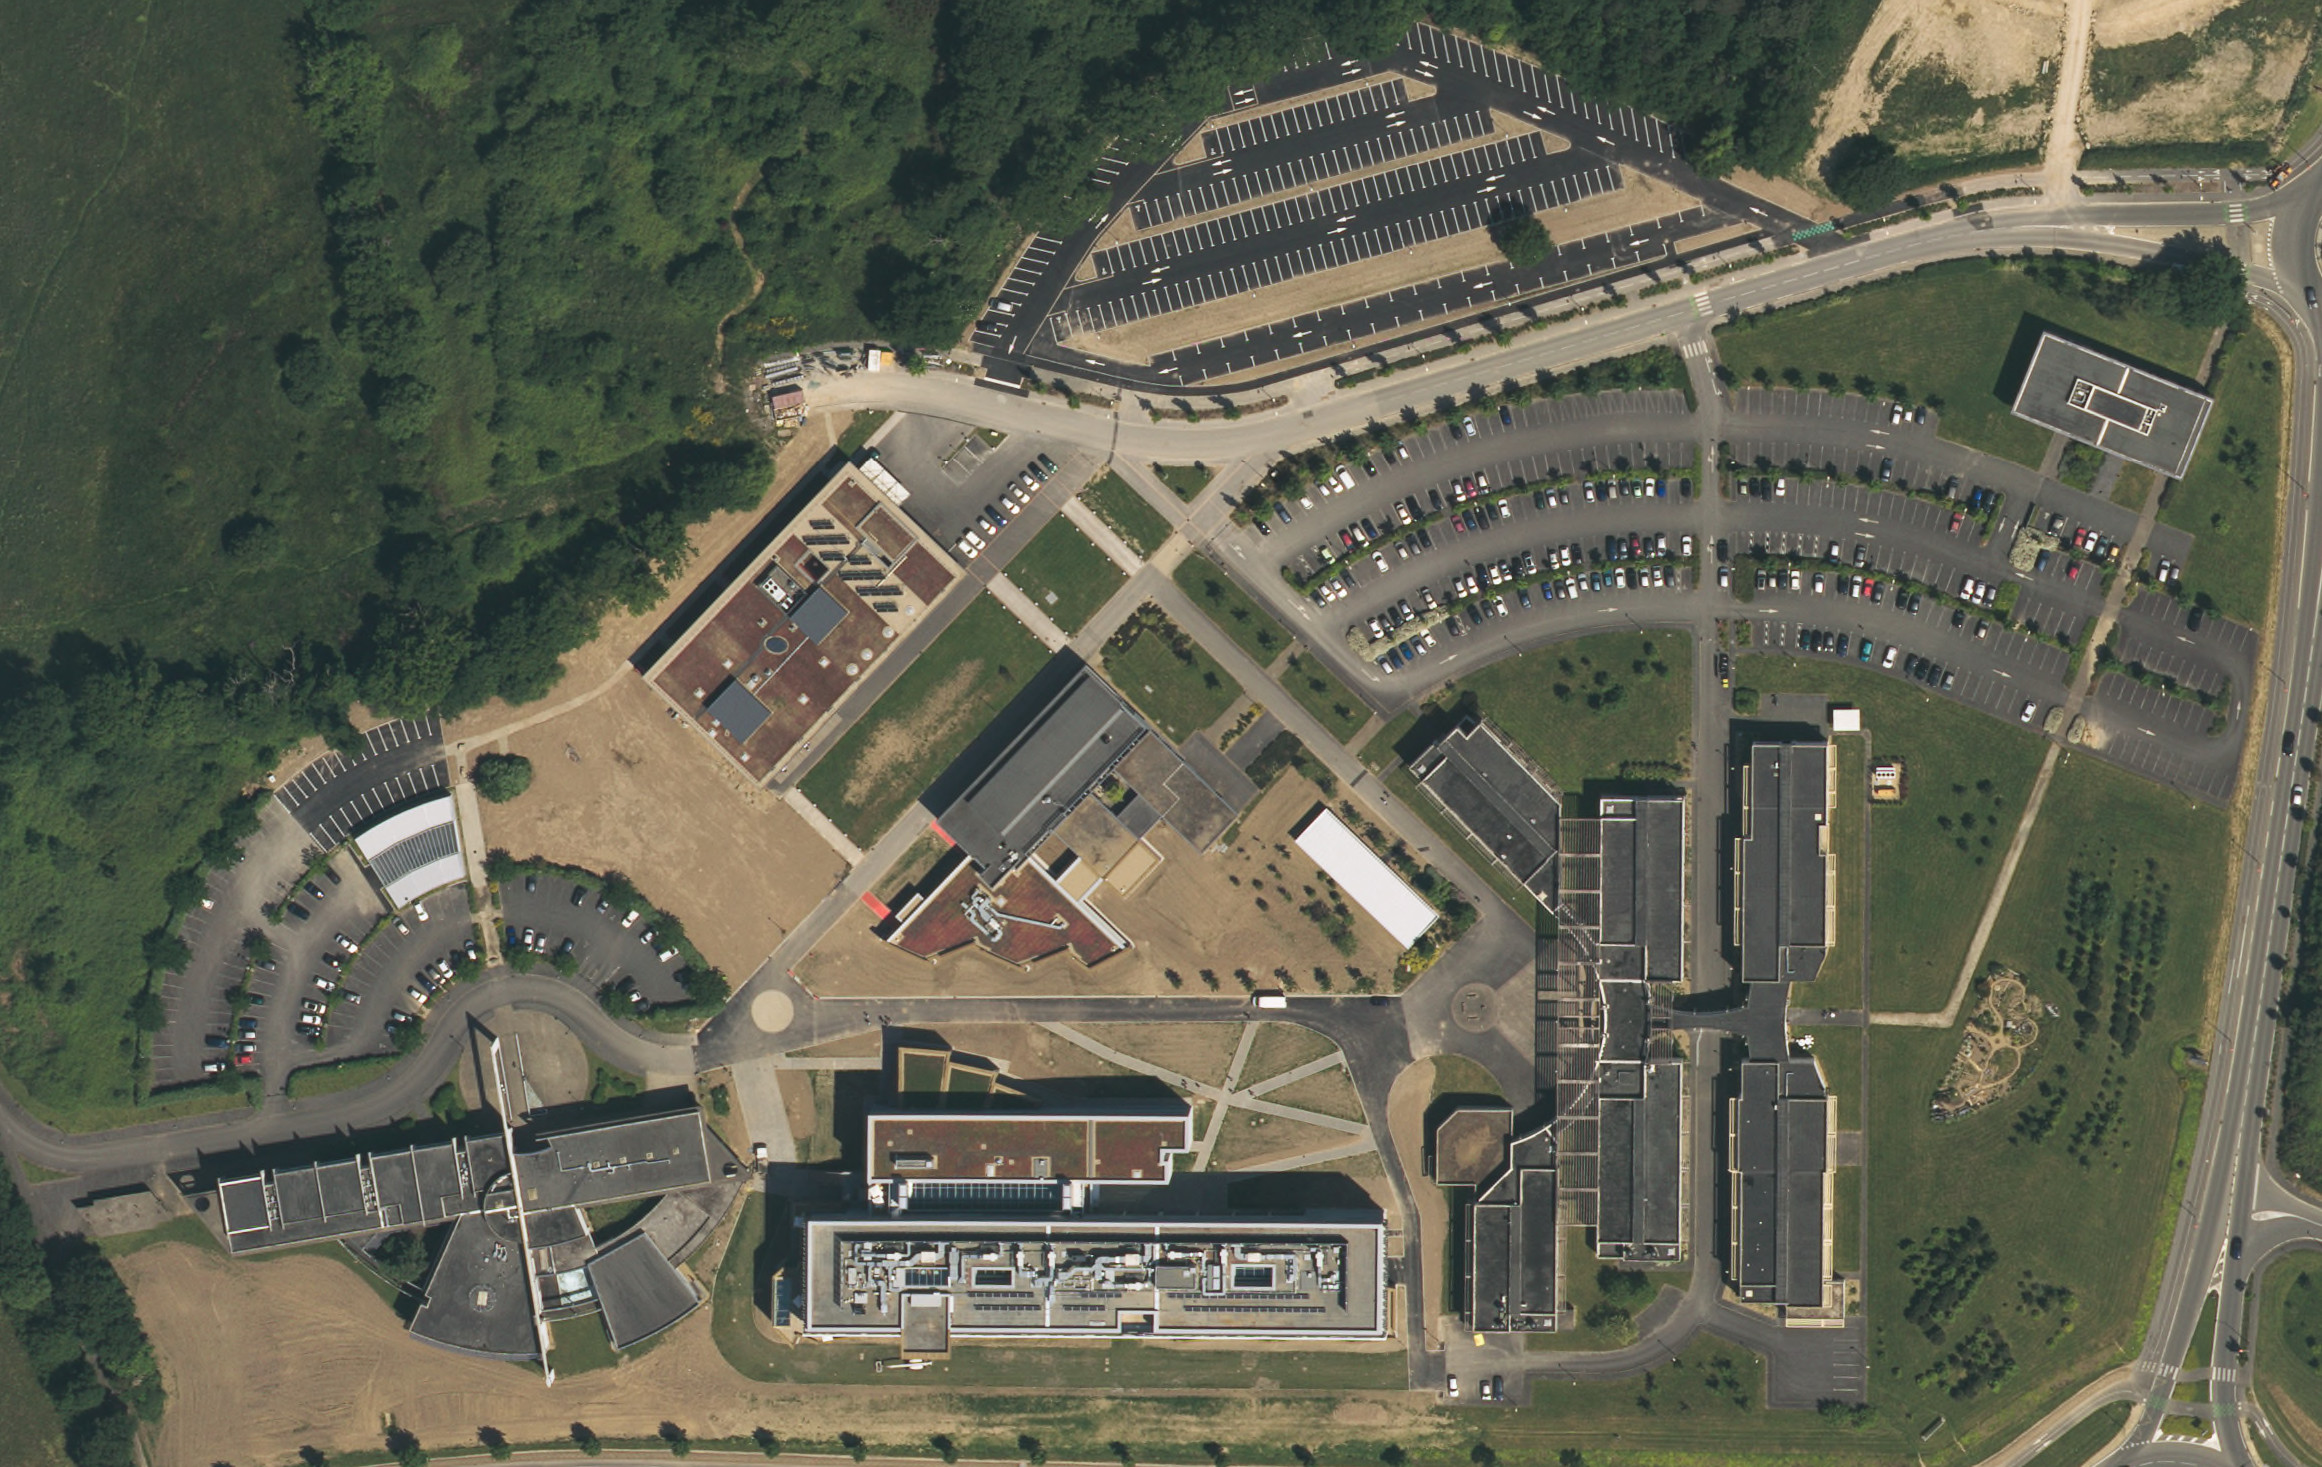
\includegraphics[width=2.5cm]{ubs.jpg}};
\node (jardins) at (5.5, 1.2) {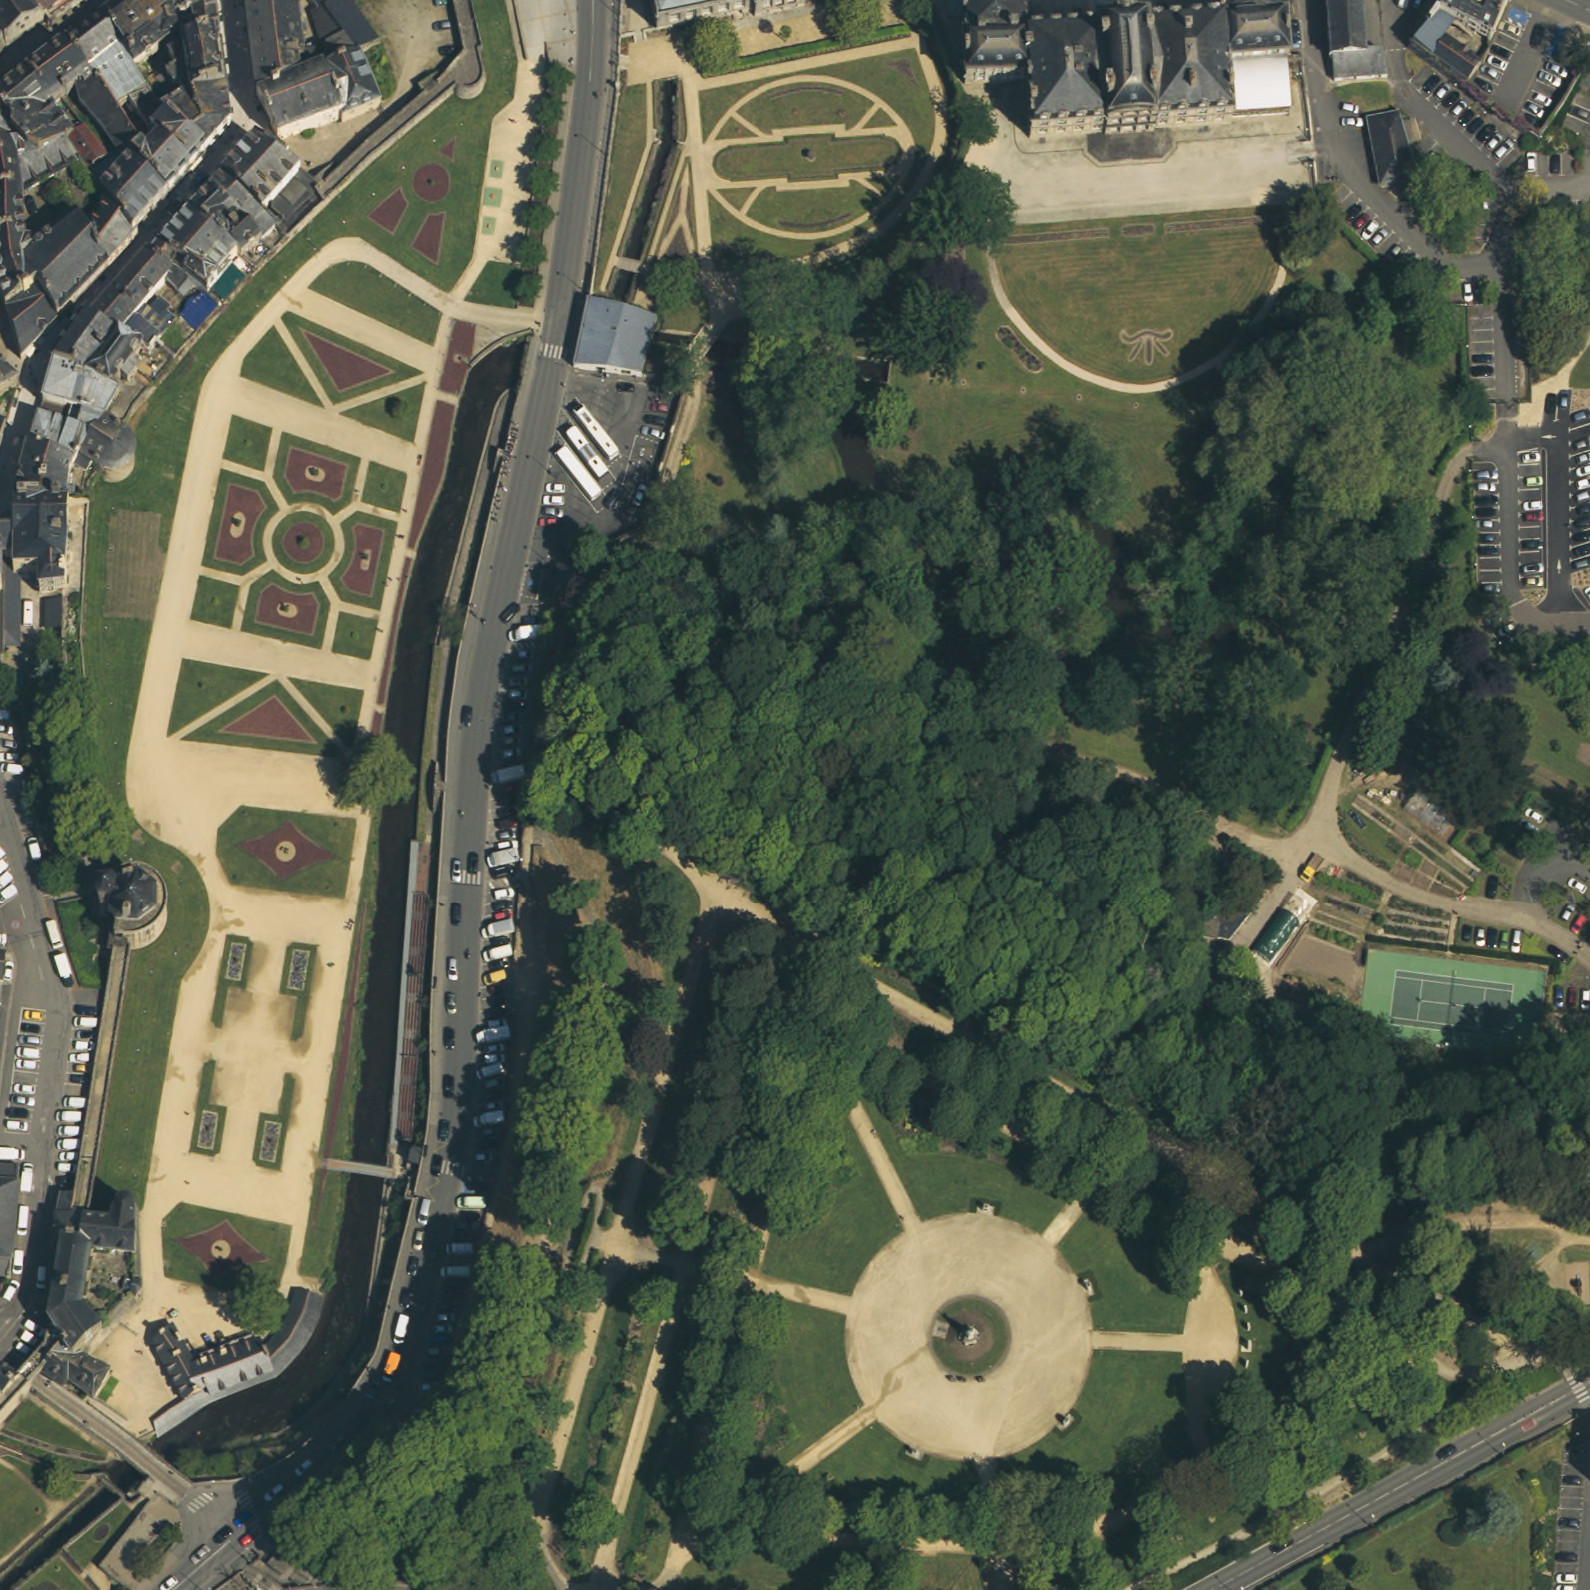
\includegraphics[width=2cm]{jardins.jpg}};


\fill[draw=black,fill=colgray] (7.8,2) rectangle node[yshift=-0.6cm,rotate=90] {Interprétation} (9.2,-2);
\node (interp) at (7.8,0) {};
\node (interpout) at (9.2,0) {};

\node[colblue,draw,line width=0.5mm,minimum width=0.2cm,minimum height=1cm] (portinimage) at ($(image.west)+(1.5,0.5)$) {};
\node[colred,draw,line width=0.5mm,minimum width=1cm,minimum height=0.7cm] (ubsinimage) at ($(image.south)+(1.5,0.35)$) {};
\node[colgreen,draw,line width=0.5mm,minimum width=0.7cm,minimum height=0.5cm] (jardinsinimage) at ($(image.north)+(0.25,-0.7)$) {};

\begin{scope}[shift={(8.5*5,1.2*5)},transform canvas={scale=0.2}]
   \fill[gray] (0,0) circle (2cm);
   \draw[thick,rotate=12,fill=gray] \gearmacro{8}{2}{2.4}{20}{4};
   \draw[thick,fill=colgray] (0,0) circle(1.35);
\end{scope}

\draw (portinimage.east) edge[->,thick,colblue,out=0,in=180,looseness=1] (port.west);
\draw (ubsinimage.south) edge[->,thick,colred,out=-90,in=-90,looseness=0.5] (ubs.south);
\draw (jardinsinimage.north) edge[->,thick,colgreen,out=90,in=90,looseness=0.5] (jardins.north);

\draw (port.east) edge[->,thick,colblue] (interp);
\draw (ubs.east) edge[->,colred,thick] ($(interp)+(0,-0.5)$);
\draw (jardins.east) edge[->,colgreen,thick] ($(interp)+(0,0.5)$);

\node (ua) at (13, 0) {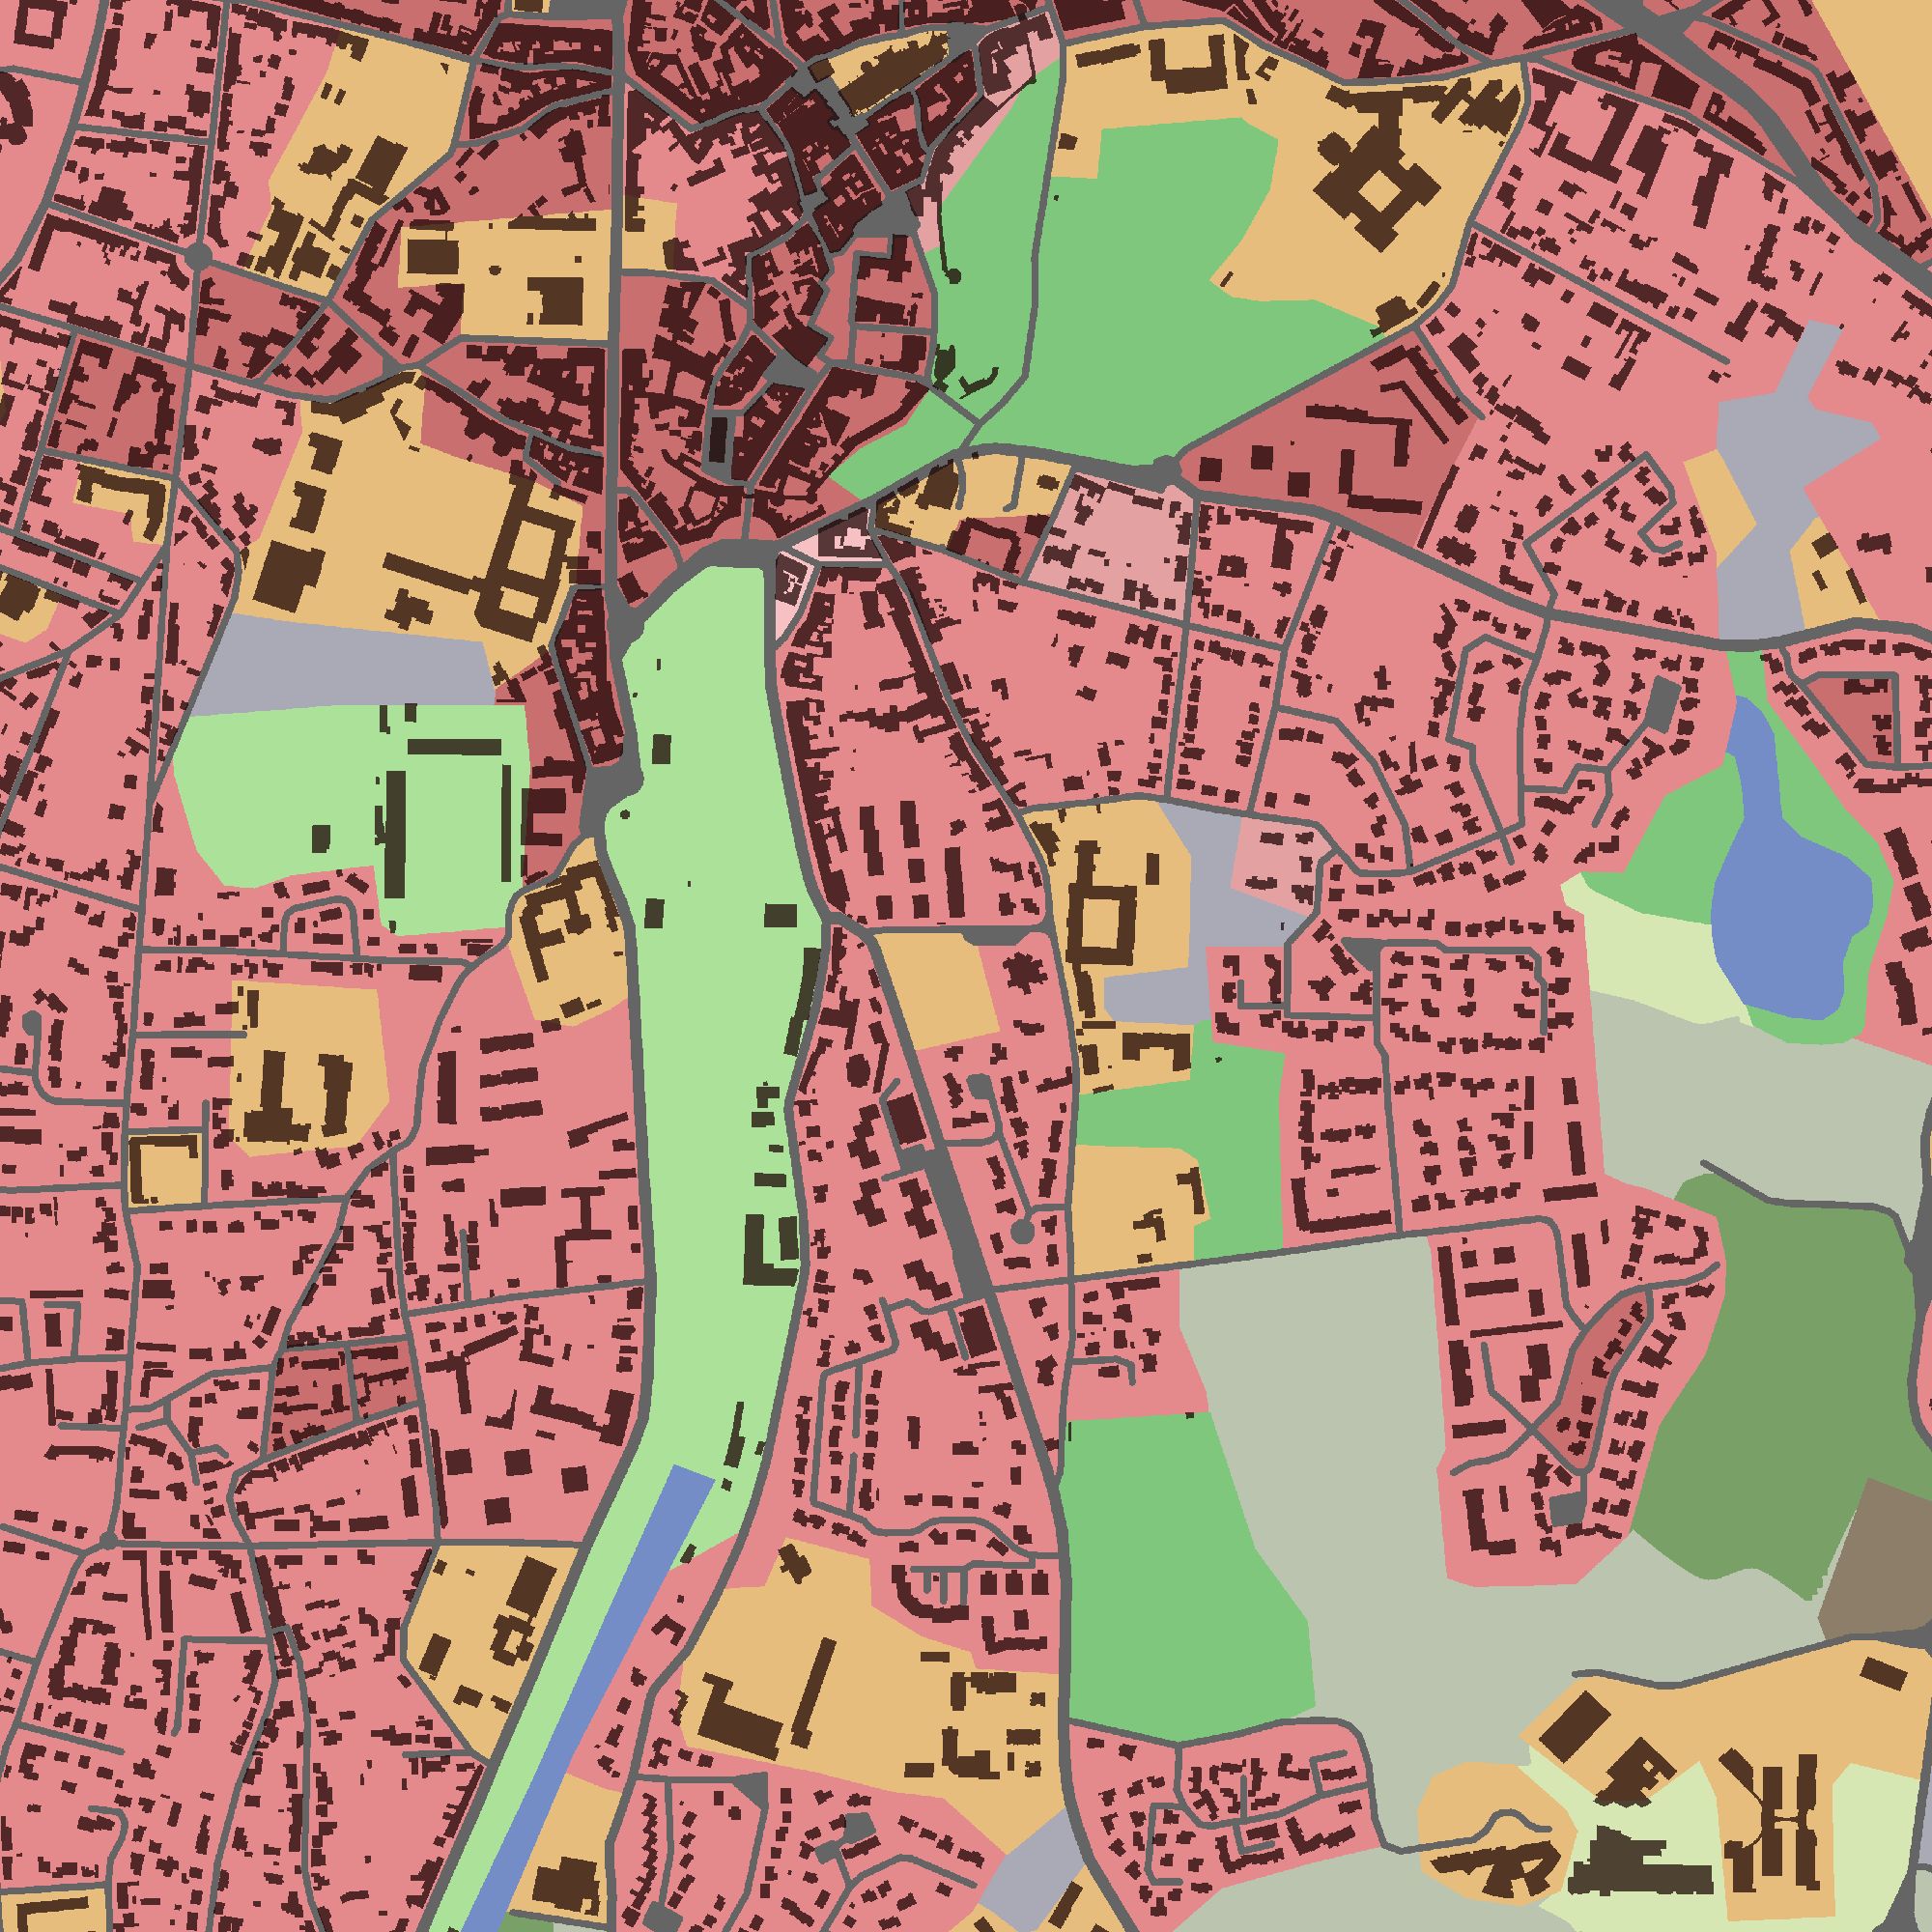
\includegraphics[width=4cm]{ua2012_buildings.png}};

\node[colblue,draw,line width=0.5mm,minimum width=0.2cm,minimum height=1cm] (portinua) at ($(ua.west)+(1.5,0.5)$) {};
\node[colred,draw,line width=0.5mm,minimum width=1cm,minimum height=0.7cm] (ubsinua) at ($(ua.south)+(1.5,0.35)$) {};
\node[colgreen,draw,line width=0.5mm,minimum width=0.7cm,minimum height=0.5cm] (jardinsinua) at ($(ua.north)+(0.25,-0.7)$) {};

\draw (interpout) edge[out=0,in=180,->,thick,colblue] node[above,xshift=-0.8cm,colblue!50!black] {Port} (portinua);
\draw ($(interpout)-(0,1.8)$) edge[->,out=0,in=-90,looseness=0.7,thick,colred] node[colred!50!black,below,yshift=-0.2cm] {Université} (ubsinua.south);
\draw ($(interpout)+(0,1.8)$) edge[->,in=90,out=0,thick,colgreen] node[colgreen!50!black,above,yshift=0.15cm] {Jardins} (jardinsinua.north);

\end{tikzpicture}

\end{document}
}
	\caption{Cartographie automatisée d'images aériennes.}
	\label{fig:semantic_mapping}
\end{figure}

Ce chapitre s'intéresse à la cartographie d'images aériennes à trois canaux, \glsfirst{RVB} ou \glsfirst{IRRV}, en \gls{THR} ($<50cm$) ou \gls{EHR} ($<10cm$). L'objectif étant d'étudier la possibilité d'appliquer des méthodes d'apprentissage profond utilisées en vision par ordinateur classique aux images de télédétection, nous nous intéressons dans un premier temps à des images présentant des caractéristiques proches des images multimédia\,: résolution élevée et espace de couleur \gls{RVB} ou assimilé, acquises par des appareils photo du commerce.

Nous souhaitons apprendre un modèle de cartographie sémantique à partir des images, c'est-à-dire capable d'associer une classe d'intérêt à chaque élément de l'image considérée (\cref{fig:semantic_mapping}). Formellement, il s'agit pour une image $I$ de dimensions $M \times N$ et d'un ensemble de classes d'intérêts numérotées de $1$ à $n$ d'associer à chaque pixel $I_{i,j}$ une classe $k_{i,j} \in \{1..n\}$. Nous allons donc chercher à approcher la fonction $f$ telle que\,:
\begin{equation}
	\forall (i,j) \in \{1\dots{}M\}\times\{1\dots{}N\}~~~f(I[i,j]) = k_{i,j}~.
\end{equation}

Contrairement au problème de la reconnaissance d'objet, qui associe une ou plusieurs étiquettes à une image dans son intégralité, il s'agit ici d'un problème de classification \emph{dense}. Compte-tenu du fait que l'on travaille sur des images et que les pixels $I[i,j]$ sont liés spatialement entre eux, on parle habituellement de segmentation sémantique. En effet, l'image ainsi classifiée pourra se représenter sous la forme d'une carte à partir de laquelle il est possible de regrouper les pixels voisins et sémantiquement liés pour former un ensemble de régions cohérentes.

Nous allons apprendre un modèle statistique permettant d'approcher $f$ en procédant en deux étapes. La première, dite d'extraction de caractéristiques, consiste à projeter l'information brute dans espace de représentation abstrait. La seconde consiste à séparer l'espace ainsi formé en sous-ensemble disjoints, c'est-à-dire à réaliser la classification à proprement parler.


Par exemple, dans le cas d'une \glssymbol{SVM} linéaire, la classification s'effectue en déterminant les hyperplans permettant de séparer au mieux les données. L'espace de représentation idéal est donc linéairement séparable. Il s'agit alors de trouver un extracteur de caractéristiques, c'est-à-dire une projection, transformant la donnée initiale en une représentation adéquate. Nous commençons par formaliser le problème puis nous rappellerons l'état de l'art en segmentation non supervisée, avant d'étudier les propriétés désirables de ces algorithmes dans le cadre de la classification par région d'images de télédétection.

\subsection{Classification par région}

Une première approche pour la segmentation sémantique consiste à mettre en \oe{}uvre sur l'image des classifieurs. Comme nous l'avons vu dans le chapitre précédent, la classification d'images est un domaine ayant largement été exploré dans la littérature. Ici, il s'agit non pas d'associer une image à une classe, mais de faire correspondre chacun des pixels de l'image à une classe. Toutefois, il est possible d'associer les deux problèmes en considérant séparément la segmentation et la sémantisation de l'image. L'image est découpée en plusieurs morceaux qui seront classifiés séparément. Il s'agit donc d'une classification par région. Dans un premier temps, un algorithme de segmentation permettra de partitionner l'image, puis le classifieur assignera à chacun des segment une des classes d'intérêt du problème.
\begin{definition}
La classification par région d'une image $I$ consiste à trouver une partition $P = {P_1, \dots, P_n}$ telle que\,:
$$\wbigcup_{i=1}^n P_i = I~~~\text{(segmentation)}$$
et une fonction $f$ telle que\,:
$$f(P_i) = k_i~~~\text{(classification)}$$
avec $k_i$ la classe d'intérêt associée à la $i$\ieme région\footnote{Par vote majoritaire, par exemple.}.
\end{definition}

Diverses approches ont été proposées dans la littérature en télédétection, utilisant par exemple des profils d'attributs sur des segmentations hiérarchiques arborescentes~\cite{bosilj_indexation_2016}, des segmentations de type superpixels combinées à une approche sac de mots visuels~\cite{li_superpixel-based_2018} ou encore des réseaux de neurones profonds~\cite{gong_superpixel-based_2017}. Dans un premier temps, nous passons en revue les méthodes de segmentation non-supervisée et nous étudions l'influence de celles-ci sur les performances des classifieurs utilisés dans le cadre de la classification par région.

\subsection{Algorithmes de segmentation}
\label{sec:segmentations}

Il existe de nombreux algorithmes de segmentation d'image non-supervisés. Les approches les plus anciennes traitent des images monochromes en niveaux de gris tandis que les plus récentes peuvent travailler dans espaces couleurs comme \gls{RVB}, teinte-saturation-intensité ou encore l'espace \gls{LAB}.

Une première famille de segmentation traite l'image sous la forme d'un graphe. Formellement, les pixels sont représentés par les n\oe{}uds du graphe dont les arêtes représentent les relations de similarité entre pixels voisins. La construction des régions de l'image se fait alors en agglomérant les nœuds du graphe en fonction des arêtes qui les relient. C'est sur ce principe que fonctionne l'algorithme de segmentation \gls{FH}~\cite{felzenszwalb_efficient_2004}, qui segmente l'image en calculant un arbre couvrant de poids minimal, mais aussi l'algorithme \emph{Normalized Cuts}~\cite{shi_normalized_2000} qui aborde le problème sous l'angle du partitionnement de graphe. C'est également l'approche utilisée pour les algorithmes à base de marche aléatoire sur le graphe de l'image, soit pour la minimisation d'une fonction entropie pour l'algorithme \gls{ERS}~\cite{liu_entropy_2011}, soit pour la résolution d'équation de diffusion~\cite{grady_random_2006}.

Une seconde approche, particulièrement populaire dans la littérature récente, utilise des algorithmes itératifs de \emph{clustering} (partitionnement de données) pour la segmentation. Ce procédé a engendré deux grandes familles de segmentations dites \og superpixels \fg. La première est dérivée de l'algorithme \gls{SLIC}~\cite{achanta_slic_2010}. Cet algorithme projette les pixels dans un espace de représentation couleur-$(x,y)$ de dimension 5 et utilise un algorithme de partitionnement itératif dérivé des $k$-moyennes. \gls{SLIC} initialise un nombre de centres déterminé par l'utilisateur sur une grille régulière, puis met à jour itérativement ceux-ci en absorbant les pixels voisins de la frontière des régions segmentées. Cette méthode vu naître plusieurs variantes, dont le \emph{Preemptive SLIC}~\cite{neubert_compact_2014}, plus rapide, l'algorithme \gls{LSC}~\cite{li_superpixel_2015} intégrant des contraintes globales en plus de la mise à jour itérative locale et l'algorithme \gls{SCALP}~\cite{giraud_robust_2018}. \gls{SCALP} interdit l'apparition de superpixels de forme non-régulière dans l'image en considérant l'ensemble des pixels sur le chemin entre le barycentre du superpixel et celui à ajouter. En outre, \gls{SCALP} prend en entrée le résultat d'un algorithme de détection de contours afin de renforcer l'adhérence des superpixels aux bordures des objets.
La deuxième grande famille d'algorithmes de segmentation superpixels se base sur le principe des $k$-médoïdes. En particulier, il s'agit de projeter les pixels dans un espace non-euclidien de dimension 5 (généralement \glssymbol{RVB}-$(x,y)$) puis de réaliser le partitionnement en cherchant le mode dominant local de chaque voisinage, c'est-à-dire la médoïde. Cette approche a notamment utilisée pour les algorithmes \emph{Mean Shift}~\cite{comaniciu_mean_2002} et \emph{Quickshift}~\cite{vedaldi_quick_2008}.
Plusieurs autres algorithmes utilisent également des approches itératives de partitionnement. L'algorithme \gls{SEEDS}~\cite{bergh_seeds_2012} définit ainsi des blocs de pixels capables d'échanger des éléments le long de leur frontière afin de maximiser une fonction d'énergie dépendant des histogrammes de couleurs. \gls{SEEDS} utilise une optimisation par \emph{hill-climbing} afin de faire converger itérativement les blocs vers une segmentation stable. Enfin, il existe également des algorithmes itératifs convergeant vers une segmentation à partir de la méthode des surfaces de niveau, comme l'algorithme de Chan-Vese~\cite{chan_active_1999} dérivé des contours actifs ou l'algorithme \emph{TurboPixel}~\cite{levinshtein_turbopixels_2009} considérant localement la courbure et le gradient de l'image.

Pour la segmentation d'images en niveaux de gris, l'approche morphologique \emph{watershed} (ou segmentation par ligne de partage des eaux)~\cite{beucher_morphological_1993} est particulièrement populaire. \emph{Watershed} considère l'image comme une carte d'élévation dans laquelle est simulée l'élévation du niveau de l'eau. Initialement, l'eau s'écoule depuis un certain de nombre de sources positionnées sur des marqueurs, qui peuvent être insérés manuellement ou calculés automatiquement, par exemple aux extrema locaux du gradient de l'image. L'eau remplit alors le relief topographique et le niveau est artificiellement augmenté. Lorsque deux sources se rencontrent, un barrage virtuel est érigé à leur ligne de démarcation, établissant ainsi une des frontières de la segmentation. L'algorithme s'arrête lorsque toute l'image a été inondée. Le choix des marqueurs initiaux de \emph{watershed} est critique pour la qualité de la segmentation et notamment à la régularité des régions produites. Une version dite compacte a été proposée~\cite{neubert_compact_2014} afin de rendre \emph{watershed} robuste à l'initialisation, en la rendant plus proche de~\gls{SLIC}. L'approche morphologique peut également être utilisée dans le cadre des contours actifs, notamment dans une variante de l'algorithme Chan-Vese~\cite{chan_active_1999} utilisant les contours actifs morphologiques~\cite{marquez-neila_morphological_2014}.

Enfin, des algorithmes spécifiques au traitement d'images télédétection, notamment radar et multispectrales, ont été proposées dans la littérature. Ces segmentation prennent notamment en compte des aspects multi-échelles avec pour objectif final l'analyse d'image orientée objet. Ainsi, l'algorithme \gls{MRS}~\cite{baatz_multiresolution_2000} est une méthode populaire de segmentation d'images de télédétection, notamment grâce à son implémentation dans le logiciel eCognition\copyright. \gls{MRS} se focalise sur l'identification d'objets saillants dans l'image sur lesquels définir une segmentation. \gls{MRS} utilise une approche par croissance de régions selon un critère d'homogénéité spectrale défini de façon heuristique. \gls{MRS} exécute une segmentation à plusieurs échelles et choisit de conserver ou de fusionner les régions les plus fines selon un critère de similarité.
L'algorithme \gls{HSEG}~\cite{tilton_best_2012} quant à lui produit un segmentation hiérarchique multi-échelles. En effet, \gls{HSEG} produit plusieurs segmentations, organisées sous forme d'arbre\,: une région de l'échelle la plus grande est sous-divisée en plusieurs régions, elles-mêmes pouvant être divisée récursivement. \gls{HSEG} utilise une approche par croissance de régions dans laquelle les pixels proches sont itérativement fusionnés à moins de vérifier un critère spécifique de dissimilarité. Des régions voisines peuvent ensuite être elles-même fusionnées en cas d'homogénéité, afin de produire une segmentation hiérarchique à une échelle plus faible.

\begin{figure}[t]
\foreach \picname\path in {Image originale/fox,SLIC/fox_slic,Quickshift/fox_quickshift,Algorithme MRS/fox_ecognition,FH/fox_felzenszwalb,Watershed/fox_watershed}
{
\begin{subfigure}{0.33\textwidth}
    \includegraphics[width=\textwidth]{\path}
    \includegraphics[width=\textwidth]{\path_patchwork}
    \caption*{\picname}
\end{subfigure}%
}
\caption{Segmentations d'une image naturelle. Certains algorithmes produisent des régions faiblement régulières, mais capturant mieux les détails de l'image. {\small Crédits image originale\,: \href{https://pixabay.com/en/mammals-wildlife-expensive-fox-3218028/}{Tom Frydenlund, CC0}.}}
\label{fig:fox_segmentation}
\end{figure}

\begin{figure}[t]
\foreach \picname\path in {Image originale/potsdam,SLIC/potsdam_slic,Quickshift/potsdam_quickshift,Algorithme MRS/potsdam_ecognition,FH/potsdam_felzenszwalb,Watershed/potsdam_watershed}
{
\begin{subfigure}{0.33\textwidth}
    \includegraphics[width=\textwidth]{\path}
    \includegraphics[width=\textwidth]{\path_patchwork}
    \caption*{\picname}
\end{subfigure}%
}
\caption{Segmentations d'une image aérienne du jeu de données \gls{ISPRS} Potsdam. Selon l'algorithme appliqué, les voitures sont plus ou moins bien segmentées.}
\label{fig:potsdam_segmentation}
\end{figure}


\subsection{Choix de la méthode de segmentation}

Face à la profusion de méthodes de segmentation existantes vient la question du choix de celle le plus adapté pour l'apprentissage statistique de modèles de classification. Deux critères sont à prendre en compte\,: quels pré-traitements est-il nécessaire d'appliquer à l'image, et quelle segmentation semble respecter au mieux les propriétés spatiales de l'image?


\subsubsection{Pré-traitement de l'image}
La plupart des algorithmes de segmentation recommandent de traiter au préalable l'image à segmenter en lui appliquant un flou gaussien plus ou moins prononcé. Ce prétraitement se justifie en cela qu'il adoucit les bordures et réduit l'influence du bruit dans l'image, facilitant la segmentation. Empiriquement, pour des images aériennes, un léger flou gaussien suffit à obtenir des segmentations superpixels cohérentes. L'application de ce flou ne sert qu'à la segmentation, et peut bien entendu être abandonnée au moment de la classification.

La segmentation se fait dans la plupart des cas dans l'espace de couleurs \gls{LAB}. Cet espace de couleurs est conçu pour refléter la vision humaine, en particulier la courbe de réponse de l'\oe{}il humain aux variations de couleurs, qui est logarithmique plutôt que linéaire. Cependant, cela nécessite de s'interroger sur la pertinence d'une telle conversion lorsque les trois canaux des images aériennes ne sont pas \gls{RVB}, mais \gls{IRRV} par exemple. En pratique, cela ne semble pas poser de problèmes, mais ces techniques de segmentation ne se généraliseront donc pas nécessairement telles quelles pour des images dont la structure est différente du \gls{RVB} traditionnel, en particulier pour le traitement d'images multispectrales. Seuls les algorithmes \gls{MRS} et \gls{HSEG} ont été conçus avec la télédétection comme application finale.

\subsubsection{Forme et tailles des régions}

Plusieurs analyses préliminaires~\cite{neubert_superpixel_2012,achanta_slic_2012,stutz_superpixels_2018} montrent que les différents algorithmes de segmentation peuvent avoir des propriétés très différentes. Notamment, différents algorithmes ne sont pas robustes aux mêmes perturbations et ne segmentent pas les images de la même façon. Notamment, la plupart des algorithmes de segmentation par partitionnement de graphes tendent à ne pas donner à l'utilisateur de contrôle sur la forme et la compacité des régions segmentées. Un exemple qualitatif de segmentation sur une image naturelle est donné dans la~\cref{fig:fox_segmentation}.

Le premier constat qu'il est possible d'en tirer est que les différentes familles d'algorithmes génèrent des segmentations d'aspect variable. L'algorithme de segmentation \gls{FH} génère par exemple des régions de taille et de forme très hétérogènes. En effet, \gls{FH} n'est pas contraint dans son exploration de l'image, et parvient ainsi à rassembler de très grandes surfaces (notamment des routes) dans une unique région. Ce partitionnement peut ainsi conduire à des régions de quelques pixels quand d'autres recouvrent une large portion de l'image, sans qu'aucun paramètre ne puisse contrôler cette variabilité.

À l'opposé, les méthodes de type superpixels et plus particulièrement les dérivés de \gls{SLIC}, donnent des résultats visuellement réguliers. Cette propriété s'accroît lorsque le paramètre de compacité est augmenté afin de contraindre l'adhérence à la grille. Notamment, il est assez aisé de maintenir les superpixels segmentés par \gls{SLIC} à une taille raisonnable tout en leur laissant une certaine liberté de forme. Quickshift se comporte de manière similaire, bien que les superpixels générées soient nettement plus irréguliers que dans les méthodes dérivées de~\gls{SLIC}, ce qui produit des artefacts dans la segmentation. La segmentation \emph{watershed} compacte présente des caractéristiques très similaires aux méthodes de superpixels, et il est préférable de l'utiliser tant l'approche classique est sensible au choix des marqueurs. Ces analyses sont conformes aux études de la littérature~\cite{neubert_superpixel_2012,achanta_slic_2012}. Dans l'ensemble, de nombreuses variantes d'algorithme de superpixels ont été développées et présentes des caractéristiques similaires~\cite{stutz_superpixels_2018}.

Toutefois, l'application finale étant la classification d'images de télédétection, il est intéressant d'étudier le comportement des algorithmes de segmentation sur des données prises à la verticale du sol. Un exemple est illustré dans la~\cref{fig:potsdam_segmentation}. L'algorithme \gls{MRS} semble particulièrement adapté aux images de télédétection. En effet, bien que la segmentation paraisse visuellement chaotique, la composition de l'image est respectée jusque dans les moindres détails. Les algorithmes de type superpixels tendent à faire disparaître les détails, et notamment les véhicules, ce qui peut poser problème pour les approches de modélisation d'objets.

Compte-tenu de cette analyse, nous étudierons en priorité les algorithmes de segmentation prévus pour la télédétection (\gls{HSEG} et \gls{MRS}) ainsi qu'un représentant des deux grandes familles de segmentation compacte\,: Quickshift et \gls{SLIC}. Les approches \emph{watershed} sont écartées compte-tenu de leur forte proximité avec \gls{SLIC}~\cite{neubert_compact_2014} tandis que l'approche \gls{FH} est éliminée de part sa grande variabilité entre régions~\cite{neubert_superpixel_2012}.

\section{Réseaux de neurones profonds}

\subsection{Réseaux de neurones convolutifs comme extracteurs de caractéristiques}

L'intérêt majeur de l'apprentissage profond réside dans l'apprentissage des représentations~\cite{bengio_representation_2013,goodfellow_deep_2016}. En effet, à partir des images d'entrées, nous avons vu que les réseaux convolutifs réalisent une extraction de caractéristique. Cette projection dans un espace de représentation est réalisée par les premières couches, qui sont elles-mêmes optimisables. Autrement dit, la représentation apprise est optimisée pour la tâche de classification sur les données d'entraînement.

Il est donc possible de fournir une image à un \gls{CNN} et d'arrêter le calcul des activations avant la dernière couche. Les activations ainsi obtenues peuvent se représenter sous la forme d'un vecteur de caractéristiques.

Les caractéristiques ainsi extraites peuvent ensuite être utilisées pour entraîner un classifieur de façon habituelle. Cette approche est similaire au principe de spécialisation d'un réseau par \emph{fine-tuning}. En particulier, il a été montré dans~\cite{razavian_cnn_2014} que l'utilisation des caractéristiques extraites par un réseau pré-entraîné sur le jeu de données ImageNet~\cite{deng_imagenet_2009} pour entraîner une \gls{SVM} linéaire donnait d'excellents résultats sur la plupart des tâches visuelles.~\cite{razavian_cnn_2014} défend ainsi l'idée qu'il s'agit d'une méthode simple à mettre en \oe{}uvre et qui permet d'obtenir immédiatement des résultats satisfaisants, généralement meilleurs que ceux obtenues avec les caractéristiques classiques (\gls{HOG}, \gls{SIFT}\dots). Il est intéressant de constater que les représentations apprises par les réseaux convolutifs sont généralement de meilleurs points de départ pour l'optimisation que des initialisations aléatoires, même dans le cas de tâches très différentes~\cite{yosinski_how_2014}.

Ces résultats ont été repris et confirmés dans~\cite{penatti_deep_2015,marmanis_deep_2016,lagrange_benchmarking_2015} pour la classification d'images aériennes, établissant des nouveaux états de l'art sur des jeux de données comme UC Merced et \emph{Brazilian Coffe}. En particulier,~\cite{marmanis_deep_2016,penatti_deep_2015} ont montré  qu'il est possible d'utiliser les caractéristiques extraites par un réseau pré-entraîné sur ImageNet pour la classification d'images aériennes et satellitaires, ce qui a été étendu à la segmentation sémantique par région par la suite~\cite{lagrange_benchmarking_2015}. Ce résultat est contre-intuitif dans la mesure où les images de la base ImageNet sont des images multimédia classiques\,: animaux, objets du quotidien, personnes, paysages\dots La généricité des filtres les rend néanmoins adaptables à de nombreux contextes, y compris la télédétection.

\subsubsection{Application à la cartographie sémantique}

\begin{figure}
\resizebox{\textwidth}{!}{%
\documentclass{standalone}
\usepackage[utf8]{inputenc}
\usepackage[T1]{fontenc}
\usepackage{tikz}
%%%%%%%%%%%%%%%%%%%%%%%%%%%%%%%%%%%%%%%%
%           Commandes perso            %
%%%%%%%%%%%%%%%%%%%%%%%%%%%%%%%%%%%%%%%%

%% Figures centrées, et en position 'here, top, bottom or page'
\newenvironment{figureth}{%
		\begin{figure}[htbp]
			\centering
	}{
		\end{figure}
		}


%% Tableaux centrés, et en position 'here, top, bottom or page'
\newenvironment{tableth}{%
		\begin{table}[htbp]
			\centering
			%\rowcolors{1}{coleurtableau}{coleurtableau}
	}{
		\end{table}
		}

%% Sous-figures centrées, en position 'top'
\newenvironment{subfigureth}[1]{%
	\begin{subfigure}[t]{#1}
	\centering
}{
	\end{subfigure}
}

\newcommand{\citationChap}[2]{%
	\epigraph{\og \textit{#1} \fg{}}{#2}
}

%% On commence par une page impaire quand on change le style de numérotation de pages
\let\oldpagenumbering\pagenumbering
\renewcommand{\pagenumbering}[1]{%
	\cleardoublepage
	\oldpagenumbering{#1}
}

%% Légende du dataset ISPRS
\newcommand\isprslegende{
Légende\,: \textcolor{Black}{blanc}\,: routes, \textcolor{Blue}{bleu}\,: bâtiments, \textcolor{Cerulean}{cyan}\,: végétation basse, \textcolor{OliveGreen}{vert}\,: arbres, \textcolor{Dandelion}{jaune}\,: véhicules, \textcolor{BrickRed}{rouge}\,: autre.
}

%% Dessiner des réseaux de neurones avec Tikz
\newcommand{\convlayer}[9]{%{h}{w}{d}{name}{color}{x}{y}{z}%{note w}{note h}{note d}
   \def\h{#1}
   \def\w{#2}
   \def\d{#3}
   \def\name{#4}
   \ifthenelse {\equal{#5} {}} {\def\col{white}} {\def\col{#5}}
   \def\x{#6}
   \ifthenelse {\equal{#7} {}} {\def\y{0}} {\def\y{#7}}
   \ifthenelse {\equal{#8} {}} {\def\z{0}} {\def\z{#8}}
   % ne faites pas ça chez vous !
   \ifthenelse {\equal{#9} {}} {\convlayercontinued{}{}{}} {\convlayercontinued#9}
}

\newcommand\convlayercontinued[3]{
   \def\notew{#1}
   \def\noteh{#2}
   \def\noted{#3}
   \coordinate (A) at (\x-\d/2,  \y-\h/2, \z-\w/2);
   \coordinate (B) at (\x-\d/2,  \y-\h/2, \z+\w/2);
   \coordinate (C) at (\x-\d/2,  \y+\h/2, \z+\w/2);
   \coordinate (D) at (\x-\d/2,  \y+\h/2, \z-\w/2);
   \coordinate (E) at (\x+\d/2,  \y-\h/2, \z-\w/2);
   \coordinate (F) at (\x+\d/2,  \y-\h/2, \z+\w/2);
   \coordinate (G) at (\x+\d/2,  \y+\h/2, \z+\w/2);
   \coordinate (H) at (\x+\d/2,  \y+\h/2, \z-\w/2);

    \draw [draw opacity=0.3, fill opacity=0.8, fill=\col!60!white] (A) -- (B) -- (C) -- (D) -- cycle;
    \draw [draw opacity=0.3, fill opacity=0.8, fill=\col!60!white] (A) -- (B) -- (F) -- (E) -- cycle;
    % Face haut
    %\draw [left color=\col!60!white, right color=\col!80!white, shading=axis, shading angle=180] (C) -- (D)  -- (H) -- (G) -- cycle;
    \draw [fill opacity=0.9, fill=\col!70!white] (C) -- node[rotate=45,above] {\small \name} (D) -- (H) -- (G) -- cycle;
    %\draw [fill opacity=0.9, fill=\col!70!white] (C) -- (D) -- node[above] {\small \name} (H) -- (G) -- cycle;
    % Face droite
    \draw [fill opacity=0.9, fill=\col!60!white] (E) -- node[pos=0.75,rotate=45,below] {\scriptsize \notew} (F) -- (G) --  (H) -- cycle;
    % Face avant
    %\draw [shading=axis, left color=\col!60!white, right color=\col!40!white, shading angle=-45] (B) -- node[above,rotate=90] {\scriptsize \noteh} (C) -- (G) -- (F) -- node[below] {\scriptsize \noted}  cycle;
    \draw [fill opacity=0.9, fill=\col!50!white] (B) -- node[above,rotate=90] {\scriptsize \noteh} (C) -- (G) -- (F) -- node[below] {\scriptsize \noted}  cycle;
}

\newcommand{\fclayer}[8]{%{h}{w}{name}{color}{x}{y}{z}
   \def\h{#1}
   \def\w{#2}
   \def\name{#3}
   \ifthenelse {\equal{#4} {}} {\def\col{white}} {\def\col{#4}}
   \def\x{#5}
   \def\y{#6}
   \def\z{#7}
   \def\note{#8}
   \coordinate (A) at (\x-\w/2,  \y-\h/2, \z);
   \coordinate (B) at (\x+\w/2,  \y-\h/2, \z);
   \coordinate (C) at (\x+\w/2,  \y+\h/2, \z);
   \coordinate (D) at (\x-\w/2,  \y+\h/2, \z);

   \pgfmathparse{4*\w}\let\boxwidth\pgfmathresult
    \draw [fill=\col] (A) -- node[below,text width=\boxwidth cm,align=center] {\scriptsize \note} (B) -- (C) -- (D) -- cycle;

    \node (N) at ($(A)!0.5!(B)+(0,-1,0)$) {\name};
}

\newcommand{\alexnet}[4]{%{scale}{x}{y}{z}
  \def\scale{#1}
  \def\alexx{#2}
  \def\alexy{#3}
  \def\alexz{#4}


  \def\coblue{blue!50!white}
  \def\fcgrey{gray!50!white}

  \convlayer{1.3*\scale}{1.3*\scale}{0.02*\scale}{Image}{\coblue}{\alexx}{\alexy}{\alexz}{{227}{227}{3}}
  \convlayer{1.1*\scale}{1.1*\scale}{0.08*\scale}{Conv1}{\coblue}{\alexx+0.7*\scale}{\alexy}{\alexz}{{55}{55}{96}}
  \convlayer{0.7*\scale}{0.7*\scale}{0.5*\scale}{Conv2}{\coblue}{\alexx+1.5*\scale}{\alexy}{\alexz}{{27}{27}{256}}
  \convlayer{0.5*\scale}{0.5*\scale}{0.8*\scale}{Conv3}{\coblue}{\alexx+2.6*\scale}{\alexy}{\alexz}{{13}{13}{384}}
  \convlayer{0.5*\scale}{0.5*\scale}{0.8*\scale}{Conv4}{\coblue}{\alexx+3.8*\scale}{\alexy}{\alexz}{{13}{13}{384}}
  \convlayer{0.5*\scale}{0.5*\scale}{0.5*\scale}{Conv5}{\coblue}{\alexx+4.8*\scale}{\alexy}{\alexz}{{13}{13}{256}}
  \fclayer{\scale}{0.1*\scale}{FC1}{\fcgrey}{\alexx+5.4*\scale}{\alexy}{\alexz}{4096}
  \fclayer{\scale}{0.1*\scale}{FC2}{\fcgrey}{\alexx+5.7*\scale}{\alexy}{\alexz}{4096}
  \fclayer{\scale}{0.1*\scale}{FC3}{\fcgrey}{\alexx+6.0*\scale}{\alexy}{\alexz}{1000}
}

\newcommand{\imagelayer}[7]{%{width}{x}{y}{z}{path}{text_up}{text_down}
    \pgfmathparse{#1}\let\w\pgfmathresult
    \begin{scope}[canvas is yz plane at x=#2]
     \node[transform shape] (source) at (#3, #4) {\includegraphics[angle=-90,width=\w cm]{#5}};
    \end{scope}
     \node [transform shape, rotate=45, above] at (source.east) {#6};
     \node [transform shape, rotate=45, below] at (source.west) {\scriptsize{#7}};
}

\def\fourier{\mathcal{F}}

\newcommand{\lightspectrum}{%
\pgfplotsset{
    % this *defines* a custom colormap ...
    colormap={slategraywhite}{color(0cm)=(red); color(1cm)=(red); color(2cm)=(red); color(3cm)=(red); color(4cm)=(orange); color(5cm)=(yellow); color(6cm)=(green); color(7cm)=(blue); color(8cm)=(blue); color(9cm)=(purple); color(10cm)=(purple); color(12cm)=(black)}
}
\node at (1.5, 2.7) {\small 1mm};
\node at (4, 3) {Infrarouge};
\node at (7.75, 2.7) {\small 800nm};
\node at (9, 3) {Visible};
\node at (10.5, 2.7) {\small 400nm};
\node at (12, 3) {Ultraviolet};
\node at (13.5, 2.7) {\small 10nm};
\draw[->] (1, 2.5) -- (14, 2.5);
\begin{axis}[hide axis,width=16cm,height=4cm,colormap name=slategraywhite]
\addplot[domain=20:1000,samples=1500,ultra thick, point meta=x*x,mesh]{sin(x*x/80)};
\end{axis}
}

% Union généralisée
\newcommand{\wbigcup}{\mathop{\bigcup}\displaylimits}

\newcommand{\res}[2]{#1 {\footnotesize $\pm$ #2}}
\newcommand{\bres}[2]{\textbf{#1} {\footnotesize $\pm$ #2}}
\newcommand{\bbres}[2]{\res{\textit{#1}}{#2}}

\newcommand{\drawkernel}[9]{
\begin{tikzpicture}
	\draw[step=1cm,gray!50!white,very thin] (0,0) grid (3,3);
	\kernelnode{0.5}{0.5}{#1};
	\kernelnode{0.5}{1.5}{#2};
	\kernelnode{0.5}{2.5}{#3};
	\kernelnode{1.5}{0.5}{#4};
	\kernelnode{1.5}{1.5}{#5};
	\kernelnode{1.5}{2.5}{#6};
	\kernelnode{2.5}{0.5}{#7};
	\kernelnode{2.5}{1.5}{#8};
	\kernelnode{2.5}{2.5}{#9};
\end{tikzpicture}
}

\newcommand{\kernelnode}[3]{%{x}{y}{value}
	\ifthenelse{\equal{#3}{0}}{
		\def\kcolor{gray}
	}{
		\def\kcolor{black}
	}
	\node[\kcolor] at (#1, #2) {#3};
}

\newcommand{\chapsummary}[1]{
\section*{Résumé du chapitre :}
\parbox{0.9\linewidth}{
\setlength{\parindent}{4ex}
#1}
}

\newcommand{\eqname}[1]{\tag*{\small (#1)}}

\begin{document}

\begin{tikzpicture}[]
\usetikzlibrary{3d}
\usetikzlibrary{calc}
\usetikzlibrary{arrows.meta, bending}

\coordinate (input) at (0, 2);
\coordinate (seg) at (0,-3);
\coordinate (patches) at (5, 0);
\coordinate (net) at (11.5, 0);
\coordinate (features) at (16.5, 0);
\coordinate (classifier) at (19, 0);
\coordinate (map) at (24, 0);

\node (in_fig) at (input) {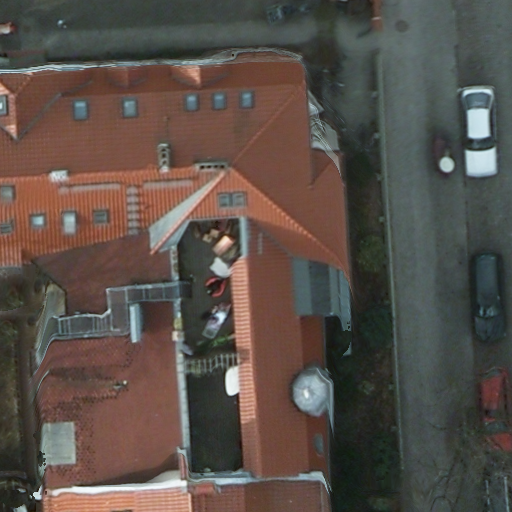
\includegraphics[width=3cm]{orthohr_rgb}};
\node[yshift=4pt] at (in_fig.north) {Image initiale};

\node (seg_fig) at (seg) {\includegraphics[width=3cm]{orthohr_rgb_slic}};
\node[yshift=-4pt] at (seg_fig.south) {Image segmentée};

\draw[ultra thick,->] ([xshift=0.8cm]in_fig.south) to node[left]{\small segmentation} ([xshift=0.8cm]seg_fig.north);

\node (large) at ($ (patches)+(0,2.5)$) {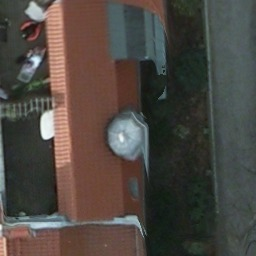
\includegraphics[width=2cm]{large}};
\node[yshift=-3pt] at (large.south) {contexte};
\node (medium) at (patches) {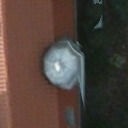
\includegraphics[width=2cm] {medium}};
\node[yshift=-3pt] at (medium.south) {contexte};
\node (ndsm) at ($ (patches)-(0,2.5) $) {\includegraphics[width=2cm]{ndsm}};
\node[yshift=-3pt] at (ndsm.south) {MNH};

\fill[line width=3pt,draw=red!95!black,fill=cyan!80!white,fill opacity=0.5,shading=axis, shading angle=135] (seg_fig.east) ++(-1.6,-1.1) --  +(0.6,0) -- +(0.6,0.6) -- +(0,0.6) -- cycle;

\draw (seg_fig.east) edge[in=180,out=0,->] (medium.west);
\draw (seg_fig.east) edge[in=180,out=0,->,looseness=0.8] (large.west);
\draw (seg_fig.east) edge[in=180,out=0,->] (ndsm.west);

\node[align=center] at ($ (patches)-(0,4.5) $) {Entrées multi-sources\\ et multi-échelles};

\node (net_fig) at (net) {\includegraphics[width=8cm]{../alexnet}};
\node at ($ (net) - (0,2)$) {CNN pré-entraîné};

\draw (large.east) edge[in=180,out=0,->] ([yshift=8pt]net_fig.west);
\draw (medium.east) edge[in=180,out=0,->] (net_fig.west);
\draw (ndsm.east) edge[in=180,out=0,->] ([yshift=-8pt]net_fig.west);

\coordinate (A) at ($ (features)+(0,-3,-0.5)$);
\coordinate (B) at ($ (features)+(0,3,-0.5)$);
\coordinate (C) at ($ (features)+(0.5,3,-0.5)$);
\coordinate (D) at ($ (features)+(0.5,-3,-0.5)$);
\coordinate (E) at ($ (features)+(0,-3,0)$);
\coordinate (F) at ($ (features)+(0,3,0)$);
\coordinate (G) at ($ (features)+(0.5,3,0)$);
\coordinate (H) at ($ (features)+(0.5,-3,0)$);

\coordinate (I) at ($ (E)!0.33!(F)$);
\coordinate (J) at ($ (E)!0.66!(F)$);
\coordinate (K) at ($ (H)!0.33!(G)$);
\coordinate (L) at ($ (H)!0.66!(G)$);
\coordinate (M) at ($ (D)!0.33!(C)$);
\coordinate (N) at ($ (D)!0.66!(C)$);

\def\grey{gray!40!white}
\draw[fill=\grey] (A) -- (B) -- (C) -- (D) -- cycle;
\draw[fill=\grey!60!white] (E) -- (F) -- (G) -- (H) -- cycle;
\draw[fill=\grey] (B) -- (C) -- (G) -- (F) -- cycle;
\draw[fill=\grey] (C) -- (D) -- (H) -- (G) -- cycle;
\draw[dotted,thick] (I) -- (K) -- (M);
\draw[dotted,thick] (J) -- (L) -- (N);
\node[align=center] at ($ (features) - (0,4.5)$) {Caractéristiques\\ profondes};

\draw ([yshift=-8pt]net_fig.east) edge[out=0,in=180,->] ($(I)!0.5!(E)$);
\draw ([yshift=8pt]net_fig.east) edge[out=0,in=180,->] ($(J)!0.5!(F)$);
\draw (net_fig.east) edge[out=0,in=180,->] ($(F)!0.5!(E)$);

\coordinate (c_A) at ($ (classifier) + (-1,1.5)$);
\coordinate (c_B) at ($ (classifier) + (-1,-1.5)$);
\coordinate (c_C) at ($ (classifier) + (1,-1.5)$);
\coordinate (c_D) at ($ (classifier) + (1,1.5)$);
\coordinate (c_top) at ($(c_A)!0.5!(c_D)$);
\coordinate (c_bottom) at ($ (c_B)!0.5!(c_C)$);
\filldraw[fill=yellow!50!white] (c_A) rectangle (c_C);


\newcommand\children[3]{
\coordinate (#1_c1) at ($(#1)!0.5!(#2)$);
\filldraw[fill=black] (#1_c1) circle (0.08);
\draw (#1) -- (#1_c1);
\coordinate (#1_c2) at ($(#1)!0.5!(#3)$);
\filldraw[fill=black] (#1_c2) circle (0.08);
\draw (#1) -- (#1_c2);
}

\coordinate (c_center) at ($(c_A)!0.5!(c_C)$);
\coordinate (c_center) at ($(c_center)!0.75!(c_top)$);
\filldraw[fill=black] (c_center) circle (0.1);
\coordinate (n1) at ($(c_center)!0.25!(c_B)$);
\filldraw[fill=black] (n1) circle (0.08);
\draw (c_center) -- (n1);
\coordinate (n2) at ($(c_center)!0.25!(c_C)$);
\filldraw[fill=black] (n2) circle (0.08);
\draw (c_center) -- (n2);

\children{n2}{c_bottom}{c_C}
\children{n2_c2}{c_bottom}{c_C}

\children{n1}{c_B}{c_bottom}
\children{n1_c1}{c_B}{c_bottom}

\node at ($(classifier) - (0,2)$) {Classifieur};

\draw ($(G)!0.5!(H)$) edge[ultra thick,in=180,out=0,->]  ($(c_A)!0.5!(c_B)$);

\node (map_fig) at (map) {\includegraphics[width=3cm]{gt_boundaries}};
\node[yshift=-4pt] at (map_fig.south) {Carte sémantique};
\fill[line width=3pt,draw=red!95!black,fill=cyan!50!white,fill opacity=0.2] (map_fig.east) ++(-1.6,-1.1) --  +(0.6,0) -- +(0.6,0.6) -- +(0,0.6) -- cycle;

\draw ($(c_C)!0.5!(c_D)$) edge[ultra thick,in=180,out=0,->] node[yshift=4pt,above]{Prédiction} node[yshift=-4pt,below]{\color{blue} ``Bâtiment''} (map_fig.west);

\end{tikzpicture}

\end{document}

}
\caption{Segmentation sémantique par régions d'une image aérienne. Chaque région de l'image segmentée est classifiée à partir de caractéristiques profondes extraites d'un réseau convolutif pré-entraîné.}
\label{fig:framework}
\end{figure}

À partir des procédés de segmentation et des méthodes de classification décrites précédemment, nous pouvons donc construire un processus complet de segmentation sémantique d'une image aérienne, repris de la~\cref{fig:framework}\,:
\begin{enumerate}
    \item Diviser l'image en sous-régions homogènes à l'aide d'un algorithme de segmentation.
    \item Pour chaque région, extraire une pyramide d'images de dimensions $32\times32$, $64\times64$ et $128\times128$ autour du centroïde de la région pour intégrer différents niveaux de contexte spatial.
    \item Extraire les caractéristiques de chaque imagette.
    \item Concaténer les vecteurs résultants dans un unique vecteur de caractéristique.
\end{enumerate}

Les échantillons d'apprentissage ainsi obtenus peuvent être utilisés pour entraîner le classifieur durant la phase d'apprentissage, ou simplement pour la prédiction en phase d'évaluation.

Dans le cas où l'extraction de caractéristiques est réalisée par un réseau convolutif, il est nécessaire de redimensionner l'imagette à la taille requise par le réseau (par exemple, $228\times228$ pour l'architecture AlexNet). Cette nécessité provient de la présence de couches entièrement connectées, qui contraignent la taille de la caractéristique obtenue en sortie de couches convolutives, et donc les dimensions initiales de l'image.

En outre, dans certains cas, la taille du vecteur de caractéristique est particulièrement grande. Pour AlexNet, la caractéristique obtenue est un vecteur de taille $1 000$ pour chaque imagette. Une région donnée génère donc un vecteur de taille $3 000$. L'optimisation exacte d'une \gls{SVM} en dimension 3 000 sur un grand jeu de données étant extrêmement long, nous utilisons l'approche de~\citet{bottou_large-scale_2010} utilisant une approximation des vecteurs des support par descente de gradient stochastique. Les résultats de cette approche seront détaillés dans la~\cref{sec:results_region}.

\subsection{Réseaux de neurones entièrement convolutifs}

Les méthodes de classification par région présentent deux inconvénients majeurs. Tout d'abord, le niveau de détail de la carte sémantique finale est fortement limité par l'algorithme de segmentation utilisé. En effet, si l'algorithme produit des régions grossières, alors la carte sémantique le sera également, car la classification ne permet d'associer qu'une seule étiquette à chacune des régions traitées. Pour augmenter la résolution, il est alors nécessaire de produire des régions plus petites mais donc plus nombreuses, augmentant ainsi proportionnellement le temps de calcul nécessaire au traitement de l'intégralité de l'image.

Une solution possible consiste à utiliser les réseaux de neurones entièrement convolutifs. Comme présenté dans le~\cref{chap:etat}, les \glsfirst{FCN} sont des réseaux comportant uniquement des couches de convolution et conçus pour réaliser une classification dense. Ainsi, chaque pixel de l'image initiale peut se retrouver associée à une classe d'intérêt en une seule inférence.

Cette solution présente plusieurs avantages\,:
\begin{itemize}
	\item La prédiction concernant une pixel prend automatiquement en compte le contexte spatial qui l'entoure,
	\item Les images d'entrée n'ont pas nécessairement une taille fixée \emph{a priori},
	\item La classification dense résultante est calée sur la grille des pixels, c'est-à-dire à la même résolution que l'image.
\end{itemize}

Les \gls{FCN} peuvent ainsi être utilisés pour traiter de grandes images en une passe unique, sans nécessiter de segmentation préalable. L'extraction de caractéristiques est automatiquement réalisée de façon dense et se fait conjointement à la classification. Les représentations apprises pour la segmentation sémantique tiennent ainsi compte à la fois des propriétés colorimétriques des pixels, mais également des relations spatiales existantes dans la cellule réceptive du \gls{FCN}.

\subsubsection{Application à la cartographie sémantique}

%Nous choisissons ici deux modèles\,: SegNet et ResNet.

De nombreuses architectures de \gls{FCN} sont disponibles pour la segmentation sémantique. Nous retenons le modèle SegNet~\cite{badrinarayanan_segnet_2017} (cf. \cref{fig:segnet}) qui présente un équilibre satisfaisant entre précision de la classification et temps de calcul. L'architecture de SegNet est symétrique et permet de replacer précisément les caractéristiques abstraites aux bonnes localisations spatiales. En outre, les résultats préliminaires avec les modèles \gls{FCN}~\cite{long_fully_2015} et DeepLab~\cite{l._c._chen_deeplab_2018} n'ont pas permis de constater d'améliorations significatives. Toutefois, nous soulignons que nos contributions ne sont pas spécifiques au modèle SegNet et peuvent être adaptées à n'importe quelle autre architecture. Nous comparons également SegNet au modèle ResNet-34~\cite{he_deep_2016}.
\todo[inline]{expliquer ResNet-34}

\begin{figure}
	\resizebox{\textwidth}{!}{%
	\documentclass{standalone}
\usepackage{tikz}
\usepackage{ifthen}
%%%%%%%%%%%%%%%%%%%%%%%%%%%%%%%%%%%%%%%%
%           Commandes perso            %
%%%%%%%%%%%%%%%%%%%%%%%%%%%%%%%%%%%%%%%%

%% Figures centrées, et en position 'here, top, bottom or page'
\newenvironment{figureth}{%
		\begin{figure}[htbp]
			\centering
	}{
		\end{figure}
		}


%% Tableaux centrés, et en position 'here, top, bottom or page'
\newenvironment{tableth}{%
		\begin{table}[htbp]
			\centering
			%\rowcolors{1}{coleurtableau}{coleurtableau}
	}{
		\end{table}
		}

%% Sous-figures centrées, en position 'top'
\newenvironment{subfigureth}[1]{%
	\begin{subfigure}[t]{#1}
	\centering
}{
	\end{subfigure}
}

\newcommand{\citationChap}[2]{%
	\epigraph{\og \textit{#1} \fg{}}{#2}
}

%% On commence par une page impaire quand on change le style de numérotation de pages
\let\oldpagenumbering\pagenumbering
\renewcommand{\pagenumbering}[1]{%
	\cleardoublepage
	\oldpagenumbering{#1}
}

%% Légende du dataset ISPRS
\newcommand\isprslegende{
Légende\,: \textcolor{Black}{blanc}\,: routes, \textcolor{Blue}{bleu}\,: bâtiments, \textcolor{Cerulean}{cyan}\,: végétation basse, \textcolor{OliveGreen}{vert}\,: arbres, \textcolor{Dandelion}{jaune}\,: véhicules, \textcolor{BrickRed}{rouge}\,: autre.
}

%% Dessiner des réseaux de neurones avec Tikz
\newcommand{\convlayer}[9]{%{h}{w}{d}{name}{color}{x}{y}{z}%{note w}{note h}{note d}
   \def\h{#1}
   \def\w{#2}
   \def\d{#3}
   \def\name{#4}
   \ifthenelse {\equal{#5} {}} {\def\col{white}} {\def\col{#5}}
   \def\x{#6}
   \ifthenelse {\equal{#7} {}} {\def\y{0}} {\def\y{#7}}
   \ifthenelse {\equal{#8} {}} {\def\z{0}} {\def\z{#8}}
   % ne faites pas ça chez vous !
   \ifthenelse {\equal{#9} {}} {\convlayercontinued{}{}{}} {\convlayercontinued#9}
}

\newcommand\convlayercontinued[3]{
   \def\notew{#1}
   \def\noteh{#2}
   \def\noted{#3}
   \coordinate (A) at (\x-\d/2,  \y-\h/2, \z-\w/2);
   \coordinate (B) at (\x-\d/2,  \y-\h/2, \z+\w/2);
   \coordinate (C) at (\x-\d/2,  \y+\h/2, \z+\w/2);
   \coordinate (D) at (\x-\d/2,  \y+\h/2, \z-\w/2);
   \coordinate (E) at (\x+\d/2,  \y-\h/2, \z-\w/2);
   \coordinate (F) at (\x+\d/2,  \y-\h/2, \z+\w/2);
   \coordinate (G) at (\x+\d/2,  \y+\h/2, \z+\w/2);
   \coordinate (H) at (\x+\d/2,  \y+\h/2, \z-\w/2);

    \draw [draw opacity=0.3, fill opacity=0.8, fill=\col!60!white] (A) -- (B) -- (C) -- (D) -- cycle;
    \draw [draw opacity=0.3, fill opacity=0.8, fill=\col!60!white] (A) -- (B) -- (F) -- (E) -- cycle;
    % Face haut
    %\draw [left color=\col!60!white, right color=\col!80!white, shading=axis, shading angle=180] (C) -- (D)  -- (H) -- (G) -- cycle;
    \draw [fill opacity=0.9, fill=\col!70!white] (C) -- node[rotate=45,above] {\small \name} (D) -- (H) -- (G) -- cycle;
    %\draw [fill opacity=0.9, fill=\col!70!white] (C) -- (D) -- node[above] {\small \name} (H) -- (G) -- cycle;
    % Face droite
    \draw [fill opacity=0.9, fill=\col!60!white] (E) -- node[pos=0.75,rotate=45,below] {\scriptsize \notew} (F) -- (G) --  (H) -- cycle;
    % Face avant
    %\draw [shading=axis, left color=\col!60!white, right color=\col!40!white, shading angle=-45] (B) -- node[above,rotate=90] {\scriptsize \noteh} (C) -- (G) -- (F) -- node[below] {\scriptsize \noted}  cycle;
    \draw [fill opacity=0.9, fill=\col!50!white] (B) -- node[above,rotate=90] {\scriptsize \noteh} (C) -- (G) -- (F) -- node[below] {\scriptsize \noted}  cycle;
}

\newcommand{\fclayer}[8]{%{h}{w}{name}{color}{x}{y}{z}
   \def\h{#1}
   \def\w{#2}
   \def\name{#3}
   \ifthenelse {\equal{#4} {}} {\def\col{white}} {\def\col{#4}}
   \def\x{#5}
   \def\y{#6}
   \def\z{#7}
   \def\note{#8}
   \coordinate (A) at (\x-\w/2,  \y-\h/2, \z);
   \coordinate (B) at (\x+\w/2,  \y-\h/2, \z);
   \coordinate (C) at (\x+\w/2,  \y+\h/2, \z);
   \coordinate (D) at (\x-\w/2,  \y+\h/2, \z);

   \pgfmathparse{4*\w}\let\boxwidth\pgfmathresult
    \draw [fill=\col] (A) -- node[below,text width=\boxwidth cm,align=center] {\scriptsize \note} (B) -- (C) -- (D) -- cycle;

    \node (N) at ($(A)!0.5!(B)+(0,-1,0)$) {\name};
}

\newcommand{\alexnet}[4]{%{scale}{x}{y}{z}
  \def\scale{#1}
  \def\alexx{#2}
  \def\alexy{#3}
  \def\alexz{#4}


  \def\coblue{blue!50!white}
  \def\fcgrey{gray!50!white}

  \convlayer{1.3*\scale}{1.3*\scale}{0.02*\scale}{Image}{\coblue}{\alexx}{\alexy}{\alexz}{{227}{227}{3}}
  \convlayer{1.1*\scale}{1.1*\scale}{0.08*\scale}{Conv1}{\coblue}{\alexx+0.7*\scale}{\alexy}{\alexz}{{55}{55}{96}}
  \convlayer{0.7*\scale}{0.7*\scale}{0.5*\scale}{Conv2}{\coblue}{\alexx+1.5*\scale}{\alexy}{\alexz}{{27}{27}{256}}
  \convlayer{0.5*\scale}{0.5*\scale}{0.8*\scale}{Conv3}{\coblue}{\alexx+2.6*\scale}{\alexy}{\alexz}{{13}{13}{384}}
  \convlayer{0.5*\scale}{0.5*\scale}{0.8*\scale}{Conv4}{\coblue}{\alexx+3.8*\scale}{\alexy}{\alexz}{{13}{13}{384}}
  \convlayer{0.5*\scale}{0.5*\scale}{0.5*\scale}{Conv5}{\coblue}{\alexx+4.8*\scale}{\alexy}{\alexz}{{13}{13}{256}}
  \fclayer{\scale}{0.1*\scale}{FC1}{\fcgrey}{\alexx+5.4*\scale}{\alexy}{\alexz}{4096}
  \fclayer{\scale}{0.1*\scale}{FC2}{\fcgrey}{\alexx+5.7*\scale}{\alexy}{\alexz}{4096}
  \fclayer{\scale}{0.1*\scale}{FC3}{\fcgrey}{\alexx+6.0*\scale}{\alexy}{\alexz}{1000}
}

\newcommand{\imagelayer}[7]{%{width}{x}{y}{z}{path}{text_up}{text_down}
    \pgfmathparse{#1}\let\w\pgfmathresult
    \begin{scope}[canvas is yz plane at x=#2]
     \node[transform shape] (source) at (#3, #4) {\includegraphics[angle=-90,width=\w cm]{#5}};
    \end{scope}
     \node [transform shape, rotate=45, above] at (source.east) {#6};
     \node [transform shape, rotate=45, below] at (source.west) {\scriptsize{#7}};
}

\def\fourier{\mathcal{F}}

\newcommand{\lightspectrum}{%
\pgfplotsset{
    % this *defines* a custom colormap ...
    colormap={slategraywhite}{color(0cm)=(red); color(1cm)=(red); color(2cm)=(red); color(3cm)=(red); color(4cm)=(orange); color(5cm)=(yellow); color(6cm)=(green); color(7cm)=(blue); color(8cm)=(blue); color(9cm)=(purple); color(10cm)=(purple); color(12cm)=(black)}
}
\node at (1.5, 2.7) {\small 1mm};
\node at (4, 3) {Infrarouge};
\node at (7.75, 2.7) {\small 800nm};
\node at (9, 3) {Visible};
\node at (10.5, 2.7) {\small 400nm};
\node at (12, 3) {Ultraviolet};
\node at (13.5, 2.7) {\small 10nm};
\draw[->] (1, 2.5) -- (14, 2.5);
\begin{axis}[hide axis,width=16cm,height=4cm,colormap name=slategraywhite]
\addplot[domain=20:1000,samples=1500,ultra thick, point meta=x*x,mesh]{sin(x*x/80)};
\end{axis}
}

% Union généralisée
\newcommand{\wbigcup}{\mathop{\bigcup}\displaylimits}

\newcommand{\res}[2]{#1 {\footnotesize $\pm$ #2}}
\newcommand{\bres}[2]{\textbf{#1} {\footnotesize $\pm$ #2}}
\newcommand{\bbres}[2]{\res{\textit{#1}}{#2}}

\newcommand{\drawkernel}[9]{
\begin{tikzpicture}
	\draw[step=1cm,gray!50!white,very thin] (0,0) grid (3,3);
	\kernelnode{0.5}{0.5}{#1};
	\kernelnode{0.5}{1.5}{#2};
	\kernelnode{0.5}{2.5}{#3};
	\kernelnode{1.5}{0.5}{#4};
	\kernelnode{1.5}{1.5}{#5};
	\kernelnode{1.5}{2.5}{#6};
	\kernelnode{2.5}{0.5}{#7};
	\kernelnode{2.5}{1.5}{#8};
	\kernelnode{2.5}{2.5}{#9};
\end{tikzpicture}
}

\newcommand{\kernelnode}[3]{%{x}{y}{value}
	\ifthenelse{\equal{#3}{0}}{
		\def\kcolor{gray}
	}{
		\def\kcolor{black}
	}
	\node[\kcolor] at (#1, #2) {#3};
}

\newcommand{\chapsummary}[1]{
\section*{Résumé du chapitre :}
\parbox{0.9\linewidth}{
\setlength{\parindent}{4ex}
#1}
}

\newcommand{\eqname}[1]{\tag*{\small (#1)}}

\begin{document}

\begin{tikzpicture}[]
\usetikzlibrary{3d}
\usetikzlibrary{calc}

\def\scale{5}
\def\segx{0}
\def\segy{0}
\def\segz{0}
\def\depth{0.03*\scale}
\def\size{\scale}

    \begin{scope}[canvas is yz plane at x=-\segx-0.5*\scale]
     \node[transform shape] (source) at (0, 0) {\includegraphics[width=6.3cm]{/home/naudeber/Documents/Timeless/Illustrations/Vaihingen/vaihingen_sample_top}};
     \node [transform shape, rotate=-90, below] at (source.west) {\huge{Source}};
    \end{scope}

\convlayer{\size}{\size}{\depth}{}{blue}{\segx}{\segy}{\segz}{}
\convlayer{\size}{\size}{\depth}{}{blue}{\segx+\depth}{\segy}{\segz}{}
\convlayer{\size}{\size}{\depth}{}{yellow}{\segx+2*\depth}{\segy}{\segz}{}

\pgfmathsetmacro\segx{\segx+0.3*\scale}
\pgfmathsetmacro\depth{2*\depth}
\pgfmathsetmacro\size{0.75*\size}

\convlayer{\size}{\size}{\depth}{}{blue}{\segx}{\segy}{\segz}{}
\convlayer{\size}{\size}{\depth}{}{blue}{\segx+\depth}{\segy}{\segz}{}
\convlayer{\size}{\size}{\depth}{}{yellow}{\segx+2*\depth}{\segy}{\segz}{}


\pgfmathsetmacro\segx{\segx+0.4*\scale}
\pgfmathsetmacro\depth{1.25*\depth}
\pgfmathsetmacro\size{0.75*\size}

\convlayer{\size}{\size}{\depth}{}{blue}{\segx}{\segy}{\segz}{}
\convlayer{\size}{\size}{\depth}{}{blue}{\segx+\depth}{\segy}{\segz}{}
\convlayer{\size}{\size}{\depth}{}{blue}{\segx+2*\depth}{\segy}{\segz}{}
\convlayer{\size}{\size}{\depth}{}{yellow}{\segx+3*\depth}{\segy}{\segz}{}

\pgfmathsetmacro\segx{\segx+0.5*\scale}
\pgfmathsetmacro\depth{1.25*\depth}
\pgfmathsetmacro\size{0.75*\size}

\convlayer{\size}{\size}{\depth}{}{blue}{\segx}{\segy}{\segz}{}
\convlayer{\size}{\size}{\depth}{}{blue}{\segx+\depth}{\segy}{\segz}{}
\convlayer{\size}{\size}{\depth}{}{blue}{\segx+2*\depth}{\segy}{\segz}{}
\convlayer{\size}{\size}{\depth}{}{yellow}{\segx+3*\depth}{\segy}{\segz}{}


\pgfmathsetmacro\segx{\segx+0.6*\scale}
\pgfmathsetmacro\depth{1.25*\depth}
\pgfmathsetmacro\size{0.75*\size}

\convlayer{\size}{\size}{\depth}{}{blue}{\segx}{\segy}{\segz}{}
\convlayer{\size}{\size}{\depth}{}{blue}{\segx+\depth}{\segy}{\segz}{}
\convlayer{\size}{\size}{\depth}{}{blue}{\segx+2*\depth}{\segy}{\segz}{}
\convlayer{\size}{\size}{\depth}{}{yellow}{\segx+3*\depth}{\segy}{\segz}{}

%%%%% DECODER %%%%%%%%

\pgfmathsetmacro\segx{\segx+0.6*\scale}

\convlayer{\size}{\size}{\depth}{}{red}{\segx}{\segy}{\segz}{}
\convlayer{\size}{\size}{\depth}{}{blue}{\segx+\depth}{\segy}{\segz}{}
\convlayer{\size}{\size}{\depth}{}{blue}{\segx+2*\depth}{\segy}{\segz}{}
\convlayer{\size}{\size}{\depth}{}{blue}{\segx+3*\depth}{\segy}{\segz}{}


\pgfmathsetmacro\segx{\segx+0.6*\scale}
\pgfmathsetmacro\depth{0.8*\depth}
\pgfmathsetmacro\size{1.33*\size}

\convlayer{\size}{\size}{\depth}{}{red}{\segx}{\segy}{\segz}{}
\convlayer{\size}{\size}{\depth}{}{blue}{\segx+\depth}{\segy}{\segz}{}
\convlayer{\size}{\size}{\depth}{}{blue}{\segx+2*\depth}{\segy}{\segz}{}
\convlayer{\size}{\size}{\depth}{}{blue}{\segx+3*\depth}{\segy}{\segz}{}

\pgfmathsetmacro\segx{\segx+0.5*\scale}
\pgfmathsetmacro\depth{0.8*\depth}
\pgfmathsetmacro\size{1.33*\size}

\convlayer{\size}{\size}{\depth}{}{red}{\segx}{\segy}{\segz}{}
\convlayer{\size}{\size}{\depth}{}{blue}{\segx+\depth}{\segy}{\segz}{}
\convlayer{\size}{\size}{\depth}{}{blue}{\segx+2*\depth}{\segy}{\segz}{}
\convlayer{\size}{\size}{\depth}{}{blue}{\segx+3*\depth}{\segy}{\segz}{}

\pgfmathsetmacro\segx{\segx+0.4*\scale}
\pgfmathsetmacro\depth{0.8*\depth}
\pgfmathsetmacro\size{1.33*\size}

\convlayer{\size}{\size}{\depth}{}{red}{\segx}{\segy}{\segz}{}
\convlayer{\size}{\size}{\depth}{}{blue}{\segx+\depth}{\segy}{\segz}{}
\convlayer{\size}{\size}{\depth}{}{blue}{\segx+2*\depth}{\segy}{\segz}{}

\pgfmathsetmacro\segx{\segx+0.3*\scale}
\pgfmathsetmacro\depth{0.8*\depth}
\pgfmathsetmacro\size{1.33*\size}

\convlayer{\size}{\size}{\depth}{}{red}{\segx}{\segy}{\segz}{}
\convlayer{\size}{\size}{\depth}{}{blue}{\segx+\depth}{\segy}{\segz}{}
\convlayer{\size}{\size}{\depth}{}{blue}{\segx+2*\depth}{\segy}{\segz}{}

\pgfmathsetmacro\segx{\segx+0.3*\scale}
\convlayer{\size}{\size}{0.08\scale}{predictions}{brown}{\segx}{\segy}{\segz}{}

\pgfmathsetmacro\segx{\segx+0.3*\scale}
\convlayer{\size}{\size}{0.08\scale}{softmax}{green}{\segx}{\segy}{\segz}{}

\pgfmathsetmacro\segx{\segx+0.4*\scale}
    \begin{scope}[canvas is yz plane at x=\segx]
     \node[transform shape] (output) at (0, 0) {\includegraphics[width=5.5cm]{/home/naudeber/Documents/Timeless/Illustrations/Vaihingen/vaihingen_sample_gt}};
    \node [transform shape, rotate=-90, below] at (output.west) {\huge{Segmentation}};
    \end{scope}
\end{tikzpicture}


\end{document}

	}
	\caption{Réseau de neurones entièrement convolutif -- architecture SegNet~\cite{badrinarayanan_segnet_2017}.}
	\label{fig:segnet}
\end{figure}

SegNet est une architecture encodeur-décodeur conçue sur la base des couches de convolution du modèle VGG-16~\cite{chatfield_return_2014,simonyan_very_2014}. L'encodeur est une succession de couches convolutives suivies par une \emph{Batch Normalization}~\cite{ioffe_batch_2015} et des fonctions de transfert non linéaires. Chaque bloc de 2 ou 3 convolutions est suivi par une couche de sous-échantillonnage de pas égal à 2. L'architecture détaillée est représentée dans la~\cref{fig:segnet}.

\begin{figure}
%\resizebox{\textwidth}{!}{%
\definecolor{backcolor}{RGB}{228,188,45}
\definecolor{frontcolor}{RGB}{97,39,153}
\definecolor{idxcolor}{RGB}{39,89,149}
\definecolor{zerocolor}{RGB}{0,0,0}

\def \backcolor {backcolor!50!white}
\def \frontcolor {frontcolor!50!white}
\def \idxcolor {idxcolor!50!white}
\def \zerocolor {zerocolor!50!white}
\usetikzlibrary{patterns}
\begin{tikzpicture}[%%%%%%%%%%%%%%%%%%%%%%%%%%%%%%
        box/.style={rectangle,fill=\backcolor, minimum size=1cm},
        mbox/.style={rectangle,fill=\frontcolor, minimum size=1cm},
        zbox/.style={rectangle,fill=\zerocolor,fill=\backcolor!50!white,minimum size=1cm},
        ibox/.style={rectangle,fill=\idxcolor,minimum size=1cm},
    ]
% Main map

\node[box] at (-7.5,+1.5) {1.5};
\node[box] at (-7.5,+0.5) {2.0};
\node[mbox] at (-7.5,-0.5) {\textbf{2.3}};
\node[box] at (-7.5,-1.5) {2.2};

\node[box] at (-6.5,+1.5) {1.7};
\node[mbox] at (-6.5,+0.5) {\textbf{2.1}};
\node[box] at (-6.5,-0.5) {1.9};
\node[box] at (-6.5,-1.5) {2.1};

\node[box] at (-5.5,+1.5) {1.4};
\node[mbox] at (-5.5,+0.5) {\textbf{1.8}};
\node[box] at (-5.5,-0.5) {1.5};
\node[box] at (-5.5,-1.5) {1.6};

\node[box] at (-4.5,+1.5) {1.3};
\node[box] at (-4.5,+0.5) {1.6};
\node[box] at (-4.5,-0.5) {1.4};
\node[mbox] at (-4.5,-1.5) {\textbf{1.7}};

\draw[step=1,color=gray] (-8,-2) grid (-4,2);

\draw[->,ultra thick,bend left] (-3.5,0) to node[above] {maxpooling}  (-1.5,0);

% Pooled map
\node at (0, 2.5) {indices};
\node[ibox] at (-0.5,+1.75) {\footnotesize (1,1)};
\node[ibox] at (-0.5,+0.75) {\footnotesize (0,2)};
\node[ibox] at (+0.5,+1.75) {\footnotesize (2,1)};
\node[ibox] at (+0.5,+0.75) {\footnotesize (3,3)};
\draw[step=1,color=gray,shift={(0,0.25)}] (-1,0) grid (1,2);

\node[mbox] at (-0.5,-1.75) {\textbf{2.1}};
\node[mbox] at (-0.5,-0.75) {\textbf{2.3}};
\node[mbox] at (+0.5,-1.75) {\textbf{1.8}};
\node[mbox] at (+0.5,-0.75) {\textbf{1.7}};
\draw[step=1,color=gray,shift={(0,-0.25)}] (-1,0) grid (1,-2);
\node at (0, -2.5) {activations};

\draw[->,ultra thick,bend left] (1.5,0) to node[above] {unpooling}  (3.5,0);

% Unpooled map
\node[zbox] at (7.5,+1.5) {0};
\node[zbox] at (7.5,+0.5) {0};
\node[zbox] at (7.5,-0.5) {0};
\node[mbox] at (7.5,-1.5) {\textbf{1.7}};

\node[zbox] at (6.5,+1.5) {0};
\node[mbox] at (6.5,+0.5) {\textbf{1.8}};
\node[zbox] at (6.5,-0.5) {0};
\node[zbox] at (6.5,-1.5) {0};

\node[zbox] at (5.5,+1.5) {0};
\node[mbox] at (5.5,+0.5) {\textbf{2.1}};
\node[zbox] at (5.5,-0.5) {0};
\node[zbox] at (5.5,-1.5) {0};

\node[zbox] at (4.5,+1.5) {0};
\node[zbox] at (4.5,+0.5) {0};
\node[mbox] at (4.5,-0.5) {\textbf{2.3}};
\node[zbox] at (4.5,-1.5) {0};
\draw[step=1,color=gray] (8,-2) grid (4,2);
\end{tikzpicture}
%}
\caption{Opération dite de \emph{unpooling}.}
\label{fig:unpooling}
\end{figure}

Le décodeur est une symétrie de l'encodeur et possède le même nombre de convolutions et le même nombre de blocs. Les réductions de dimensions sont remplacées par des sur-échantillonnages. Ceux-ci replacent les valeurs des activations intermédiaires aux indices (``$argmax$'') calculés lors du sous-échantillonnage, comme illustré dans la~\cref{fig:unpooling}. Par exemple, la première couche de sous-échantillonnage calcule le masque des activations maximales et le transfère directement à la dernière couche de sur-échantillonnage. Les avant-dernières activations sont alors replacées aux positions ainsi transférées et le reste des cartes d'activation sont remplies par des zéros. Ces cartes d'activations éparses sont ensuite densifiées grâce aux convolutions successives.

L'encodeur étant calqué sur VGG-16, ses poids sont initialisés à partir de ce même CNN pré-entraîné sur le jeu de données ImageNet~\cite{deng_imagenet_2009}. Les poids du décodeur sont eux initialisés aléatoirement en utilisant la stratégie décrite dans~\cite{he_delving_2015}. On cherche alors à minimiser l'erreur empirique de classification moyenne sur chaque image, c'est-à-dire la moyenne de l'entropie croisée pour chaque pixel $(i,j)$ entre son étiquette $y^{(i,j)}$ et les activations $z^{(i,j)}$ issues de SegNet, normalisées par un \emph{softmax}. Si $M$ et $N$ désignent les dimensions de l'image d'entrée et $k$ le nombre de classes, alors on cherche les poids du réseau minimisant~:
\begin{equation}
\mathcal{L}(\mathit{softmax}(z),y) = - \frac{1}{M \times N} \sum_{i=1}^M \sum_{j=1}^N \sum_{p=1}^k y_p^{(i,j)} \log\left(\frac{\exp(z_p^{(i,j)}}{\sum\limits_{q=1}^k \exp(z_q^{(i,j)})}\right)~.
\end{equation}


Bien que les modèles entièrement convolutifs ne fixent pas les dimensions de l'image d'entrée, traiter les tuiles \gls{HR} d'imagerie aérienne n'est pas réalisable compte-tenu de la mémoire disponible sur les cartes graphiques actuelles. Par conséquent, nous adoptons une stratégie de contournement en traitant chaque tuile par sous-image.

Lors de l'apprentissage, des imagettes aléatoires sont extraites des tuiles disponibles. Dans une optique d'augmentation de données pour favoriser la capacité de généralisation du modèles, les images peuvent être aléatoirement transformées par symétrie horizontale ou verticale.

Lors de l'évaluation, les tuiles haute résolution sont traitées par fenêtre glissante. Pour limiter les effets de bord pouvant apparaître sur la grille, le pas de progression de la fenêtre glissante est inférieur aux dimensions de celle-ci. Cela génère ainsi un recouvrement, sur lequel nous pouvons moyenner les prédictions. Ce procédé permet de lisser les prédictions et d'améliorer les performances globales en réalisant plusieurs estimations pour le même pixel, aux dépens d'une légère augmentation du temps de calcul.

\subsection{Aspects multi-échelles}

\begin{figure}
	  \begin{subfigure}[t]{0.50\textwidth}
		\resizebox{\textwidth}{!}{\documentclass{standalone}
\usepackage[utf8]{inputenc}
\usepackage[T1]{fontenc}
\usepackage{tikz}
%%%%%%%%%%%%%%%%%%%%%%%%%%%%%%%%%%%%%%%%
%           Commandes perso            %
%%%%%%%%%%%%%%%%%%%%%%%%%%%%%%%%%%%%%%%%

%% Figures centrées, et en position 'here, top, bottom or page'
\newenvironment{figureth}{%
		\begin{figure}[htbp]
			\centering
	}{
		\end{figure}
		}


%% Tableaux centrés, et en position 'here, top, bottom or page'
\newenvironment{tableth}{%
		\begin{table}[htbp]
			\centering
			%\rowcolors{1}{coleurtableau}{coleurtableau}
	}{
		\end{table}
		}

%% Sous-figures centrées, en position 'top'
\newenvironment{subfigureth}[1]{%
	\begin{subfigure}[t]{#1}
	\centering
}{
	\end{subfigure}
}

\newcommand{\citationChap}[2]{%
	\epigraph{\og \textit{#1} \fg{}}{#2}
}

%% On commence par une page impaire quand on change le style de numérotation de pages
\let\oldpagenumbering\pagenumbering
\renewcommand{\pagenumbering}[1]{%
	\cleardoublepage
	\oldpagenumbering{#1}
}

%% Légende du dataset ISPRS
\newcommand\isprslegende{
Légende\,: \textcolor{Black}{blanc}\,: routes, \textcolor{Blue}{bleu}\,: bâtiments, \textcolor{Cerulean}{cyan}\,: végétation basse, \textcolor{OliveGreen}{vert}\,: arbres, \textcolor{Dandelion}{jaune}\,: véhicules, \textcolor{BrickRed}{rouge}\,: autre.
}

%% Dessiner des réseaux de neurones avec Tikz
\newcommand{\convlayer}[9]{%{h}{w}{d}{name}{color}{x}{y}{z}%{note w}{note h}{note d}
   \def\h{#1}
   \def\w{#2}
   \def\d{#3}
   \def\name{#4}
   \ifthenelse {\equal{#5} {}} {\def\col{white}} {\def\col{#5}}
   \def\x{#6}
   \ifthenelse {\equal{#7} {}} {\def\y{0}} {\def\y{#7}}
   \ifthenelse {\equal{#8} {}} {\def\z{0}} {\def\z{#8}}
   % ne faites pas ça chez vous !
   \ifthenelse {\equal{#9} {}} {\convlayercontinued{}{}{}} {\convlayercontinued#9}
}

\newcommand\convlayercontinued[3]{
   \def\notew{#1}
   \def\noteh{#2}
   \def\noted{#3}
   \coordinate (A) at (\x-\d/2,  \y-\h/2, \z-\w/2);
   \coordinate (B) at (\x-\d/2,  \y-\h/2, \z+\w/2);
   \coordinate (C) at (\x-\d/2,  \y+\h/2, \z+\w/2);
   \coordinate (D) at (\x-\d/2,  \y+\h/2, \z-\w/2);
   \coordinate (E) at (\x+\d/2,  \y-\h/2, \z-\w/2);
   \coordinate (F) at (\x+\d/2,  \y-\h/2, \z+\w/2);
   \coordinate (G) at (\x+\d/2,  \y+\h/2, \z+\w/2);
   \coordinate (H) at (\x+\d/2,  \y+\h/2, \z-\w/2);

    \draw [draw opacity=0.3, fill opacity=0.8, fill=\col!60!white] (A) -- (B) -- (C) -- (D) -- cycle;
    \draw [draw opacity=0.3, fill opacity=0.8, fill=\col!60!white] (A) -- (B) -- (F) -- (E) -- cycle;
    % Face haut
    %\draw [left color=\col!60!white, right color=\col!80!white, shading=axis, shading angle=180] (C) -- (D)  -- (H) -- (G) -- cycle;
    \draw [fill opacity=0.9, fill=\col!70!white] (C) -- node[rotate=45,above] {\small \name} (D) -- (H) -- (G) -- cycle;
    %\draw [fill opacity=0.9, fill=\col!70!white] (C) -- (D) -- node[above] {\small \name} (H) -- (G) -- cycle;
    % Face droite
    \draw [fill opacity=0.9, fill=\col!60!white] (E) -- node[pos=0.75,rotate=45,below] {\scriptsize \notew} (F) -- (G) --  (H) -- cycle;
    % Face avant
    %\draw [shading=axis, left color=\col!60!white, right color=\col!40!white, shading angle=-45] (B) -- node[above,rotate=90] {\scriptsize \noteh} (C) -- (G) -- (F) -- node[below] {\scriptsize \noted}  cycle;
    \draw [fill opacity=0.9, fill=\col!50!white] (B) -- node[above,rotate=90] {\scriptsize \noteh} (C) -- (G) -- (F) -- node[below] {\scriptsize \noted}  cycle;
}

\newcommand{\fclayer}[8]{%{h}{w}{name}{color}{x}{y}{z}
   \def\h{#1}
   \def\w{#2}
   \def\name{#3}
   \ifthenelse {\equal{#4} {}} {\def\col{white}} {\def\col{#4}}
   \def\x{#5}
   \def\y{#6}
   \def\z{#7}
   \def\note{#8}
   \coordinate (A) at (\x-\w/2,  \y-\h/2, \z);
   \coordinate (B) at (\x+\w/2,  \y-\h/2, \z);
   \coordinate (C) at (\x+\w/2,  \y+\h/2, \z);
   \coordinate (D) at (\x-\w/2,  \y+\h/2, \z);

   \pgfmathparse{4*\w}\let\boxwidth\pgfmathresult
    \draw [fill=\col] (A) -- node[below,text width=\boxwidth cm,align=center] {\scriptsize \note} (B) -- (C) -- (D) -- cycle;

    \node (N) at ($(A)!0.5!(B)+(0,-1,0)$) {\name};
}

\newcommand{\alexnet}[4]{%{scale}{x}{y}{z}
  \def\scale{#1}
  \def\alexx{#2}
  \def\alexy{#3}
  \def\alexz{#4}


  \def\coblue{blue!50!white}
  \def\fcgrey{gray!50!white}

  \convlayer{1.3*\scale}{1.3*\scale}{0.02*\scale}{Image}{\coblue}{\alexx}{\alexy}{\alexz}{{227}{227}{3}}
  \convlayer{1.1*\scale}{1.1*\scale}{0.08*\scale}{Conv1}{\coblue}{\alexx+0.7*\scale}{\alexy}{\alexz}{{55}{55}{96}}
  \convlayer{0.7*\scale}{0.7*\scale}{0.5*\scale}{Conv2}{\coblue}{\alexx+1.5*\scale}{\alexy}{\alexz}{{27}{27}{256}}
  \convlayer{0.5*\scale}{0.5*\scale}{0.8*\scale}{Conv3}{\coblue}{\alexx+2.6*\scale}{\alexy}{\alexz}{{13}{13}{384}}
  \convlayer{0.5*\scale}{0.5*\scale}{0.8*\scale}{Conv4}{\coblue}{\alexx+3.8*\scale}{\alexy}{\alexz}{{13}{13}{384}}
  \convlayer{0.5*\scale}{0.5*\scale}{0.5*\scale}{Conv5}{\coblue}{\alexx+4.8*\scale}{\alexy}{\alexz}{{13}{13}{256}}
  \fclayer{\scale}{0.1*\scale}{FC1}{\fcgrey}{\alexx+5.4*\scale}{\alexy}{\alexz}{4096}
  \fclayer{\scale}{0.1*\scale}{FC2}{\fcgrey}{\alexx+5.7*\scale}{\alexy}{\alexz}{4096}
  \fclayer{\scale}{0.1*\scale}{FC3}{\fcgrey}{\alexx+6.0*\scale}{\alexy}{\alexz}{1000}
}

\newcommand{\imagelayer}[7]{%{width}{x}{y}{z}{path}{text_up}{text_down}
    \pgfmathparse{#1}\let\w\pgfmathresult
    \begin{scope}[canvas is yz plane at x=#2]
     \node[transform shape] (source) at (#3, #4) {\includegraphics[angle=-90,width=\w cm]{#5}};
    \end{scope}
     \node [transform shape, rotate=45, above] at (source.east) {#6};
     \node [transform shape, rotate=45, below] at (source.west) {\scriptsize{#7}};
}

\def\fourier{\mathcal{F}}

\newcommand{\lightspectrum}{%
\pgfplotsset{
    % this *defines* a custom colormap ...
    colormap={slategraywhite}{color(0cm)=(red); color(1cm)=(red); color(2cm)=(red); color(3cm)=(red); color(4cm)=(orange); color(5cm)=(yellow); color(6cm)=(green); color(7cm)=(blue); color(8cm)=(blue); color(9cm)=(purple); color(10cm)=(purple); color(12cm)=(black)}
}
\node at (1.5, 2.7) {\small 1mm};
\node at (4, 3) {Infrarouge};
\node at (7.75, 2.7) {\small 800nm};
\node at (9, 3) {Visible};
\node at (10.5, 2.7) {\small 400nm};
\node at (12, 3) {Ultraviolet};
\node at (13.5, 2.7) {\small 10nm};
\draw[->] (1, 2.5) -- (14, 2.5);
\begin{axis}[hide axis,width=16cm,height=4cm,colormap name=slategraywhite]
\addplot[domain=20:1000,samples=1500,ultra thick, point meta=x*x,mesh]{sin(x*x/80)};
\end{axis}
}

% Union généralisée
\newcommand{\wbigcup}{\mathop{\bigcup}\displaylimits}

\newcommand{\res}[2]{#1 {\footnotesize $\pm$ #2}}
\newcommand{\bres}[2]{\textbf{#1} {\footnotesize $\pm$ #2}}
\newcommand{\bbres}[2]{\res{\textit{#1}}{#2}}

\newcommand{\drawkernel}[9]{
\begin{tikzpicture}
	\draw[step=1cm,gray!50!white,very thin] (0,0) grid (3,3);
	\kernelnode{0.5}{0.5}{#1};
	\kernelnode{0.5}{1.5}{#2};
	\kernelnode{0.5}{2.5}{#3};
	\kernelnode{1.5}{0.5}{#4};
	\kernelnode{1.5}{1.5}{#5};
	\kernelnode{1.5}{2.5}{#6};
	\kernelnode{2.5}{0.5}{#7};
	\kernelnode{2.5}{1.5}{#8};
	\kernelnode{2.5}{2.5}{#9};
\end{tikzpicture}
}

\newcommand{\kernelnode}[3]{%{x}{y}{value}
	\ifthenelse{\equal{#3}{0}}{
		\def\kcolor{gray}
	}{
		\def\kcolor{black}
	}
	\node[\kcolor] at (#1, #2) {#3};
}

\newcommand{\chapsummary}[1]{
\section*{Résumé du chapitre :}
\parbox{0.9\linewidth}{
\setlength{\parindent}{4ex}
#1}
}

\newcommand{\eqname}[1]{\tag*{\small (#1)}}

\begin{document}

\begin{tikzpicture}[]
\usetikzlibrary{decorations.markings}
\tikzset{->-/.style={decoration={
  markings,
  mark=at position 0.5 with {\arrow{>}}},postaction={decorate}}}
\tikzset{ultra thick/.style={line width=2pt}}

\def\colblue{blue!50!gray!30!white}

 \node[transform shape] (source) at (7, 0.75) {\includegraphics[width=2.5cm]{/home/naudeber/Documents/Timeless/Illustrations/Vaihingen/vaihingen_sample_top.jpg}};
\draw[dashed,->] (source.west) to (4,0.75);

\draw[fill=\colblue] (-0.1,1.5) rectangle (4.1,5.6);
\draw [->,ultra thick] (2, 1) -- (2, 6);
\fill[fill=\colblue,draw=black] (0,-0.2) rectangle node {Encodeur} (4,1.3); 
\fill[fill=\colblue!50!white,draw=black] (0,2) rectangle node {Convolution 5} (4,2.5);
\fill[fill=\colblue!50!white,draw=black] (0,2.7) rectangle node {Convolution 4} (4,3.3);
\fill[fill=\colblue!50!white,draw=black] (0,3.5) rectangle node {Convolution 3} (4,4);
\fill[fill=\colblue!50!white,draw=black] (0,4.2) rectangle node {Convolution 2} (4,4.7);
\fill[fill=\colblue!50!white,draw=black] (0,4.9) rectangle node {Convolution 1} (4,5.4);
\node at (3.2, 1.7) {Décodeur};

\node[minimum height=0.7cm,draw=black,fill=\colblue] (out2) at (5, 5.25) {};
\node[minimum height=0.7cm,draw=black,fill=\colblue] (out3) at (5, 4.45) {};
\node[minimum height=0.7cm,draw=black,fill=\colblue] (out4) at (5, 3.65) {};
\draw (4, 3) edge[->,out=0,in=180,thick] (out4.west);
\draw (4, 3.75) edge[->,out=0,in=180,thick] (out3.west);
\draw (4, 4.45) edge[->,out=0,in=180,thick] (out2.west);

\node (map4) at (6, 3.65) {\includegraphics[width=0.6cm] {/home/naudeber/Documents/Timeless/Illustrations/Vaihingen/vaihingen_sample_gt.jpg}};
\node (map3) at (6.5, 4.45) {\includegraphics[width=1cm] {/home/naudeber/Documents/Timeless/Illustrations/Vaihingen/vaihingen_sample_gt.jpg}};
\node (map2) at (7, 5.25) {\includegraphics[width=1.5cm] {/home/naudeber/Documents/Timeless/Illustrations/Vaihingen/vaihingen_sample_gt.jpg}};

\node (map) at (2,7.3)  {\includegraphics[width=2.5cm] {/home/naudeber/Documents/Timeless/Illustrations/Vaihingen/vaihingen_sample_gt.jpg}};

\draw[->] (out4.east) -- (map4.west);
\draw[->] (out3.east) -- (map3.west);
\draw[->] (out2.east) -- (map2.west);

\node[draw=black,circle] (sum) at (4,7.3) {\scriptsize +};

\draw (map2.north) edge[->,out=90,in=0] (sum.east);
\draw (sum.west) edge (map.east);

\end{tikzpicture}
\end{document}
}
        \caption{Inférence multi-échelles sur un modèle SegNet.}
    \end{subfigure}
    \begin{subfigure}[t]{0.50\textwidth}
		\resizebox{\textwidth}{!}{\documentclass{standalone}
\usepackage[utf8]{inputenc}
\usepackage[T1]{fontenc}
\usepackage{tikz}
%%%%%%%%%%%%%%%%%%%%%%%%%%%%%%%%%%%%%%%%
%           Commandes perso            %
%%%%%%%%%%%%%%%%%%%%%%%%%%%%%%%%%%%%%%%%

%% Figures centrées, et en position 'here, top, bottom or page'
\newenvironment{figureth}{%
		\begin{figure}[htbp]
			\centering
	}{
		\end{figure}
		}


%% Tableaux centrés, et en position 'here, top, bottom or page'
\newenvironment{tableth}{%
		\begin{table}[htbp]
			\centering
			%\rowcolors{1}{coleurtableau}{coleurtableau}
	}{
		\end{table}
		}

%% Sous-figures centrées, en position 'top'
\newenvironment{subfigureth}[1]{%
	\begin{subfigure}[t]{#1}
	\centering
}{
	\end{subfigure}
}

\newcommand{\citationChap}[2]{%
	\epigraph{\og \textit{#1} \fg{}}{#2}
}

%% On commence par une page impaire quand on change le style de numérotation de pages
\let\oldpagenumbering\pagenumbering
\renewcommand{\pagenumbering}[1]{%
	\cleardoublepage
	\oldpagenumbering{#1}
}

%% Légende du dataset ISPRS
\newcommand\isprslegende{
Légende\,: \textcolor{Black}{blanc}\,: routes, \textcolor{Blue}{bleu}\,: bâtiments, \textcolor{Cerulean}{cyan}\,: végétation basse, \textcolor{OliveGreen}{vert}\,: arbres, \textcolor{Dandelion}{jaune}\,: véhicules, \textcolor{BrickRed}{rouge}\,: autre.
}

%% Dessiner des réseaux de neurones avec Tikz
\newcommand{\convlayer}[9]{%{h}{w}{d}{name}{color}{x}{y}{z}%{note w}{note h}{note d}
   \def\h{#1}
   \def\w{#2}
   \def\d{#3}
   \def\name{#4}
   \ifthenelse {\equal{#5} {}} {\def\col{white}} {\def\col{#5}}
   \def\x{#6}
   \ifthenelse {\equal{#7} {}} {\def\y{0}} {\def\y{#7}}
   \ifthenelse {\equal{#8} {}} {\def\z{0}} {\def\z{#8}}
   % ne faites pas ça chez vous !
   \ifthenelse {\equal{#9} {}} {\convlayercontinued{}{}{}} {\convlayercontinued#9}
}

\newcommand\convlayercontinued[3]{
   \def\notew{#1}
   \def\noteh{#2}
   \def\noted{#3}
   \coordinate (A) at (\x-\d/2,  \y-\h/2, \z-\w/2);
   \coordinate (B) at (\x-\d/2,  \y-\h/2, \z+\w/2);
   \coordinate (C) at (\x-\d/2,  \y+\h/2, \z+\w/2);
   \coordinate (D) at (\x-\d/2,  \y+\h/2, \z-\w/2);
   \coordinate (E) at (\x+\d/2,  \y-\h/2, \z-\w/2);
   \coordinate (F) at (\x+\d/2,  \y-\h/2, \z+\w/2);
   \coordinate (G) at (\x+\d/2,  \y+\h/2, \z+\w/2);
   \coordinate (H) at (\x+\d/2,  \y+\h/2, \z-\w/2);

    \draw [draw opacity=0.3, fill opacity=0.8, fill=\col!60!white] (A) -- (B) -- (C) -- (D) -- cycle;
    \draw [draw opacity=0.3, fill opacity=0.8, fill=\col!60!white] (A) -- (B) -- (F) -- (E) -- cycle;
    % Face haut
    %\draw [left color=\col!60!white, right color=\col!80!white, shading=axis, shading angle=180] (C) -- (D)  -- (H) -- (G) -- cycle;
    \draw [fill opacity=0.9, fill=\col!70!white] (C) -- node[rotate=45,above] {\small \name} (D) -- (H) -- (G) -- cycle;
    %\draw [fill opacity=0.9, fill=\col!70!white] (C) -- (D) -- node[above] {\small \name} (H) -- (G) -- cycle;
    % Face droite
    \draw [fill opacity=0.9, fill=\col!60!white] (E) -- node[pos=0.75,rotate=45,below] {\scriptsize \notew} (F) -- (G) --  (H) -- cycle;
    % Face avant
    %\draw [shading=axis, left color=\col!60!white, right color=\col!40!white, shading angle=-45] (B) -- node[above,rotate=90] {\scriptsize \noteh} (C) -- (G) -- (F) -- node[below] {\scriptsize \noted}  cycle;
    \draw [fill opacity=0.9, fill=\col!50!white] (B) -- node[above,rotate=90] {\scriptsize \noteh} (C) -- (G) -- (F) -- node[below] {\scriptsize \noted}  cycle;
}

\newcommand{\fclayer}[8]{%{h}{w}{name}{color}{x}{y}{z}
   \def\h{#1}
   \def\w{#2}
   \def\name{#3}
   \ifthenelse {\equal{#4} {}} {\def\col{white}} {\def\col{#4}}
   \def\x{#5}
   \def\y{#6}
   \def\z{#7}
   \def\note{#8}
   \coordinate (A) at (\x-\w/2,  \y-\h/2, \z);
   \coordinate (B) at (\x+\w/2,  \y-\h/2, \z);
   \coordinate (C) at (\x+\w/2,  \y+\h/2, \z);
   \coordinate (D) at (\x-\w/2,  \y+\h/2, \z);

   \pgfmathparse{4*\w}\let\boxwidth\pgfmathresult
    \draw [fill=\col] (A) -- node[below,text width=\boxwidth cm,align=center] {\scriptsize \note} (B) -- (C) -- (D) -- cycle;

    \node (N) at ($(A)!0.5!(B)+(0,-1,0)$) {\name};
}

\newcommand{\alexnet}[4]{%{scale}{x}{y}{z}
  \def\scale{#1}
  \def\alexx{#2}
  \def\alexy{#3}
  \def\alexz{#4}


  \def\coblue{blue!50!white}
  \def\fcgrey{gray!50!white}

  \convlayer{1.3*\scale}{1.3*\scale}{0.02*\scale}{Image}{\coblue}{\alexx}{\alexy}{\alexz}{{227}{227}{3}}
  \convlayer{1.1*\scale}{1.1*\scale}{0.08*\scale}{Conv1}{\coblue}{\alexx+0.7*\scale}{\alexy}{\alexz}{{55}{55}{96}}
  \convlayer{0.7*\scale}{0.7*\scale}{0.5*\scale}{Conv2}{\coblue}{\alexx+1.5*\scale}{\alexy}{\alexz}{{27}{27}{256}}
  \convlayer{0.5*\scale}{0.5*\scale}{0.8*\scale}{Conv3}{\coblue}{\alexx+2.6*\scale}{\alexy}{\alexz}{{13}{13}{384}}
  \convlayer{0.5*\scale}{0.5*\scale}{0.8*\scale}{Conv4}{\coblue}{\alexx+3.8*\scale}{\alexy}{\alexz}{{13}{13}{384}}
  \convlayer{0.5*\scale}{0.5*\scale}{0.5*\scale}{Conv5}{\coblue}{\alexx+4.8*\scale}{\alexy}{\alexz}{{13}{13}{256}}
  \fclayer{\scale}{0.1*\scale}{FC1}{\fcgrey}{\alexx+5.4*\scale}{\alexy}{\alexz}{4096}
  \fclayer{\scale}{0.1*\scale}{FC2}{\fcgrey}{\alexx+5.7*\scale}{\alexy}{\alexz}{4096}
  \fclayer{\scale}{0.1*\scale}{FC3}{\fcgrey}{\alexx+6.0*\scale}{\alexy}{\alexz}{1000}
}

\newcommand{\imagelayer}[7]{%{width}{x}{y}{z}{path}{text_up}{text_down}
    \pgfmathparse{#1}\let\w\pgfmathresult
    \begin{scope}[canvas is yz plane at x=#2]
     \node[transform shape] (source) at (#3, #4) {\includegraphics[angle=-90,width=\w cm]{#5}};
    \end{scope}
     \node [transform shape, rotate=45, above] at (source.east) {#6};
     \node [transform shape, rotate=45, below] at (source.west) {\scriptsize{#7}};
}

\def\fourier{\mathcal{F}}

\newcommand{\lightspectrum}{%
\pgfplotsset{
    % this *defines* a custom colormap ...
    colormap={slategraywhite}{color(0cm)=(red); color(1cm)=(red); color(2cm)=(red); color(3cm)=(red); color(4cm)=(orange); color(5cm)=(yellow); color(6cm)=(green); color(7cm)=(blue); color(8cm)=(blue); color(9cm)=(purple); color(10cm)=(purple); color(12cm)=(black)}
}
\node at (1.5, 2.7) {\small 1mm};
\node at (4, 3) {Infrarouge};
\node at (7.75, 2.7) {\small 800nm};
\node at (9, 3) {Visible};
\node at (10.5, 2.7) {\small 400nm};
\node at (12, 3) {Ultraviolet};
\node at (13.5, 2.7) {\small 10nm};
\draw[->] (1, 2.5) -- (14, 2.5);
\begin{axis}[hide axis,width=16cm,height=4cm,colormap name=slategraywhite]
\addplot[domain=20:1000,samples=1500,ultra thick, point meta=x*x,mesh]{sin(x*x/80)};
\end{axis}
}

% Union généralisée
\newcommand{\wbigcup}{\mathop{\bigcup}\displaylimits}

\newcommand{\res}[2]{#1 {\footnotesize $\pm$ #2}}
\newcommand{\bres}[2]{\textbf{#1} {\footnotesize $\pm$ #2}}
\newcommand{\bbres}[2]{\res{\textit{#1}}{#2}}

\newcommand{\drawkernel}[9]{
\begin{tikzpicture}
	\draw[step=1cm,gray!50!white,very thin] (0,0) grid (3,3);
	\kernelnode{0.5}{0.5}{#1};
	\kernelnode{0.5}{1.5}{#2};
	\kernelnode{0.5}{2.5}{#3};
	\kernelnode{1.5}{0.5}{#4};
	\kernelnode{1.5}{1.5}{#5};
	\kernelnode{1.5}{2.5}{#6};
	\kernelnode{2.5}{0.5}{#7};
	\kernelnode{2.5}{1.5}{#8};
	\kernelnode{2.5}{2.5}{#9};
\end{tikzpicture}
}

\newcommand{\kernelnode}[3]{%{x}{y}{value}
	\ifthenelse{\equal{#3}{0}}{
		\def\kcolor{gray}
	}{
		\def\kcolor{black}
	}
	\node[\kcolor] at (#1, #2) {#3};
}

\newcommand{\chapsummary}[1]{
\section*{Résumé du chapitre :}
\parbox{0.9\linewidth}{
\setlength{\parindent}{4ex}
#1}
}

\newcommand{\eqname}[1]{\tag*{\small (#1)}}

\begin{document}

\begin{tikzpicture}[]
\usetikzlibrary{decorations.markings}
\tikzset{->-/.style={decoration={
  markings,
  mark=at position 0.5 with {\arrow{>}}},postaction={decorate}}}
\tikzset{ultra thick/.style={line width=2pt}}

\def\colblue{blue!50!gray!30!white}
\def\colred{red!80!gray!75!white}

 \node[transform shape] (source) at (7, 0.75) {\includegraphics[width=2.5cm]{/home/naudeber/Documents/Timeless/Illustrations/Vaihingen/vaihingen_sample_top.jpg}};
\draw[dashed,<-,\colred] (source.west) to (4,0.75);

\draw [<-,ultra thick,\colred] (2, 1.3) -- (2, 6);
\fill[fill=\colblue,draw=black] (0,-0.2) rectangle node {Encodeur} (4,1.3); 
\fill[fill=\colblue,draw=black] (0,2) rectangle node {Convolution 5} (4,2.5);
\fill[fill=\colblue,draw=black] (0,2.7) rectangle node {Convolution 4} (4,3.3);
\fill[fill=\colblue,draw=black] (0,3.5) rectangle node {Convolution 3} (4,4);
\fill[fill=\colblue,draw=black] (0,4.2) rectangle node {Convolution 2} (4,4.7);
\fill[fill=\colblue,draw=black] (0,4.9) rectangle node {Convolution 1} (4,5.4);
\draw (-0.1,1.5) rectangle (4.1,5.6);
\node at (3.2, 1.7) {Décodeur};

\node[minimum height=0.7cm,draw=black,fill=\colblue] (out2) at (5, 5.25) {};
\node[minimum height=0.7cm,draw=black,fill=\colblue] (out3) at (5, 4.45) {};
\node[minimum height=0.7cm,draw=black,fill=\colblue] (out4) at (5, 3.65) {};
\draw (4, 3) edge[<-,\colred,out=0,in=180,thick] (out4.west);
\draw (4, 3.75) edge[<-,\colred,out=0,in=180,thick] (out3.west);
\draw (4, 4.45) edge[<-,\colred,out=0,in=180,thick] (out2.west);

\node (map4) at (6, 3.65) {\includegraphics[width=0.6cm] {/home/naudeber/Documents/Timeless/Illustrations/Vaihingen/vaihingen_sample_gt.jpg}};
\node (map3) at (6.5, 4.45) {\includegraphics[width=1cm] {/home/naudeber/Documents/Timeless/Illustrations/Vaihingen/vaihingen_sample_gt.jpg}};
\node (map2) at (7, 5.25) {\includegraphics[width=1.5cm] {/home/naudeber/Documents/Timeless/Illustrations/Vaihingen/vaihingen_sample_gt.jpg}};

\node (map) at (2,7.3)  {\includegraphics[width=2.5cm] {/home/naudeber/Documents/Timeless/Illustrations/Vaihingen/vaihingen_sample_gt.jpg}};

\draw[<-,\colred,thick] (out4.east) -- (map4.west);
\draw[<-,\colred,thick] (out3.east) -- (map3.west);
\draw[<-,\colred,thick] (out2.east) -- (map2.west);

\node[draw=black,circle] (sum) at (4,7.3) {\scriptsize +};

\draw[thick] (map2.north) edge[<-,\colred,out=90,in=0] (sum.east);
\draw[red,thick] (sum.west) edge (map.east);

\end{tikzpicture}
\end{document}
}
        \caption{Rétropropagation multi-échelles.}
    \end{subfigure}
    \caption{Supervision profonde d'un SegNet à trois échelles.}
    \label{fig:ms_deep_segnet}
\end{figure}

\subsubsection{Couche convolutive multi-kernel}

\begin{figure}[t]
  \resizebox{\textwidth}{!}{\documentclass{standalone}
\usepackage{tikz}
%%%%%%%%%%%%%%%%%%%%%%%%%%%%%%%%%%%%%%%%
%           Commandes perso            %
%%%%%%%%%%%%%%%%%%%%%%%%%%%%%%%%%%%%%%%%

%% Figures centrées, et en position 'here, top, bottom or page'
\newenvironment{figureth}{%
		\begin{figure}[htbp]
			\centering
	}{
		\end{figure}
		}


%% Tableaux centrés, et en position 'here, top, bottom or page'
\newenvironment{tableth}{%
		\begin{table}[htbp]
			\centering
			%\rowcolors{1}{coleurtableau}{coleurtableau}
	}{
		\end{table}
		}

%% Sous-figures centrées, en position 'top'
\newenvironment{subfigureth}[1]{%
	\begin{subfigure}[t]{#1}
	\centering
}{
	\end{subfigure}
}

\newcommand{\citationChap}[2]{%
	\epigraph{\og \textit{#1} \fg{}}{#2}
}

%% On commence par une page impaire quand on change le style de numérotation de pages
\let\oldpagenumbering\pagenumbering
\renewcommand{\pagenumbering}[1]{%
	\cleardoublepage
	\oldpagenumbering{#1}
}

%% Légende du dataset ISPRS
\newcommand\isprslegende{
Légende\,: \textcolor{Black}{blanc}\,: routes, \textcolor{Blue}{bleu}\,: bâtiments, \textcolor{Cerulean}{cyan}\,: végétation basse, \textcolor{OliveGreen}{vert}\,: arbres, \textcolor{Dandelion}{jaune}\,: véhicules, \textcolor{BrickRed}{rouge}\,: autre.
}

%% Dessiner des réseaux de neurones avec Tikz
\newcommand{\convlayer}[9]{%{h}{w}{d}{name}{color}{x}{y}{z}%{note w}{note h}{note d}
   \def\h{#1}
   \def\w{#2}
   \def\d{#3}
   \def\name{#4}
   \ifthenelse {\equal{#5} {}} {\def\col{white}} {\def\col{#5}}
   \def\x{#6}
   \ifthenelse {\equal{#7} {}} {\def\y{0}} {\def\y{#7}}
   \ifthenelse {\equal{#8} {}} {\def\z{0}} {\def\z{#8}}
   % ne faites pas ça chez vous !
   \ifthenelse {\equal{#9} {}} {\convlayercontinued{}{}{}} {\convlayercontinued#9}
}

\newcommand\convlayercontinued[3]{
   \def\notew{#1}
   \def\noteh{#2}
   \def\noted{#3}
   \coordinate (A) at (\x-\d/2,  \y-\h/2, \z-\w/2);
   \coordinate (B) at (\x-\d/2,  \y-\h/2, \z+\w/2);
   \coordinate (C) at (\x-\d/2,  \y+\h/2, \z+\w/2);
   \coordinate (D) at (\x-\d/2,  \y+\h/2, \z-\w/2);
   \coordinate (E) at (\x+\d/2,  \y-\h/2, \z-\w/2);
   \coordinate (F) at (\x+\d/2,  \y-\h/2, \z+\w/2);
   \coordinate (G) at (\x+\d/2,  \y+\h/2, \z+\w/2);
   \coordinate (H) at (\x+\d/2,  \y+\h/2, \z-\w/2);

    \draw [draw opacity=0.3, fill opacity=0.8, fill=\col!60!white] (A) -- (B) -- (C) -- (D) -- cycle;
    \draw [draw opacity=0.3, fill opacity=0.8, fill=\col!60!white] (A) -- (B) -- (F) -- (E) -- cycle;
    % Face haut
    %\draw [left color=\col!60!white, right color=\col!80!white, shading=axis, shading angle=180] (C) -- (D)  -- (H) -- (G) -- cycle;
    \draw [fill opacity=0.9, fill=\col!70!white] (C) -- node[rotate=45,above] {\small \name} (D) -- (H) -- (G) -- cycle;
    %\draw [fill opacity=0.9, fill=\col!70!white] (C) -- (D) -- node[above] {\small \name} (H) -- (G) -- cycle;
    % Face droite
    \draw [fill opacity=0.9, fill=\col!60!white] (E) -- node[pos=0.75,rotate=45,below] {\scriptsize \notew} (F) -- (G) --  (H) -- cycle;
    % Face avant
    %\draw [shading=axis, left color=\col!60!white, right color=\col!40!white, shading angle=-45] (B) -- node[above,rotate=90] {\scriptsize \noteh} (C) -- (G) -- (F) -- node[below] {\scriptsize \noted}  cycle;
    \draw [fill opacity=0.9, fill=\col!50!white] (B) -- node[above,rotate=90] {\scriptsize \noteh} (C) -- (G) -- (F) -- node[below] {\scriptsize \noted}  cycle;
}

\newcommand{\fclayer}[8]{%{h}{w}{name}{color}{x}{y}{z}
   \def\h{#1}
   \def\w{#2}
   \def\name{#3}
   \ifthenelse {\equal{#4} {}} {\def\col{white}} {\def\col{#4}}
   \def\x{#5}
   \def\y{#6}
   \def\z{#7}
   \def\note{#8}
   \coordinate (A) at (\x-\w/2,  \y-\h/2, \z);
   \coordinate (B) at (\x+\w/2,  \y-\h/2, \z);
   \coordinate (C) at (\x+\w/2,  \y+\h/2, \z);
   \coordinate (D) at (\x-\w/2,  \y+\h/2, \z);

   \pgfmathparse{4*\w}\let\boxwidth\pgfmathresult
    \draw [fill=\col] (A) -- node[below,text width=\boxwidth cm,align=center] {\scriptsize \note} (B) -- (C) -- (D) -- cycle;

    \node (N) at ($(A)!0.5!(B)+(0,-1,0)$) {\name};
}

\newcommand{\alexnet}[4]{%{scale}{x}{y}{z}
  \def\scale{#1}
  \def\alexx{#2}
  \def\alexy{#3}
  \def\alexz{#4}


  \def\coblue{blue!50!white}
  \def\fcgrey{gray!50!white}

  \convlayer{1.3*\scale}{1.3*\scale}{0.02*\scale}{Image}{\coblue}{\alexx}{\alexy}{\alexz}{{227}{227}{3}}
  \convlayer{1.1*\scale}{1.1*\scale}{0.08*\scale}{Conv1}{\coblue}{\alexx+0.7*\scale}{\alexy}{\alexz}{{55}{55}{96}}
  \convlayer{0.7*\scale}{0.7*\scale}{0.5*\scale}{Conv2}{\coblue}{\alexx+1.5*\scale}{\alexy}{\alexz}{{27}{27}{256}}
  \convlayer{0.5*\scale}{0.5*\scale}{0.8*\scale}{Conv3}{\coblue}{\alexx+2.6*\scale}{\alexy}{\alexz}{{13}{13}{384}}
  \convlayer{0.5*\scale}{0.5*\scale}{0.8*\scale}{Conv4}{\coblue}{\alexx+3.8*\scale}{\alexy}{\alexz}{{13}{13}{384}}
  \convlayer{0.5*\scale}{0.5*\scale}{0.5*\scale}{Conv5}{\coblue}{\alexx+4.8*\scale}{\alexy}{\alexz}{{13}{13}{256}}
  \fclayer{\scale}{0.1*\scale}{FC1}{\fcgrey}{\alexx+5.4*\scale}{\alexy}{\alexz}{4096}
  \fclayer{\scale}{0.1*\scale}{FC2}{\fcgrey}{\alexx+5.7*\scale}{\alexy}{\alexz}{4096}
  \fclayer{\scale}{0.1*\scale}{FC3}{\fcgrey}{\alexx+6.0*\scale}{\alexy}{\alexz}{1000}
}

\newcommand{\imagelayer}[7]{%{width}{x}{y}{z}{path}{text_up}{text_down}
    \pgfmathparse{#1}\let\w\pgfmathresult
    \begin{scope}[canvas is yz plane at x=#2]
     \node[transform shape] (source) at (#3, #4) {\includegraphics[angle=-90,width=\w cm]{#5}};
    \end{scope}
     \node [transform shape, rotate=45, above] at (source.east) {#6};
     \node [transform shape, rotate=45, below] at (source.west) {\scriptsize{#7}};
}

\def\fourier{\mathcal{F}}

\newcommand{\lightspectrum}{%
\pgfplotsset{
    % this *defines* a custom colormap ...
    colormap={slategraywhite}{color(0cm)=(red); color(1cm)=(red); color(2cm)=(red); color(3cm)=(red); color(4cm)=(orange); color(5cm)=(yellow); color(6cm)=(green); color(7cm)=(blue); color(8cm)=(blue); color(9cm)=(purple); color(10cm)=(purple); color(12cm)=(black)}
}
\node at (1.5, 2.7) {\small 1mm};
\node at (4, 3) {Infrarouge};
\node at (7.75, 2.7) {\small 800nm};
\node at (9, 3) {Visible};
\node at (10.5, 2.7) {\small 400nm};
\node at (12, 3) {Ultraviolet};
\node at (13.5, 2.7) {\small 10nm};
\draw[->] (1, 2.5) -- (14, 2.5);
\begin{axis}[hide axis,width=16cm,height=4cm,colormap name=slategraywhite]
\addplot[domain=20:1000,samples=1500,ultra thick, point meta=x*x,mesh]{sin(x*x/80)};
\end{axis}
}

% Union généralisée
\newcommand{\wbigcup}{\mathop{\bigcup}\displaylimits}

\newcommand{\res}[2]{#1 {\footnotesize $\pm$ #2}}
\newcommand{\bres}[2]{\textbf{#1} {\footnotesize $\pm$ #2}}
\newcommand{\bbres}[2]{\res{\textit{#1}}{#2}}

\newcommand{\drawkernel}[9]{
\begin{tikzpicture}
	\draw[step=1cm,gray!50!white,very thin] (0,0) grid (3,3);
	\kernelnode{0.5}{0.5}{#1};
	\kernelnode{0.5}{1.5}{#2};
	\kernelnode{0.5}{2.5}{#3};
	\kernelnode{1.5}{0.5}{#4};
	\kernelnode{1.5}{1.5}{#5};
	\kernelnode{1.5}{2.5}{#6};
	\kernelnode{2.5}{0.5}{#7};
	\kernelnode{2.5}{1.5}{#8};
	\kernelnode{2.5}{2.5}{#9};
\end{tikzpicture}
}

\newcommand{\kernelnode}[3]{%{x}{y}{value}
	\ifthenelse{\equal{#3}{0}}{
		\def\kcolor{gray}
	}{
		\def\kcolor{black}
	}
	\node[\kcolor] at (#1, #2) {#3};
}

\newcommand{\chapsummary}[1]{
\section*{Résumé du chapitre :}
\parbox{0.9\linewidth}{
\setlength{\parindent}{4ex}
#1}
}

\newcommand{\eqname}[1]{\tag*{\small (#1)}}

\begin{document}
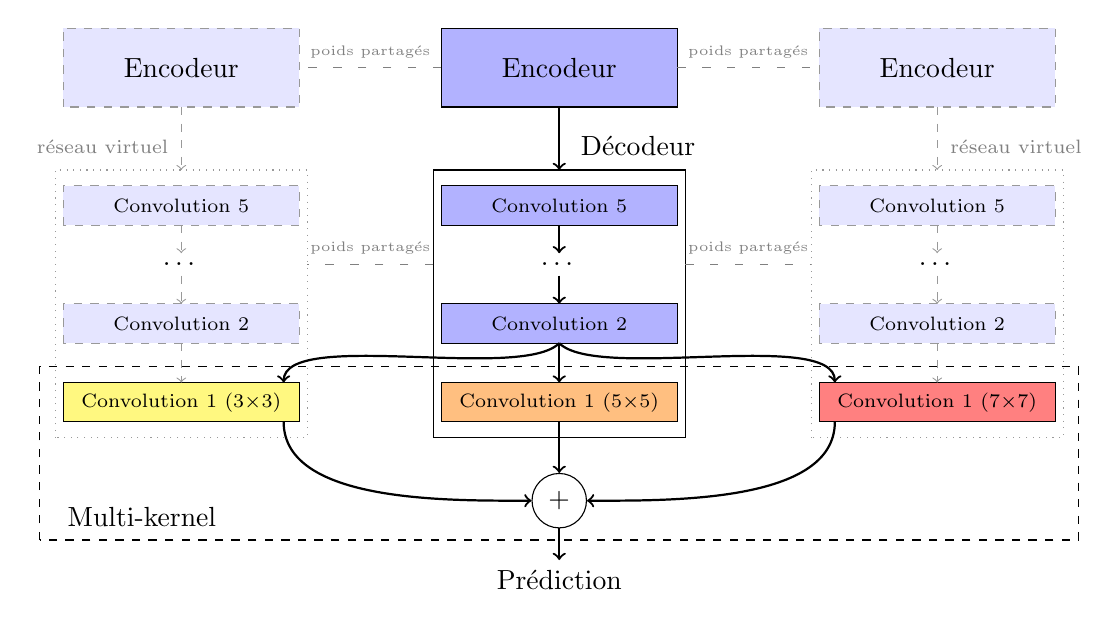
\begin{tikzpicture}[]
	\def \width {4}

     \def\colblue{blue!30!white};
     \newcommand\convblock[4]{%{x}{y}{texte}{style}
     \fill[#4]  (#1,#2) rectangle node[] {\scriptsize #3} (3+#1, 0.5+#2);
     }

     \fill[draw=black,fill=\colblue]  (-1.5,-0.5) rectangle node[black] {Encodeur} (1.5,0.5);
     \convblock{-1.5}{-2}{Convolution 5}{draw=black,fill=\colblue};
     \node (dots) at (0,-2.5) {\dots};
     \convblock{-1.5}{-3.5}{Convolution 2}{draw=black,fill=\colblue};
     \node at (1, -1) {Décodeur};
     \draw[] (-1.6, -4.7)  rectangle (1.6, -1.3);
     \convblock{-1.5}{-4.5}{Convolution 1 (5$\times$5)}{draw=black,fill=orange!50};
     \draw[thick,->] (0,-0.5) -- (0,-1.3);
     \draw[thick,->] (0, -2) -- (dots.north);
     \draw[thick,->] (dots.south) -- (0,-3);
     \draw[thick,->] (0,-3.5) -- (0, -4);

     \def\leftx{-4.8}
     \fill[draw=black!40,dashed,fill=blue!10]  (-1.5+\leftx,-0.5) rectangle node[black] {Encodeur} (1.5+\leftx,0.5);
     \convblock{-1.5+\leftx}{-2}{Convolution 5}{draw=black!40,fill=blue!10,dashed};
     \node (dots) at (\leftx,-2.5) {\dots};
     \convblock{-1.5+\leftx}{-3.5}{Convolution 2}{draw=black!40,fill=blue!10,dashed};
     \draw[dotted,black!40] (-1.6+\leftx, -4.7) rectangle (1.6+\leftx, -1.3);
     \convblock{-1.5+\leftx}{-4.5}{Convolution 1 (3$\times$3)}{draw=black,fill=yellow!50};
     \draw[->,dashed,black!40] (\leftx,-0.5) -- (\leftx,-1.3);
     \draw[->,dashed,black!40] (\leftx, -2) -- (dots.north);
     \draw[->,dashed,black!40] (dots.south) -- (\leftx,-3.);
     \draw[->,dashed,black!40] (\leftx,-3.5) -- (\leftx, -4);
     \node at (\leftx-1, -1) {\scriptsize \color{gray} réseau virtuel};
     \draw[draw=gray,loosely dashed] (-1.5,0) -- node[above] {\color{gray} \tiny poids partagés} (+1.5+\leftx,0);
     \draw[draw=gray,loosely dashed] (-1.6,-2.5) -- node[above] {\color{gray} \tiny poids partagés} (+1.6+\leftx,-2.5);

     \def\leftx{4.8}
     \fill[draw=black!40,dashed,fill=blue!10]  (-1.5+\leftx,-0.5) rectangle node[black] {Encodeur} (1.5+\leftx,0.5);
     \convblock{-1.5+\leftx}{-2}{Convolution 5}{draw=black!40,fill=blue!10,dashed};
     \node (dots) at (\leftx,-2.5) {\dots};
     \convblock{-1.5+\leftx}{-3.5}{Convolution 2}{draw=black!40,fill=blue!10,dashed};
     \draw[dotted,black!40] (-1.6+\leftx, -4.7) rectangle (1.6+\leftx, -1.3);
     \convblock{-1.5+\leftx}{-4.5}{Convolution 1 (7$\times$7)}{draw=black,fill=red!50};
     \draw[->,dashed,black!40] (\leftx,-0.5) -- (\leftx,-1.3);
     \draw[->,dashed,black!40] (\leftx, -2) -- (dots.north);
     \draw[->,dashed,black!40] (dots.south) -- (\leftx,-3.);
     \draw[->,dashed,black!40] (\leftx,-3.5) -- (\leftx, -4);
     \node at (\leftx+1, -1) {\scriptsize \color{gray} réseau virtuel};
     \draw[draw=gray,loosely dashed] (1.5,0) -- node[above] {\color{gray} \tiny poids partagés} (-1.5+\leftx,0);
     \draw[draw=gray,loosely dashed] (1.6,-2.5) -- node[above] {\color{gray} \tiny poids partagés} (-1.6+\leftx,-2.5);

     \node[draw=black,circle] (+) at (0,-5.5) {+};
     \draw[dashed] (-1.8-\leftx, -6) rectangle (1.8+\leftx, -3.8);

     \draw (0, -3.5) edge[thick,->,out=-45,in=90,looseness=0.5] (3.5,-4);
     \draw (0, -3.5) edge[thick,->,out=225,in=90,looseness=0.5] (-3.5,-4);

     \draw (0, -4.5) edge[thick,->] (+.north);
     \draw (-3.5, -4.5) edge[thick,->,in=180,out=270,looseness=0.8] (+.west);
     \draw (3.5, -4.5) edge[thick,->,in=0,out=270,looseness=0.8] (+.east);

     \node at (-5.3, -5.7) {Multi-kernel};
     \node (out) at (0, -6.5) {Prédiction};
     \draw[thick,->] (+.south) to (out.north);
\end{tikzpicture}
\end{document}
}
  \caption{Une dernière couche convolutive opérant sur 3 voisinages spatiaux différents est équivalent à moyenner 3 modèles aux poids partagés.}
  \label{fig:contextual_module}
  %\vspace*{-1em}
\end{figure}

Les approches convolutives multi-échelles ont montré à plusieurs reprises leur utilité pour la reconnaissance d'objets dans les réseaux Inception~\cite{szegedy_going_2015} et pour la segmentation sémantique~\cite{yu_multi-scale_2015}, y compris en télédétection~\cite{zhao_learning_2016}. Nous proposons ici de modifier la dernière couche du décodeur de SegNet pour extraire plusieurs cartes d'activation prenant en compte différentes tailles de contexte spatial. En particulier, nous proposons d'utiliser non pas un unique noyau convolutif $3\times3$, mais un ensemble de convolutions $3\times3$, $5\times5$ et $7\times7$ opérant en parallèle. En pratique, ceci correspond à créer un ensemble de trois modèles partageant la même topologie et les mêmes poids, à l'exception de la dernière couche, comme illustré dans la \cref{fig:contextual_module}. En notant $X_p$ les activations entrant dans la couche à plusieurs noyaux, $Z_p^s$ les activations en sortie à l'échelle $s$ ($s \in \{ 1, \dots, S \}$ avec $S = 3$), $Z'_q$ les sorties finales et $W_{p,q}^s$ le $q$\ieme noyau de convolution pour l'entrée $p$ à l'échelle $s$ :

\begin{equation}
Z'_q = \frac{1}{S} \sum_{s=1}^S Z_p^s = \frac{1}{S} \sum_{s=1}^S \sum_p W_{p,q}^s X_p~.
\end{equation}

Pour un pixel à l'indice $i$ d'activation $z_{k}^{s,i}$ pour la classe $k$ et l'échelle $s$, l'entropie croisée après \emph{softmax} est obtenue par :
\begin{equation}
\mathcal{L}(z,y) = \sum_{i=1}^N \sum_{j=1}^{k} y_j^i \log\left(\frac{\exp(\frac{1}{S} \sum\limits_{s=1}^S {z_{j}^{s,i}})}{\sum\limits_{l=1}^k \exp(\frac{1}{S} \sum\limits_{s=1}^S{z_{l}^{s,i}})}\right)~.
\end{equation}

S'il est possible d'entraîner le modèle en un seul bloc, il est toutefois plus flexible d'ajouter \emph{a posteriori} des noyaux de convolution supplémentaires. Initialement, le réseau est entraîné sur une seule échelle. Après entraînement, il est possible de remplacer la dernière convolution par une autre avec un noyau plus petit ou plus grand, sur lequel on réalise un \emph{fine-tuning}. Le noyau ainsi appris peut alors être ajouté à la dernière couche afin d'obtenir deux branches parallèle, et ainsi de suite.

Cette approche multi-kernel se rapproche des blocs Inception~\cite{szegedy_going_2015} et de la convolution compétitive multi-échelles de~\citet{liao_competitive_2015}. Cependant, ici seule la dernière couche comporte plusieurs noyaux convolutifs et le nombre de noyaux parallèles peut aisément être modifié après optimisation du modèle si la taille des objets d'intérêt vient à changer. Cette approche se retrouve dans le principe de l'agrégation de contextes de~\citet{yu_multi-scale_2015} utilisant des convolutions dilatées, permettant d'extraire des caractéristiques à plusieurs échelles. Toutefois, ici nous nous focalisons sur l'extraction de plusieurs tailles de contextes à une échelle locale et écartons la convolution à trous, coûteuse en temps de calcul, ou l'utilisation d'une pyramide d'images multi-échelles~\cite{zhao_learning_2016}. Nous proposons donc s'agit une plus méthode simple et plus flexible pour agréger des prédictions sur plusieurs contextes spatiaux à partir d'un extracteur de caractéristiques fixe.

\subsubsection{Supervision profonde}
\label{sec:deep_multiscale}

Le traitement multi-échelles des images de télédétection est généralement effectuée en utilisant une approche pyramidale : différents contextes à différentes résolutions sont fournis comme entrées à un ou plusieurs classifieurs. Nous proposons ici d'utiliser une approche alternative consistant à n'en traiter qu'une seule mais à produire en sortie du \gls{FCN} une pyramide de prédictions, comme introduit dans le modèle DeepLab~\cite{l._c._chen_deeplab_2018}. Chaque sortie est une carte prédite à une résolution différente sur laquelle il est possible de calculer une erreur qui sera rétropropagée dans le réseau. Ceci permet de réaliser d'une part une inférence multi-échelles et d'autre part d'introduire une forme de supervision profonde dans le modèle~\cite{lee_deeply-supervised_2015}.

Dans le modèle SegNet, la pyramide de cartes d'activations apparaît naturellement dans le décodeur. Après le $p$\ieme bloc du décodeur, nous ajoutons une couche convolutive réalisant une classification à la résolution $\frac{2^p W}{32} \times \frac{2^p H}{32}$, comme illustré dans la~\cref{fig:ms_deep_segnet}. Ces cartes sont ensuite interpolées à la résolution $W\times H$ et sommées pour obtenir la carte sémantique finale. En notant $P_{\mathit{compl\grave{e}te}}$ la prédiction à pleine résolution, $P_{\mathit{r\acute{e}duite}_d}$ les cartes obtenues avec un facteur d'échelle $1:d$ et $\mathcal{I}_d$ l'interpolation bilinéaire d'un facteur $d$, la carte complète est obtenue par\,:
\begin{equation}
P_{\mathit{compl\grave{e}te}} = \sum_{d \in \{0, 2, 4, 8\}} \mathcal{I}_d(P_{\mathit{r\acute{e}duite}_d}) = P_0 + \mathcal{I}_2(P_2) + \mathcal{I}_4(P_4) + \mathcal{I}_8(P_8).
\end{equation}

Lors de la rétropropagation, chaque bloc convolutif du décodeur reçoit deux gradients\,:
\begin{itemize}
	\item Un gradient correspondant à la fonction de coût finale,
  \item Un gradient correspondant à la fonction de coût réduite.
\end{itemize}
Les couches les plus profondes peuvent ainsi simplement apprendre à raffiner les prédictions de la couche précédente, ce qui simplifie l'optimisation globale du réseau~\cite{lin_refinenet_2016}.

\section{Évaluation des modèles}

\subsection{Métriques pour la classification}

\def\tp{V^+}
\def\tn{V^-}
\def\fp{F^+}
\def\fn{F^-}

\begin{figure}
	\resizebox{\textwidth}{!}{%
	\documentclass{standalone}
\usepackage[utf8]{inputenc}
\usepackage[T1]{fontenc}
\usepackage{tikz}
%%%%%%%%%%%%%%%%%%%%%%%%%%%%%%%%%%%%%%%%
%           Commandes perso            %
%%%%%%%%%%%%%%%%%%%%%%%%%%%%%%%%%%%%%%%%

%% Figures centrées, et en position 'here, top, bottom or page'
\newenvironment{figureth}{%
		\begin{figure}[htbp]
			\centering
	}{
		\end{figure}
		}


%% Tableaux centrés, et en position 'here, top, bottom or page'
\newenvironment{tableth}{%
		\begin{table}[htbp]
			\centering
			%\rowcolors{1}{coleurtableau}{coleurtableau}
	}{
		\end{table}
		}

%% Sous-figures centrées, en position 'top'
\newenvironment{subfigureth}[1]{%
	\begin{subfigure}[t]{#1}
	\centering
}{
	\end{subfigure}
}

\newcommand{\citationChap}[2]{%
	\epigraph{\og \textit{#1} \fg{}}{#2}
}

%% On commence par une page impaire quand on change le style de numérotation de pages
\let\oldpagenumbering\pagenumbering
\renewcommand{\pagenumbering}[1]{%
	\cleardoublepage
	\oldpagenumbering{#1}
}

%% Légende du dataset ISPRS
\newcommand\isprslegende{
Légende\,: \textcolor{Black}{blanc}\,: routes, \textcolor{Blue}{bleu}\,: bâtiments, \textcolor{Cerulean}{cyan}\,: végétation basse, \textcolor{OliveGreen}{vert}\,: arbres, \textcolor{Dandelion}{jaune}\,: véhicules, \textcolor{BrickRed}{rouge}\,: autre.
}

%% Dessiner des réseaux de neurones avec Tikz
\newcommand{\convlayer}[9]{%{h}{w}{d}{name}{color}{x}{y}{z}%{note w}{note h}{note d}
   \def\h{#1}
   \def\w{#2}
   \def\d{#3}
   \def\name{#4}
   \ifthenelse {\equal{#5} {}} {\def\col{white}} {\def\col{#5}}
   \def\x{#6}
   \ifthenelse {\equal{#7} {}} {\def\y{0}} {\def\y{#7}}
   \ifthenelse {\equal{#8} {}} {\def\z{0}} {\def\z{#8}}
   % ne faites pas ça chez vous !
   \ifthenelse {\equal{#9} {}} {\convlayercontinued{}{}{}} {\convlayercontinued#9}
}

\newcommand\convlayercontinued[3]{
   \def\notew{#1}
   \def\noteh{#2}
   \def\noted{#3}
   \coordinate (A) at (\x-\d/2,  \y-\h/2, \z-\w/2);
   \coordinate (B) at (\x-\d/2,  \y-\h/2, \z+\w/2);
   \coordinate (C) at (\x-\d/2,  \y+\h/2, \z+\w/2);
   \coordinate (D) at (\x-\d/2,  \y+\h/2, \z-\w/2);
   \coordinate (E) at (\x+\d/2,  \y-\h/2, \z-\w/2);
   \coordinate (F) at (\x+\d/2,  \y-\h/2, \z+\w/2);
   \coordinate (G) at (\x+\d/2,  \y+\h/2, \z+\w/2);
   \coordinate (H) at (\x+\d/2,  \y+\h/2, \z-\w/2);

    \draw [draw opacity=0.3, fill opacity=0.8, fill=\col!60!white] (A) -- (B) -- (C) -- (D) -- cycle;
    \draw [draw opacity=0.3, fill opacity=0.8, fill=\col!60!white] (A) -- (B) -- (F) -- (E) -- cycle;
    % Face haut
    %\draw [left color=\col!60!white, right color=\col!80!white, shading=axis, shading angle=180] (C) -- (D)  -- (H) -- (G) -- cycle;
    \draw [fill opacity=0.9, fill=\col!70!white] (C) -- node[rotate=45,above] {\small \name} (D) -- (H) -- (G) -- cycle;
    %\draw [fill opacity=0.9, fill=\col!70!white] (C) -- (D) -- node[above] {\small \name} (H) -- (G) -- cycle;
    % Face droite
    \draw [fill opacity=0.9, fill=\col!60!white] (E) -- node[pos=0.75,rotate=45,below] {\scriptsize \notew} (F) -- (G) --  (H) -- cycle;
    % Face avant
    %\draw [shading=axis, left color=\col!60!white, right color=\col!40!white, shading angle=-45] (B) -- node[above,rotate=90] {\scriptsize \noteh} (C) -- (G) -- (F) -- node[below] {\scriptsize \noted}  cycle;
    \draw [fill opacity=0.9, fill=\col!50!white] (B) -- node[above,rotate=90] {\scriptsize \noteh} (C) -- (G) -- (F) -- node[below] {\scriptsize \noted}  cycle;
}

\newcommand{\fclayer}[8]{%{h}{w}{name}{color}{x}{y}{z}
   \def\h{#1}
   \def\w{#2}
   \def\name{#3}
   \ifthenelse {\equal{#4} {}} {\def\col{white}} {\def\col{#4}}
   \def\x{#5}
   \def\y{#6}
   \def\z{#7}
   \def\note{#8}
   \coordinate (A) at (\x-\w/2,  \y-\h/2, \z);
   \coordinate (B) at (\x+\w/2,  \y-\h/2, \z);
   \coordinate (C) at (\x+\w/2,  \y+\h/2, \z);
   \coordinate (D) at (\x-\w/2,  \y+\h/2, \z);

   \pgfmathparse{4*\w}\let\boxwidth\pgfmathresult
    \draw [fill=\col] (A) -- node[below,text width=\boxwidth cm,align=center] {\scriptsize \note} (B) -- (C) -- (D) -- cycle;

    \node (N) at ($(A)!0.5!(B)+(0,-1,0)$) {\name};
}

\newcommand{\alexnet}[4]{%{scale}{x}{y}{z}
  \def\scale{#1}
  \def\alexx{#2}
  \def\alexy{#3}
  \def\alexz{#4}


  \def\coblue{blue!50!white}
  \def\fcgrey{gray!50!white}

  \convlayer{1.3*\scale}{1.3*\scale}{0.02*\scale}{Image}{\coblue}{\alexx}{\alexy}{\alexz}{{227}{227}{3}}
  \convlayer{1.1*\scale}{1.1*\scale}{0.08*\scale}{Conv1}{\coblue}{\alexx+0.7*\scale}{\alexy}{\alexz}{{55}{55}{96}}
  \convlayer{0.7*\scale}{0.7*\scale}{0.5*\scale}{Conv2}{\coblue}{\alexx+1.5*\scale}{\alexy}{\alexz}{{27}{27}{256}}
  \convlayer{0.5*\scale}{0.5*\scale}{0.8*\scale}{Conv3}{\coblue}{\alexx+2.6*\scale}{\alexy}{\alexz}{{13}{13}{384}}
  \convlayer{0.5*\scale}{0.5*\scale}{0.8*\scale}{Conv4}{\coblue}{\alexx+3.8*\scale}{\alexy}{\alexz}{{13}{13}{384}}
  \convlayer{0.5*\scale}{0.5*\scale}{0.5*\scale}{Conv5}{\coblue}{\alexx+4.8*\scale}{\alexy}{\alexz}{{13}{13}{256}}
  \fclayer{\scale}{0.1*\scale}{FC1}{\fcgrey}{\alexx+5.4*\scale}{\alexy}{\alexz}{4096}
  \fclayer{\scale}{0.1*\scale}{FC2}{\fcgrey}{\alexx+5.7*\scale}{\alexy}{\alexz}{4096}
  \fclayer{\scale}{0.1*\scale}{FC3}{\fcgrey}{\alexx+6.0*\scale}{\alexy}{\alexz}{1000}
}

\newcommand{\imagelayer}[7]{%{width}{x}{y}{z}{path}{text_up}{text_down}
    \pgfmathparse{#1}\let\w\pgfmathresult
    \begin{scope}[canvas is yz plane at x=#2]
     \node[transform shape] (source) at (#3, #4) {\includegraphics[angle=-90,width=\w cm]{#5}};
    \end{scope}
     \node [transform shape, rotate=45, above] at (source.east) {#6};
     \node [transform shape, rotate=45, below] at (source.west) {\scriptsize{#7}};
}

\def\fourier{\mathcal{F}}

\newcommand{\lightspectrum}{%
\pgfplotsset{
    % this *defines* a custom colormap ...
    colormap={slategraywhite}{color(0cm)=(red); color(1cm)=(red); color(2cm)=(red); color(3cm)=(red); color(4cm)=(orange); color(5cm)=(yellow); color(6cm)=(green); color(7cm)=(blue); color(8cm)=(blue); color(9cm)=(purple); color(10cm)=(purple); color(12cm)=(black)}
}
\node at (1.5, 2.7) {\small 1mm};
\node at (4, 3) {Infrarouge};
\node at (7.75, 2.7) {\small 800nm};
\node at (9, 3) {Visible};
\node at (10.5, 2.7) {\small 400nm};
\node at (12, 3) {Ultraviolet};
\node at (13.5, 2.7) {\small 10nm};
\draw[->] (1, 2.5) -- (14, 2.5);
\begin{axis}[hide axis,width=16cm,height=4cm,colormap name=slategraywhite]
\addplot[domain=20:1000,samples=1500,ultra thick, point meta=x*x,mesh]{sin(x*x/80)};
\end{axis}
}

% Union généralisée
\newcommand{\wbigcup}{\mathop{\bigcup}\displaylimits}

\newcommand{\res}[2]{#1 {\footnotesize $\pm$ #2}}
\newcommand{\bres}[2]{\textbf{#1} {\footnotesize $\pm$ #2}}
\newcommand{\bbres}[2]{\res{\textit{#1}}{#2}}

\newcommand{\drawkernel}[9]{
\begin{tikzpicture}
	\draw[step=1cm,gray!50!white,very thin] (0,0) grid (3,3);
	\kernelnode{0.5}{0.5}{#1};
	\kernelnode{0.5}{1.5}{#2};
	\kernelnode{0.5}{2.5}{#3};
	\kernelnode{1.5}{0.5}{#4};
	\kernelnode{1.5}{1.5}{#5};
	\kernelnode{1.5}{2.5}{#6};
	\kernelnode{2.5}{0.5}{#7};
	\kernelnode{2.5}{1.5}{#8};
	\kernelnode{2.5}{2.5}{#9};
\end{tikzpicture}
}

\newcommand{\kernelnode}[3]{%{x}{y}{value}
	\ifthenelse{\equal{#3}{0}}{
		\def\kcolor{gray}
	}{
		\def\kcolor{black}
	}
	\node[\kcolor] at (#1, #2) {#3};
}

\newcommand{\chapsummary}[1]{
\section*{Résumé du chapitre :}
\parbox{0.9\linewidth}{
\setlength{\parindent}{4ex}
#1}
}

\newcommand{\eqname}[1]{\tag*{\small (#1)}}

\begin{document}

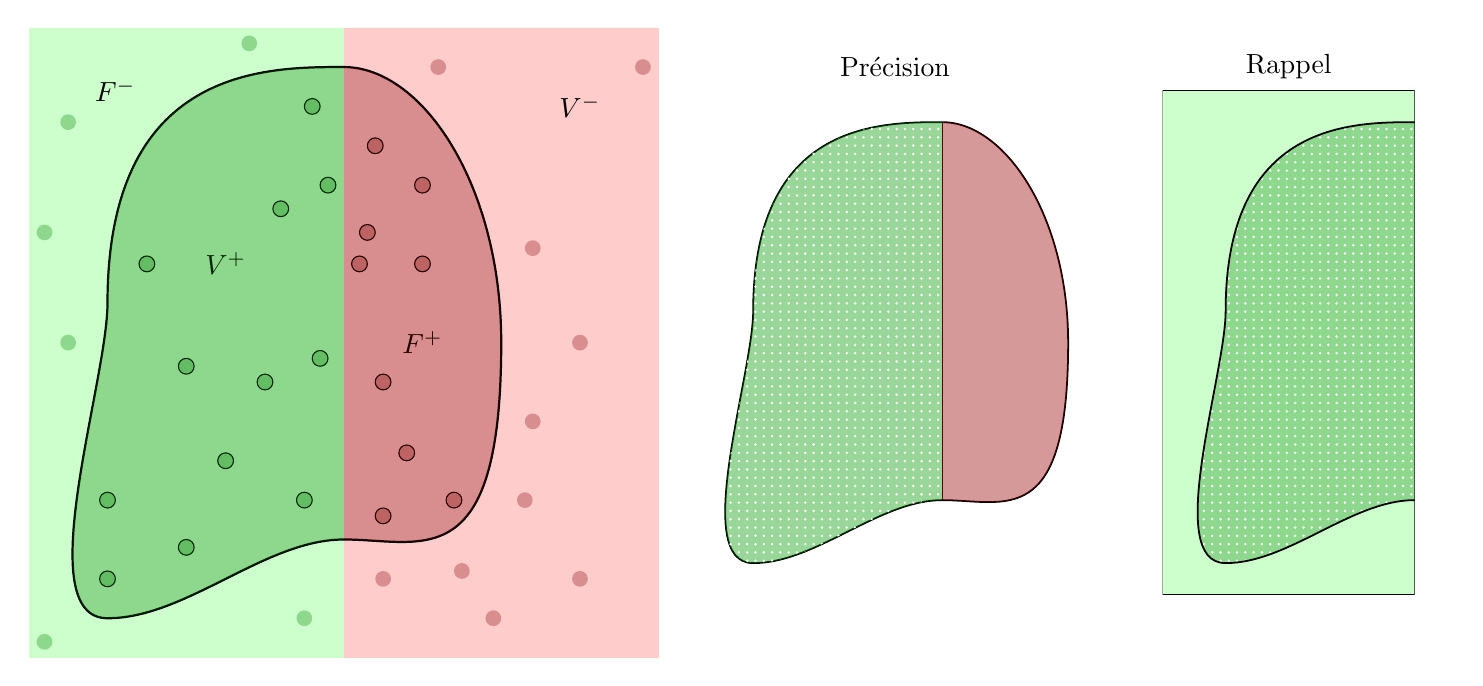
\begin{tikzpicture}
\usetikzlibrary{patterns}
\newcommand\patatoid{(-3,-3.5) .. controls +(1,0) and +(-1,0) .. (0,-2.5) 
             .. controls +(1,0) and +(0,-3) .. (2,0)
             .. controls +(0,2) and +(1,0)  .. (0,3.5)
             .. controls +(-1,0) and +(0,3) .. (-3,0.5)
             .. controls +(0,-1) and +(-1,0).. (-3,-3.5)}
\newcommand\positifs{(-4,-4) rectangle (0, 4)};
\newcommand\negatifs{(4,4) rectangle (0,-4)};

\fill[fill=green, opacity=0.2] \positifs;
\fill[fill=red, opacity=0.2] \negatifs;
%\draw (0,0) circle (3);


\draw[thick] \patatoid;

\foreach \x\y in {-3/-3,-1/-0.5,-2/-0.3,-2.5/1,-0.2/2,-0.3/-0.2,-0.5/-2,-0.4/3,-3/-2,-2/-2.6,-1.5/-1.5,-0.8/1.7}{
\filldraw[fill=green!50!black, opacity=0.3, draw opacity=1] (\x,\y) circle (0.1);
}

\foreach \x\y in {-3.5/2.8,-3.5/0,-0.5/-3.5,-1.2/3.8,-3.8/1.4,-3.8/-3.8}{
\fill[fill=green!50!black, opacity=0.3] (\x,\y) circle (0.1);
}

\foreach \x\y in {0.2/1,0.3/1.4,0.8/-1.4,1/2,0.4/2.5,1.4/-2,0.5/-2.2,0.5/-0.5,}{
\filldraw[fill=red!50!black, opacity=0.3, draw opacity=1] (\x,\y) circle (0.1);
}

\foreach \x\y in {3.8/3.5,3/0,2.4/1.2,2.4/-1,1.9/-3.5,3/-3,2.3/-2,0.5/-3,1.5/-2.9,1.2/3.5}{
\fill[fill=red!50!black, opacity=0.3] (\x,\y) circle (0.1);
}

\node at (3,3) {$V^-$};
\node at (1,0) {$F^+$};
\node at (-1.5,1) {$V^+$};
\node at (-2.9, 3.2) {$F^-$};

\begin{scope}[]
\clip  \positifs;
\fill[green!50!black,opacity=0.3] \patatoid;
\end{scope}
\begin{scope}[]
\clip  \negatifs;
\fill[red!50!black,opacity=0.3] \patatoid;
\end{scope}

\begin{scope}[xshift=9.5cm,transform canvas={scale=0.8}]
\draw[thick] \patatoid;
\clip \patatoid;
\filldraw[preaction={fill, green!60!black, opacity=0.4}, opacity=1, pattern=dots, pattern color=white] \positifs;
\filldraw[red!60!black,opacity=0.4] \negatifs;
\end{scope}
\node at (7,3.5) {Précision};

\begin{scope}[xshift=17cm, transform canvas={scale=0.8}]
\clip  \positifs;
\filldraw[green,opacity=0.2,draw=black,draw opacity=1] \positifs;
\filldraw[preaction={fill=green!50!black,fill opacity=0.3}, pattern=dots, opacity=1, pattern color=white,thick] \patatoid;
\end{scope}
\node at (12,3.5) {Rappel};

\node at (14,0) {};

\end{tikzpicture}
\end{document}

	}
	\caption{Répartition des vrais positifs $\tp$, des vrais négatifs $\tn$, des faux positifs $\fp$ et des faux négatifs $\fn$ pour une classification binaire dans un espace à deux dimensions.}
	\label{fig:classification_binaire}
\end{figure}

Pour un classifieur donné et une classe d'intérêt $i$, on définit $\tp$ comme l'ensemble des vrais positifs(échantillons appartenant à la classe $i$ correctement affectés), $\tn$ l'ensemble des vrais négatifs (échantillons à une classe $j \neq i$ n'étant pas affectés à $i$), $\fp$ l'ensemble des faux positifs (échantillons d'une classe $j \neq i$ ayant été affectés $i$) et $\fn$ l'ensemble des faux négatifs (échantillons de $i$ affectés $j \neq i$). Ce partionnement est illustré dans la~\cref{fig:classification_binaire}.

On définit alors les métriques de performance suivantes pour le classifieur, relativement à la classe $i$:
\begin{itemize}
	\item La précision est définie comme le rapport entre le nombre de vrais positifs et le nombre total d'éléments affectés à la classe par le classifieur\,:
  $$pr\acute{e}cision = \frac{\tp}{\tp + \fp}~.$$
	\item Le rappel est défini comme le rapport entre le nombre de vrais positifs et le nombre total d'éléments appartenant réellement à la classe\,:
  $$rappel = \frac{\tp}{\tp + \fn}~.$$
	\item Le score $F_1$, ou c\oe{}fficient de Sorensen-Dice, est défini comme la moyenne harmonique de la précision et du rappel\,:
  $$F_1 = 2~.~\frac{pr\acute{e}cision \times rappel}{pr\acute{e}cision + rappel}~,$$
  ce qui s'écrit également\,:
  $$F_1 = \frac{2 \tp}{2 \tp + \fp + \fn}~.$$
	\item L'exactitude est définie comme le rapport de prédictions exactes sur le nombre total d'échantillons\,:
  $$Exactitude = \frac{\tp + \tn}{\tp + \fp + \tn + \fn}~.$$
	\item L'\gls{IsU}, ou indice de Jaccard, est définie comme le rapport du nombre de prédictions exactes sur l'ensemble des prédictions de la classe et des échantillons réels\,:
  $$\glsname{IsU} = \frac{\tp}{\tp + \fp + \fn}~.$$
\end{itemize}

Le score $F_1$ et l'\gls{IsU} ont l'avantage de ne pas être biaisé en faveur d'une classe dominante. Par exemple, un jeu de données contenant 95\% de fond et 5\% d'objet sera classifié à 95\% d'exactitude par un classifieur prédisant systématiquement ``fond''. Cependant, le score $F_1$ de ce classifieur ne serait que serait $0$.

L'\gls{IsU} est proche du score $F_1$, mais accorde une pondération plus importante aux vrais positifs. Toutefois, les deux métriques peuvent être utilisées pour ordonner des classifieurs. Étant donné que $\gls{IsU}/F = 1/2 + \gls{IsU}/2$, il existe un relation monotone entre les deux métriques. Un classifieur $A$ meilleur qu'un classifieur $B$ pour l\gls{IsU} le sera également pour le score $F_1$, et réciproquement.

Dans un cadre multi-classe, on s'intéressera à l'exactitude globale et la moyenne de l'intersection sur union ou la moyenne du score $F_1$ sur l'ensemble des classes.

\subsection{Métriques pour la segmentation}

Dans un premier temps, il s'agit d'évaluer les capacités théoriques des différents algorithmes de pré-segmentation. En effet, si la segmentation rassemble dans une même région des pixels appartenant à deux classes différentes, il apparaîtra nécessairement des erreurs dans la classification finale, car une région ne sera associée qu'à une unique classe.

De fait, nous pouvons comparer les algorithmes de segmentation sur les images de la base selon trois critères\,:
\begin{itemize}
  \item L'erreur de sous-segmentation (ESS), définie comme le ratio de pixels appartenant à une région qui en recouvrent une autre. Formellement, si $S$, $P$ et $N$ sont respectivement les régions réelles, les régions issues de la segmentation et le nombre de pixels dans l'image\,:
  $$ESS = \frac{1}{N} \sum_{S \in GT} \sum_{P : P \cap S \neq \emptyset} min(|P \cap S|, |P \backslash P \cap S|)$$
  \item Le rappel sur les bordures (RB), défini comme le rappel statistique des pixels placés à la frontière des segments qui se trouvent dans un 3-voisinage des frontières réelles\,:
  $$RB =  \frac{true\ pos.}{true\ pos. + false\ neg.}$$
  \item La pureté moyenne (PM), définie comme le pourcentage moyen de pixels d'un segment appartenant à la région sous-jacente la plus représentée. En notant $moy$ et $maj$ la fonction de calcul de moyenne et l'identifiant de la région majoritaire\,:
  $$PM = \underset{P \in seg}{moy} \left(\frac{| P \cap maj(P)|}{| P |}\right)$$
  \item L'oracle, défini comme le taux de bonne classification pixellique qui serait obtenu par un classifieur parfait, assignant la classe majoritaire à chaque segment. Il s'agit de la meilleure classification possible théoriquement obtensible avec la segmentation considérée.
\end{itemize}

\subsection{Classification par région}
\label{sec:results_region}

Nous choisissons d'évaluer différents algorithmes de segmentation non-supervisé dans un cadre de classification par région sur le jeu de données \gls{ISPRS} 2D \emph{Semantic Labeling} Vaihingen. Celui comporte une acquisition aérienne \gls{EHR} de la ville allemande de Vaihingen sur les canaux \gls{IRRV} et est annoté dans 6 classes d'intérêt. Le jeu de données précis est détaillé dans l'\cref{annexe:isprs}.

Nous comparons les algorithmes de segmentation les plus couramment utilisés dans la communauté vision par ordinateur et dans la communauté télédétection, identifiés dans la~\cref{sec:segmentations}\,: \gls{SLIC}, \gls{LSC}, Quickshift, \gls{MRS} (eCognition\copyright) et \gls{HSEG}. Les paramètres des segmentations sont réglés afin d'obtenir un nombre de régions similaire et les meilleures performances possibles. Ces algorithmes de segmentation sont représentatifs des grandes familles d'algorithmes qu'il est raisonnable d'utiliser pour une classification par région.

\begin{table}
  \centering
  \setlength{\tabcolsep}{10pt}
  \begin{tabularx}{\textwidth}{ Y c c c c c }
  \toprule
  Algorithme & Nombre de régions & ESS (\%) & RB (\%) & PM (\%) & Oracle (\%)\\
  \midrule
  \gls{SLIC} & \textbf{20 000} & \textbf{10.21} & 84.07 & 75.10 & 89.91\\
  \gls{LSC} & 22 800 & 11.37 & 91.13 & 71.54 & 85.83\\
  Quickshift & 21 000 & 11.66 & 88.34 & 72.90 & 83.61\\
  \cmidrule(lr){1-6}
  \gls{MRS} & 23 500 & 13.12 & \textbf{95.71} & \textbf{79.08} & \textbf{91.68}\\
  \gls{HSEG} & 21 000 & 11.39 & 94.83 & 78.66 & 85.25\\
  \bottomrule
  \end{tabularx}
  \caption{Métriques de comparaison des algorithmes de segmentation sur le jeu de données \gls{ISPRS} Vaihingen.}
  \label{table:segmentation_metrics}
\end{table}

\begin{table}
  \begin{tabularx}{\textwidth}{ Y c c c c c }
  \toprule
  Algorithme & Nombre de régions & Exactitude (\%) & Score $F_1$ (véhicules) & $\kappa$ & Oracle (\%)\\
	\midrule
  \gls{SLIC} & $\simeq$\textbf{20 000} & 82.20 & 0.54 & 0.76 & 89.91\\
  \gls{LSC} & $\simeq$22 800 & \textbf{82.45} & \textbf{0.58} & 0.76 & 85.53\\
  Quickshift & $\simeq$21 000 & 82.05 & 0.52 & 0.75 & 93.61\\
  \cmidrule(lr){1-5}
  \gls{MRS} & $\simeq$23 500 & 80.53 & 0.56 & 0.73 & \textbf{91.68}\\
  \gls{HSEG} & $\simeq$21 000 & 79.56 & 0.54 & 0.72 & 85.25\\
  \cmidrule(lr){1-5}
  Fenêtre glissante & $\simeq$23 800 & 81.22 & 0.53 & 0.74 & 92.56\\
  \bottomrule
  \end{tabularx}
  \caption{Résultats de classification sur le jeu de données \gls{ISPRS} Vaihingen.}
  \label{table:classification_metrics}
\end{table}

Nous appliquons ces algorithmes de segmentation sur l'ensemble des images du jeu de données \gls{ISPRS} Vaihigen. Nous utilisons l'implémentation des auteurs pour \gls{LSC}~\cite{li_superpixel_2015}, l'implémentation de~\citet{guyet_extraction_2015} de l'algorithme \gls{MRS} (adapté depuis la bibliothèque TerraLib~\cite{camara_terralib_2008}) et les implémentations de la bibliothèque scikit-image~\cite{walt_scikit-image_2014} pour \gls{SLIC} et \emph{Quickshift}.
Les résultats sont détaillés dans le tableau~\cref{table:segmentation_metrics}.

Tout d'abord, on constate que l'algorithme \gls{MRS} présente un rappel sur les bordures très élevé, ce qui signifie que les frontières définie par cette segmentation sont proches des véritables bordures. Cela correspond à ce qu'il est visuellement possible d'observer\,: \gls{MRS} privilégie des régions très homogènes, quitte à les rendre très irrégulières. Cela bénéficie en outre au critère de pureté qui en est mécaniquement plus élevé. L'algorithme \gls{SLIC} semble également tirer son épingle du jeu, grâce à une faible erreur de sous-segmentation.

Dans l'ensemble, les performances théoriques de classification atteignables (oracle) varient de 83\% à 91\%.

Le~\cref{table:classification_metrics} détaille les résultats obtenus après une classification par le protocole décrit précédemment. Le AlexNet extracteur de caractéristiques est implémenté en utilisant la bibliothèque d'apprentissage profond Caffe~\cite{jia_caffe_2014}. Le classifieur utilisé est une \gls{SVM} linéaire optimisée par descente de gradient telle qu'implémentée dans la bilbiothèque scikit-learn~\cite{pedregosa_scikit-learn_2011}.
Il s'avère que le classement par taux de bonne classification ne correspond pas au classement utilisant l'oracle comme mesure. Cela signifie que les performances brutes de segmentation ne suffisent pas à déterminer la pertinence d'une segmentation dans un cadre d'extraction de caractéristiques.

En effet, les résultats de classification poussent à privilégier des approches de type superpixels. La régularité géométrique des segments bénéficie grandement au classifieur. Les segments présentent tous une compacité et une convexité forte. Au moment de l'extraction de l'imagette, la majorité des pixels au centre de l'image sont donc pertinents, et la caractéristique calculée par le réseau convolutif contiendra en grande partie de l'information issue de la région considérée. À l'inverse, les segmentations irrégulières s'imbriquent difficilement dans des imagettes rectangulaires, ce qui complexifie la tâche de classification car les échantillons d'apprentissage ne sont pas géométriquement normalisés, comme illustré par la~\cref{fig:potsdam_segmentation}. En pratique, ces segmentations n'apportent aucun gain par rapport à une simple fenêtre glissante à coût calculatoire constant.

Il est possible d'augmenter le paramètre de compacité de la segmentation \gls{MRS} pour obtenir des régions plus homogènes, visuellement proches des superpixels. Dans ce cas, les résultats sont comparables à ceux obtenus avec \gls{SLIC}, mais au prix d'une sursegmentation considérable : \gls{MRS} nécessite deux fois plus de segments que \gls{SLIC} pour le même résultat. Ceci impacte directement le temps de calcul, qui est proportionnel au nombre de régions à traiter.

Enfin, il est important de constater que les petits objets sont sensibles au choix de la pré-segmentation, comme l'analyse qualitative laissait le présager. En effet, le score $F_1$ peut être significativement amélioré par l'utilisation d'une segmentation adaptée, comme \gls{LSC}.

\subsection{Classification pixellique par segmentation sémantique}

Comme nous l'avons vu, il apparaît clairement que la mise en \oe{}uvre d'une segmentation non-supervisée est le principal facteur limitant les performances des méthodes de classification par région. En effet, non seulement l'utilisation de la segmentation réduit les performances théoriques obtenues par un oracle, mais les exemples d'apprentissage eux-mêmes ne permettent pas d'exploiter de façon satisfaisante les caractéristiques profondes. Par conséquent, il apparaît pertinent d'étudier les performances de modèles \gls{FCN} capables d'apprendre de bout en bout la segmentation et la classification.

Nous entraînons donc des modèles de réseaux profonds entièrement convolutifs SegNet et ResNet-34 sur les jeux de données \gls{ISPRS} Vaihingen et \gls{ISPRS} Potsdam.
Nous traitons chaque tuile du jeu de données par une fenêtre glissante de dimensions $128 \times 128$ et un pas variable. Les modèles sont entraînés pendant 50 000 itérations avec une taille de \emph{batch} de 10. Le taux d'apprentissage initial est fixé à 0,1 et est divisé par 10 après 35 000 et 45 000 itérations.
Les réseaux sont implémentés à l'aide des bibliothèques Caffe~\cite{jia_caffe_2014} et PyTorch~\cite{paszke_automatic_2017}.

Dans un premier temps, nous validons cette approche uniquement sur les données pour lesquelles une vérité terrain est disponible, que nous divisons en deux sous-ensembles : apprentissage et validation. Pour comparer notre méthode à l'état-de-l'art, nous entraînons ensuite notre modèle sur l'ensemble du jeu de données (apprentissage + validation) avec les mêmes hyperparamètres. Nous soumettons enfin nos résultats sur le jeu de données de test au serveur d'évaluation de l'\gls{ISPRS}, dont la vérité terrain nous est inconnue.

\subsubsection{Recouvrement de la fenêtre glissante}

\begin{table}[t]
  \centering
  \caption{Résultats sur le jeu de validation \gls{ISPRS} Vaihingen en fonction du recouvrement de la fenêtre glissante.}
  \setlength{\tabcolsep}{4pt}
  \begin{tabularx}{0.8\textwidth}{ Y c c c }
  \toprule
  Modèle/Pas (px) & 128 & 64 & 32\\
  \midrule
  SegNet \gls{IRRV} & 87,8\% & 88,3\% & 88,8\%\\
  SegNet multi-kernel & 88,2\% & 88,6\% & 89,1\%\\
  \bottomrule
  \end{tabularx}
  \label{tab:vaihingen_stride}
\end{table}

L'utilisation d'une fenêtre glissante pour la segmentation de l'image pose la question du traitement des bordures. En effet, si le pas de la fenêtre glissante est identique aux dimensions de celle-ci, il risque alors d'apparaître des discontinuités aux bordures dégradant la qualité visuelles de la segmentation. En diminuant le pas, nous pouvons autoriser un recouvrement plus ou moins important entre deux fenêtres successives, c'est-à-dire que certains pixels pourront être observés à plusieurs reprises. Ceci augmente le temps d'inférence mais accroît également la précision du modèle, comme détaillé dans le~\cref{tab:vaihingen_stride}. En effet, en divisant le pas par $2$, le nombre d'imagettes à traiter est multiplié par $4$. Cependant, moyenner plusieurs prédictions sur une même région permet de corriger des artefacts de classification, notamment le long des bords où le contexte spatial est manquant, et de lisser les discontinuités. L'expérience semble indiquer qu'un pas de $32$px (75\% de recouvrement) est suffisamment rapide pour la majorité des tâches et augmente significativement la précision (+1\%). Une tuile complète est ainsi traitée en 4 minutes sur une NVIDIA Tesla K20c avec un pas de $32$px et moins de 20 secondes avec un pas de $128$px. Nous utiliserons donc ces paramètres pour la suite de nos travaux. Dans l'ensemble, le modèle SegNet parvient à correctement classifier plus de 87\% des pixels du jeu de validation. En comparaison, aucune des méthodes de classification par région comparées précédemment ne dépassait 83\%. Notamment, SegNet parvient à dépasser les oracles sur les segmentations \gls{HSEG}, \gls{LSC} et \emph{Quickshift}. Ceci montre la pertinence des réseaux entièrement convolutifs pour la segmentation sémantique\,: inférer une classification pixellique dense contraint SegNet à apprendre conjointement des caractéristiques prenant en compte les aspects spatiaux tout en respectant au mieux la résolution de l'image.

\subsubsection{Transfert de connaissances}

\begin{table}[t]
  \centering
  \caption{Résultats des différentes stratégies d'initialisation sur le jeu de validation \gls{ISPRS} Vaihingen.}
  \begin{tabularx}{\textwidth}{ c | c | Y Y Y Y }
  \toprule
  Initialisation & Aléatoire & \multicolumn{4}{c}{VGG-16 (ImageNet)}\\
  \midrule
  Variabilité de l'encodeur $\frac{lr_{e}}{lr_{d}}$ & 1 & 1 & 0,5 & 0,1 & 0 \Snowflake\\
  \midrule
  Exactitude & 87,0\% & 87,2\% & \textbf{87,8\%} & 86,9\% & 86,5\%\\
  \bottomrule
  \end{tabularx}
  \label{tab:initialization}
\end{table}

Le pré-entraînement d'un réseau profond sur un jeu de données générique est une pratique courante pour en augmenter les capacités de généralisation. ImageNet est ainsi souvent utilisé comme base de pré-entraînement pour la plupart des tâches visuelles. La télédétection ne fait pas exception, les filtres convolutifs appris sur des images multimédia pouvant être transférés pour la classification d'images aériennes~\cite{penatti_deep_2015}. Cependant, compte-tenu des différences importantes entre ces images et celles de télédétection, il peut exister un intérêt à laisser ces filtres pré-calculés être modifiés librement lors de l'optimisation du réseau. Pour évaluer l'impact du pré-entraînement sur la classification d'images de télédétection, nous comparons différents taux d'apprentissage pour l'encodeur ($lr_{e}$) et le décodeur ($lr_{d}$) de SegNet. Nous testons notamment quatre stratégies~:
\begin{itemize}
  \item même variabilité~: $lr_{d} = lr_{e}$, ${lr_{e} / lr_{d}} = 1$,
  \item faible variabilité de l'encodeur: $lr_{d} = 2 \times lr_{e}$, ${lr_{e} / lr_{d}} = 0,5$,
  \item très faible variabilité de l'encodeur: $lr_{d} = 10 \times lr_{e}$, ${lr_{e} / lr_{d}} = 0,1$,
  \item absence de rétropropagation de l'erreur sur l'encodeur (aucune variabilité): $lr_{e} = 0$, ${lr_{e} / lr_{d}} = 0$.
\end{itemize}

Nous comparons ces résultats à ceux de référence obtenus avec une initialisation aléatoire de l'ensemble des paramètres du réseau~\cite{he_delving_2015}, c'est-à-dire correspondant à un SegNet sans pré-entraînement et donc sans transfert de connaissances.

Comme détaillé dans le~\cref{tab:initialization}, le modèle réalise sa meilleure performance lorsque l'encodeur est initialisé à partir des poids pré-entraînés sur ImageNet et optimisé avec un taux d'apprentissage plus faible que celui du décodeur. Ceci renforce l'idée que des filtres convolutifs génériques donnent les meilleurs résultats lorsqu'il est possible de laisser l'optimisation les spécialiser sur une tâche particulière. Cependant, il est important de souligner qu'une variabilité trop grande induit un risque de surapprentissage. Ainsi, il est possible d'utiliser le taux d'apprentissage des paramètres pré-entraînés comme régularisation lors de l'optimisation. Ces résultats sont similaires aux conclusions de~\cite{nogueira_towards_2016} et aux observations générales de~\cite{yosinski_how_2014} concernant le transfert de connaissances. Dans la suite de ces travaux, nous utiliserons donc les poids de VGG-16 pré-entraîné sur ImageNet lorsque cela est possible.

\subsubsection{Choix du modèle}

\begin{table}[h]
	\caption{Résultats de validation sur le jeu de données \gls{ISPRS} Vaihingen.}
	\label{tab:validation_vaihingen}
	\begin{tabularx}{\textwidth}{Y c c c c c c}
	\toprule
	Modèle & routes & bâtiments & vég. basse & arbres & véhicules & Exactitude\\
	\midrule
	SegNet & \res{92,2}{2,1} & \res{95,6}{0,8} & \bres{82,6}{4,2} & \bres{88,1}{2,5} & \bres{88,2}{0,6} & \res{90,2}{1,4}\\
	ResNet-34 & \bres{93,0}{1,7} & \bres{96,0}{0,6} & \res{82,3}{2,6} & \res{87,0}{3,7} & \res{87,0}{2,0} & \bres{90,3}{1,0}\\
	\bottomrule
	\end{tabularx}
\end{table}

La comparaison en validation croisée entre les modèles SegNet et ResNet-34 ne permet pas de justifier l'utilisation d'un modèle résiduel aussi coûteux en mémoire. En effet, le~\cref{tab:validation_vaihingen} indique que les performances des deux modèles ne diffèrent que de 0,1\% avec toutefois une stabilité légèrement meilleure pour ResNet-34. Cependant, le ResNet-34 nécessite 25\% de mémoire supplémentaire par rapport au modèle SegNet. En outre, le sur-échantillonnage parcimonieux du SegNet lui permet d'être particulièrement précis pour la relocalisation de petits objets, comme les véhicules. Un ResNet plus profond, comme les ResNet-101, permettraient vraisemblablement d'extraire des caractéristiques plus puissantes que ResNet-34 et VGG-16. Cependant, compte-tenu de l'important surcoût calculatoire que cela engendrerait, nous travaillerons dans cette thèse principalement avec l'architecture SegNet.

\subsubsection{Effets des approches multi-échelles}

\paragraph{Supervision profonde}

\begin{figure}[!htb]
	\hfill
	\begin{subfigure}{0.48\textwidth}
    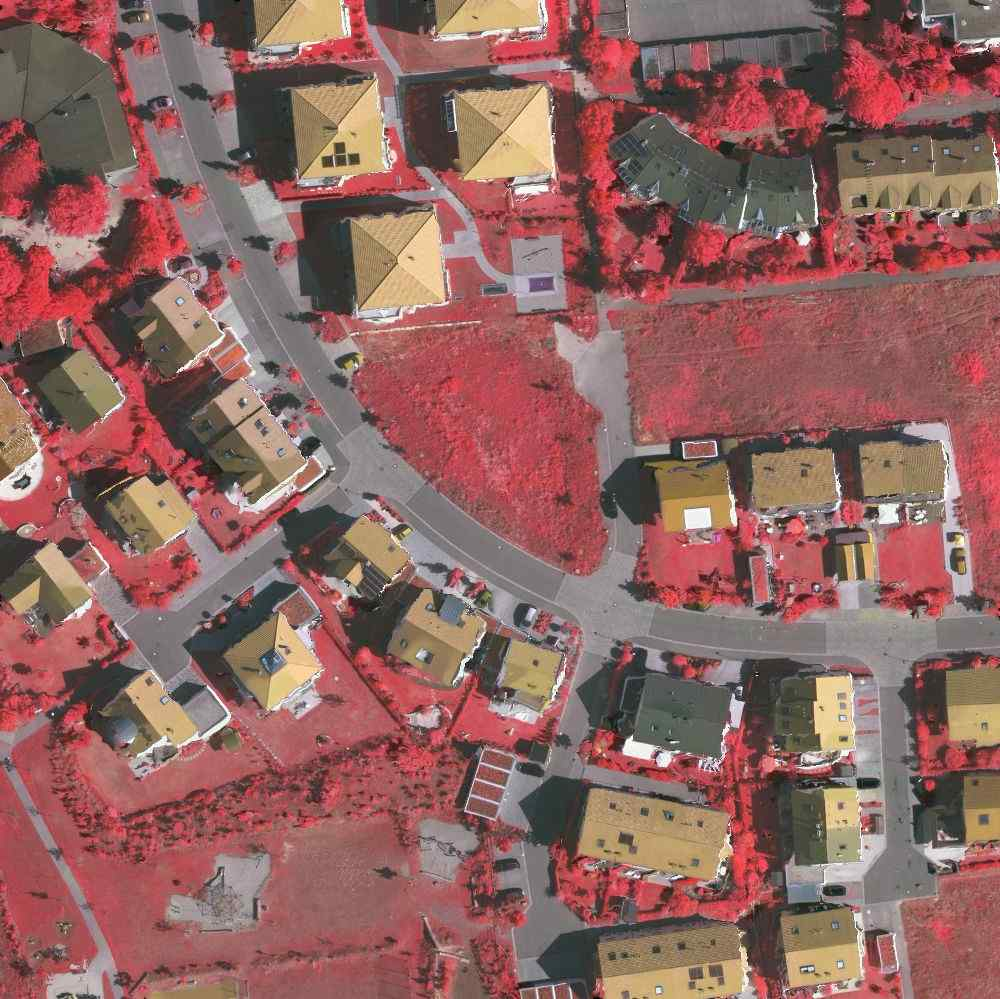
\includegraphics[width=\linewidth]{vaihingen_irrg_37}
    \caption{Image \gls{IRRV}}
    \end{subfigure}
    \hfill
    \begin{subfigure}{0.48\textwidth}
    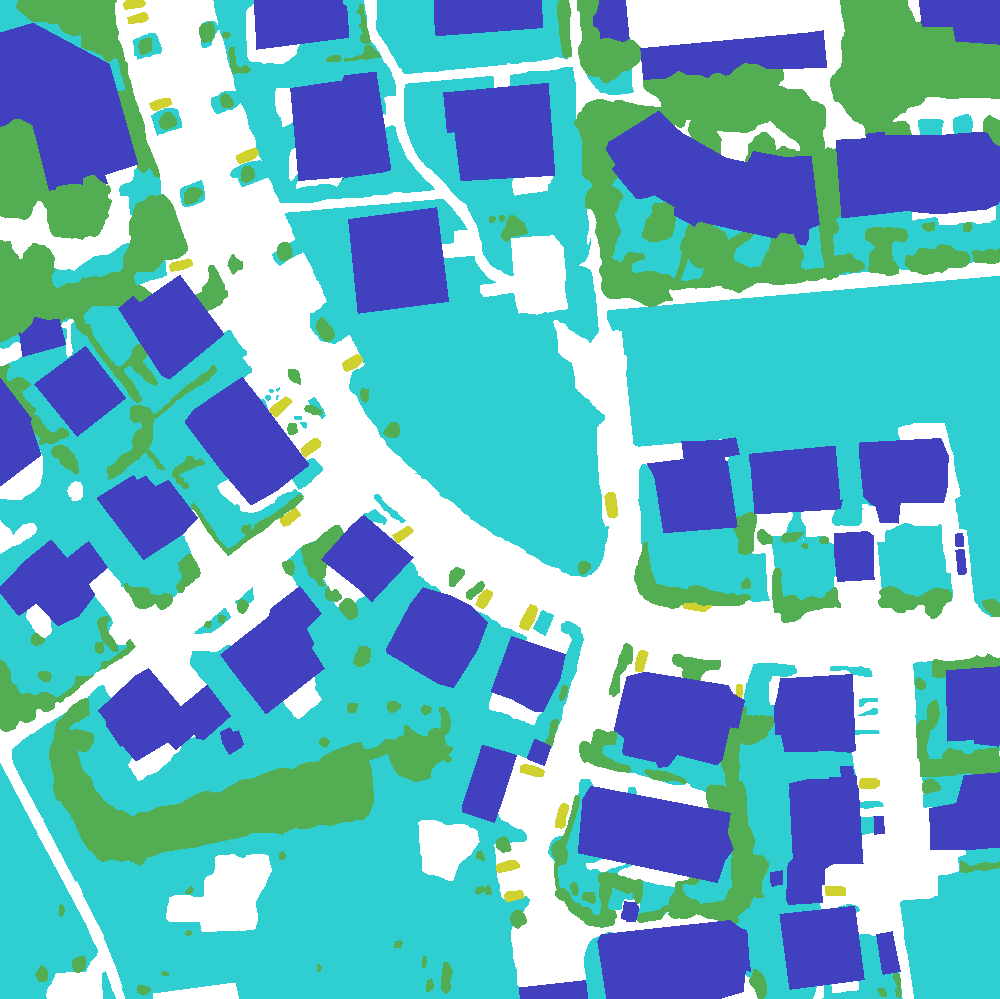
\includegraphics[width=\linewidth]{vaihingen_gt_37}
    \caption{Vérité terrain}
    \end{subfigure}
    \hfill

    \hfill
    \begin{subfigure}{0.48\textwidth}
    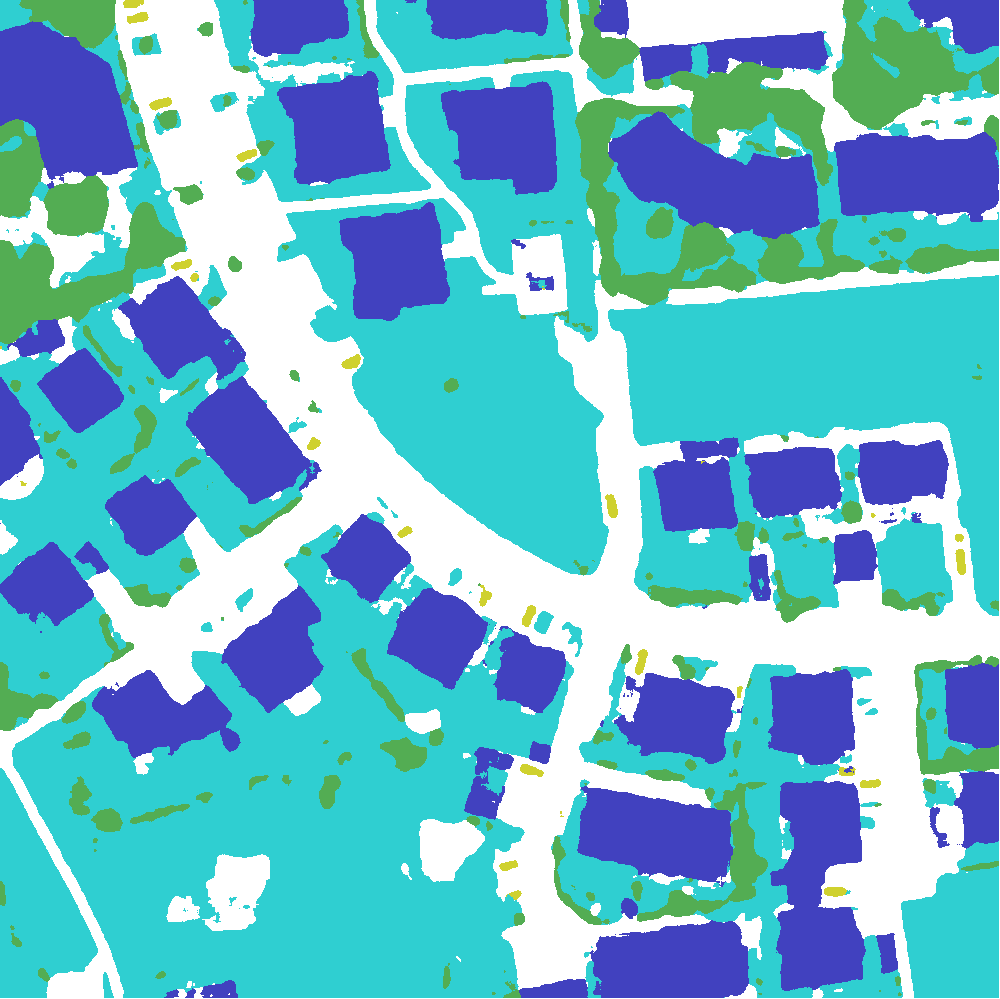
\includegraphics[width=\linewidth]{segnet_irrg_37}
    \caption{SegNet}
    \end{subfigure}
    \hfill
    \begin{subfigure}{0.48\textwidth}
    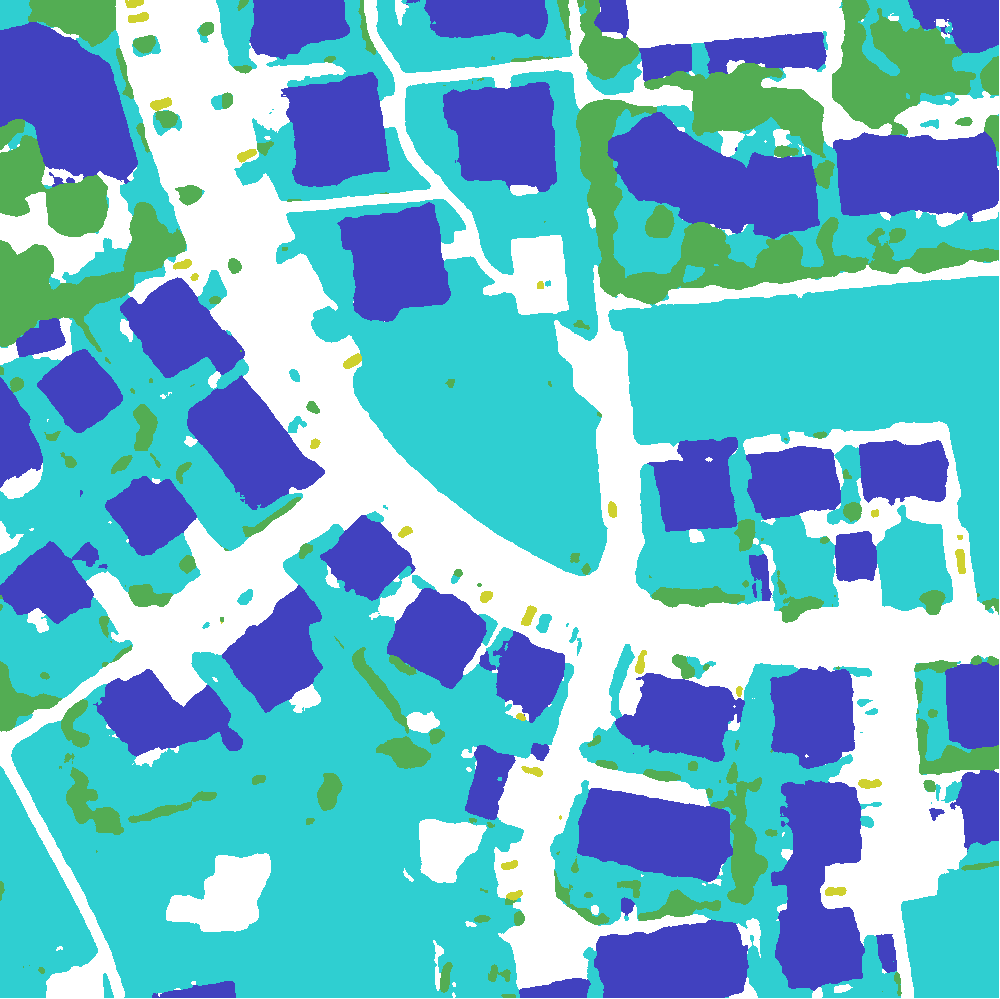
\includegraphics[width=\linewidth]{segnet_irrg_msc_37}
    \caption{SegNet multi-échelles (3 branches)}
    \end{subfigure}
    \hfill
    \caption{Effet de la supervision multi-échelles sur un extrait du jeu de données \gls{ISPRS} Vaihingen. Les petits objets et les surfaces au contexte spatial ambigu bénéficient de la combinaison des prédictions à plusieurs échelles.\\
		\isprslegende}
    \label{fig:vaihingen_images}
\end{figure}

\begin{table}
    \caption{Résultats de validation multi-échelles sur le jeu de données \gls{ISPRS} Vaihingen.}
    \label{tab:dsn_vaihingen}
	\begin{tabularx}{\textwidth}{Y c c c c c c}
    \toprule
    Nombre de branches & Routes & Bâtiments & Vég. basse & Arbres & Véhicules & Exactitude\\
    \midrule
    Pas de branche & 92,2 & 95,5 & \textbf{82,6} & \textbf{88,1} & 88,2 & 90,2 {\small $\pm$ 1,4}\\
    1 branche & 92,4 & 95.7 & 82,3 & 87,9 & \textbf{88,5} & 90,3 {\small $\pm$ 1,5}\\
    2 branches & 92,5 & \textbf{95,8} & 82,4 & 87,8 & 87.6 & 90,3 {\small $\pm$ 1,4}\\
    3 branches & \textbf{92,7} & \textbf{95,8} & \textbf{82,6} & \textbf{88.1} & 88,1 & \textbf{90,5} {\small $\pm$ 1,5}\\
    \bottomrule
    \end{tabularx}
\end{table}

Comme détaillé dans le~\cref{tab:dsn_vaihingen}, la supervision profonde multi-échelles sur SegNet apporte un gain léger, toutefois avec un surcoût calculatoire quasiment nul. Comme attendu, les grandes structures bénéficient le plus des prédictions à faible échelle tandis que les voitures, les plus petits objets d'intérêt du jeu de données, sont plus difficiles à détecter à basse résolution. En outre, il semble que l'absence de structure dans la végétation induit également une confusion entre les arbres et la végétation basse aux échelles inférieures. Augmenter le nombre de branches n'augmente que marginalement les performances du SegNet ce qui indique que la supervision profonde ne joue qu'un rôle limité par rapport à la fusion multi-échelles.

Bien que le gain quantitatif soit faible, une analyse visuelle des cartes obtenues après inférence montre que les améliorations qualitatives ne sont pas négligeables. Comme illustré dans la~\cref{fig:vaihingen_images}, la prédiction multi-échelle permet de régulariser les prédictions et de réduire le bruit qui s'y trouve. Cela simplifie le traitement des cartes \emph{a posteriori}, qu'il s'agisse de leur interprétation par un humain ou d'une vectorisation automatique. Ces résultats sont adéquation avec les travaux postérieurs de~\citet{jiang_rednet_2018} pour la segmentation sémantique d'images \gls{RGB-D}.

En outre, cette étude a également mis en avant que les cartes d'activation intermédiaires du décodeur sont quasiment aussi précises que les cartes à pleine résolution. Par exemple, la carte issue du deuxième bloc convolutif, c'est-à-dire à résolution $1:8$ par rapport à l'image initiale, est seulement 0,5\% moins exacte que celle à résolution $1:1$, l'essentiel des différences provenant de la classe ``véhicule''. Ceci était prévisible dans la mesure où les véhicules ne couvrent qu'environ \SI{30}{\px} en longueur à \SI{9}{\centi\meter/\px}, soit 3-\SI{4}{\px} à résolution $1:8$. Toutefois, les bonnes performances obtenues en utilisant uniquement les prédictions réduites indique qu'il serait possible de se limiter à un décodeur extrêmement simple comprenant uniquement un ou deux blocs convolutifs en décodeur en perdant peu de précision, soit une réduction du nombre de paramètres et du temps de calcul de SegNet d'environ 30\%. Cette méthode pourrait permettre de réduire le temps d'inférence lorsque la détection des petits objets n'est pas au c\oe{}ur du problème.

\paragraph{Convolution multi-kernel}
\begin{figure}[h]
  %\centering
  \captionsetup[subfigure]{singlelinecheck=off,justification=centering}
  \captionsetup[subfigure]{labelformat=empty}
  \begin{subfigure}[t]{0.125\textwidth}
    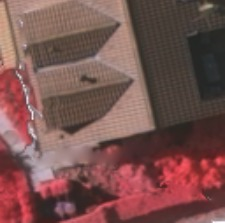
\includegraphics[width=\textwidth]{158_irrg}
    \caption{\gls{IRRV}}
  \end{subfigure}%
  \begin{subfigure}[t]{0.125\textwidth}
    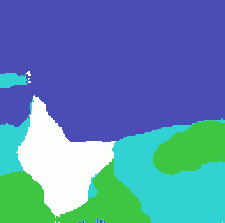
\includegraphics[width=\textwidth]{158_pred_irrg}
    \caption{Prédiction}
  \end{subfigure}%
  \begin{subfigure}[t]{0.125\textwidth}
    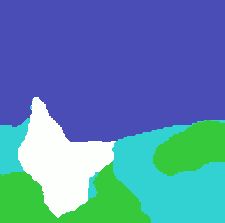
\includegraphics[width=\textwidth]{158_pred_irrg_context}
    \caption{Prédiction (multi)}
  \end{subfigure}%
  \begin{subfigure}[t]{0.125\textwidth}
    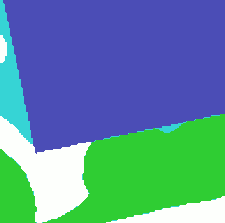
\includegraphics[width=\textwidth]{158_gt}
    \caption{Vérité terrain}
  \end{subfigure}%
	\begin{subfigure}[t]{0.125\textwidth}
		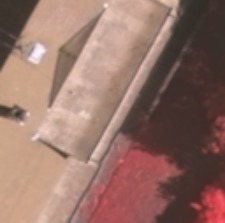
\includegraphics[width=\textwidth]{300_irrg}
		\caption{\gls{IRRV}}
	\end{subfigure}%
	\begin{subfigure}[t]{0.125\textwidth}
		
\includegraphics[width=\textwidth]{300_pred_irrg}
		\caption{Prédiction}
	\end{subfigure}%
	\begin{subfigure}[t]{0.125\textwidth}
		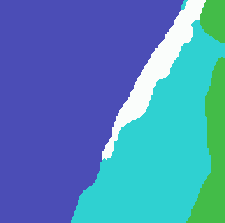
\includegraphics[width=\textwidth]{300_pred_irrg_context}
		\caption{Prédiction (multi)}
	\end{subfigure}%
	\begin{subfigure}[t]{0.125\textwidth}
		
\includegraphics[width=\textwidth]{300_gt}
		\caption{Vérité terrain}
	\end{subfigure}
  \caption{Effets de la couche convolutive multi-kernel sur des extraits du jeu de données \gls{ISPRS} Vaihingen.\\
	\isprslegende}
  \label{fig:patches_context}
\end{figure}

Comme indiqué dans le~\cref{tab:vaihingen_stride}, l'utilisation d'une dernière couche convolutive multi-kernel permet de gagner 0,4\% d'exactitude supplémentaire. Ce gain accompagne un lissage des cartes prédites permettant de faire disparaître certains artefacts de classification sous forme de bruit poivre et sel, comme illustré dans la~\cref{fig:patches_context}.
\citet{brahimi_multiscale_2018} ont par la suite rapporté des résultats similaires en utilisant avec succès la convolution multi-kernel sur des modèles DenseNet appliqués à la segmentation sémantique d'images de conduite autonome.

\subsubsection{Résultats finaux}

\begin{table}[t]
  \centering
  \caption{Résultats du \gls{ISPRS} 2D Semantic Labeling Challenge Vaihingen.}
  \rowcolors{2}{gray!15}{white}
  \begin{tabularx}{\textwidth}{ Y c c c c c c }
  \toprule
  Méthode & Routes & Bâtiments & Vég. basse & Arbres & Véhicules & Exactitude\\
  \midrule
  Stair Vision Library {\scriptsize (``SVL\_3'')}\cite{gerke_use_2015} & 86,6\% &	91,0\% &	77,0\% &	85,0\%	& 55,6\% &	84,8\% \\
  RF + CRF {\scriptsize (``HUST'')}\cite{quang_efficient_2015} & 86,9\% & 92,0\% &	78,3\% &	86,9\% &	29,0\% &	85,9\% \\
  Ensemble de CNN {\scriptsize (``ONE\_5'')}\cite{boulch_dag_2015} & 87,8\% &	92,0\% &	77,8\% &	86,2\% &	50,7\% &	85,9\% \\
  FCN {\scriptsize (``UZ\_1'')}\cite{volpi_dense_2017} & 89,2\% &	92,5\% &	81,6\% &	86,9\% &	57,3\% &	87,3\% \\
  FCN {\scriptsize (``UOA'')}\cite{lin_efficient_2015} & 89,8\% &	92,1\% &	80,4\% &	88,2\% &	82,0\% &	87,6\% \\
  CNN + RF + CRF {\scriptsize (``ADL\_3'')}\cite{paisitkriangkrai_effective_2015} & 89,5\% &	93,2\% &	82,3\% &	88,2\% &	63,3\% &	88,0\% \\
  FCN {\scriptsize (``DLR\_2'')}\cite{marmanis_semantic_2016} & 90,3\% &	92,3\% &	82,5\% &	89,5\% &	76,3\% &	88,5\% \\
  FCN + RF + CRF {\scriptsize (``DST\_2'')}\cite{sherrah_fully_2016} & 90,5\% &	93,7\% &	83,4\% &	89,2\% &	72,6\% &	89,1\% \\
  %FCN + CRF + frontières {\scriptsize (``DLR\_10'')}\cite{marmanis_classification_2017} & 92.3\% & 95.2\% & 84.1\% & 90.0\% & 79.3\% & 90.3\%\\
  \midrule
  \textbf{SegNet++} (multi-kernel)\cite{audebert_semantic_2016} & \textbf{91,5}\% &	94,3\% &	82,7\% &	89,3\% &	\textbf{85,7}\% &	89,4\% \\
  %\textbf{SegNet++} (multi-kernel + fusion) & 91,0\% &	\textbf{94,5}\% &	\textbf{84,4}\% &	\textbf{89,9}\% &	77,8\% &	\textbf{89,8}\% \\
  \bottomrule
  \end{tabularx}
  \label{tab:final_vaihingen}
\end{table}

\begin{table}[t]
    \caption{Résultats du \gls{ISPRS} 2D Semantic Labeling Challenge Potsdam.}
    \label{table:final_potsdam}
    \setlength\tabcolsep{4pt}
	\begin{tabularx}{\textwidth}{Y c c c c c c}
    \toprule
	Method & Routes & Bâtiments & Vég. basse & Arbres & Véhicules & Exactitude\\
    \midrule
    FCN + CRF + caractéristiques expertes~\cite{liu_dense_2017} & 91.2 & 94.6 & 85.1 & 85.1 & 92.8 & 88.4\\
    FCN~\cite{sherrah_fully_2016} & 92.5 & \textbf{96.4} & 86.7 & 88.0 & 94.7 & 90.3\\
    \midrule
    SegNet (IRRG) & 92.4 & 95.8 & 86.7 & 87.4 & 95.1 & 90.0\\
    \bottomrule
    \end{tabularx}
\end{table}

\begin{figure}[h]
  \begin{subfigure}[t]{0.25\textwidth}
    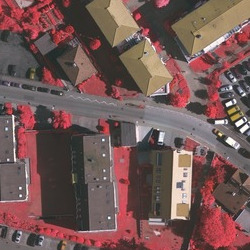
\includegraphics[width=\textwidth]{top}
    \caption{Image \gls{IRRV}}
  \end{subfigure}%
  % \begin{subfigure}[t]{0.19\textwidth}
  %     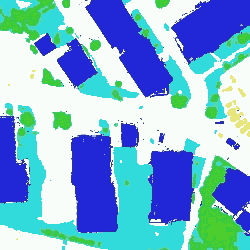
\includegraphics[width=\textwidth]{svl}
  %     \caption{``SVL''\cite{gerke_use_2015}}
  %   \end{subfigure}
  \begin{subfigure}[t]{0.25\textwidth}
    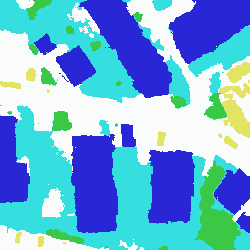
\includegraphics[width=\textwidth]{rf}
    \caption{RF + \glsname{CRF}~\cite{quang_efficient_2015}}
  \end{subfigure}%
  \begin{subfigure}[t]{0.25\textwidth}
    \includegraphics[width=\textwidth]{fcn}
    \caption{``DLR'' (\gls{FCN})~\cite{marmanis_semantic_2016}}
  \end{subfigure}%
    \begin{subfigure}[t]{0.25\textwidth}
    \includegraphics[width=\textwidth]{segnet}
    \caption{\textbf{SegNet++}}
  \end{subfigure}
  \caption{Comparaison des segmentations obtenues sur un extrait du jeu de test \gls{ISPRS} Vaihingen.\\
  \isprslegende}
  \label{fig_segnet_qualitative}
\end{figure}

\begin{figure}[h]
	\centering
	\foreach\picname\picpath\w in {Image \gls{RVB}/potsdam_rgb_3_11/0.48,Vérité terrain/potsdam_gt_3_11/0.48,Prédiction (SegNet)/segnet_irrg_potsdam_3_11/0.9}{%
	\begin{subfigure}{\w\textwidth}
		\includegraphics[width=\textwidth]{\picpath}
		\caption*{\picname}
	\end{subfigure}
	}
	\caption{Exemple de segmentation obtenue par SegNet sur le jeu de données \gls{ISPRS} Potsdam (tuile 3\_11).\\\isprslegende}
	\label{fig:potsdam_images}
\end{figure}

Notre meilleur modèle améliore l'état-de-l'art sur le jeu de données \gls{ISPRS} Vaihingen (cf. \cref{tab:final_vaihingen}) \footnote{Résultats détaillés : \url{http://www2.\gls{ISPRS}.org/vaihingen-2d-semantic-labeling-contest.html}}. La \cref{fig_segnet_qualitative} illustre une comparaison qualitative entre différentes méthodes. Les métriques sont calculées en ignorant un rayon de $3$ pixels autour des bordures afin de tenir compte d'éventuelles imprécisions dans la vérité terrain.

Au moment de la soumission de ces résultats, la meilleure méthode de l'état de l'art utilisait une combinaison de \gls{FCN} et de caractéristiques expertes, tandis que la nôtre n'utilise que l'apprentissage statistique. La meilleure méthode précédente utilisant uniquement un \gls{FCN} (``DLR\_1'') atteint 88,4\%, ce que nous améliorons de 1\%. Les précédentes méthodes utilisant les \gls{CNN} atteignent 85,9\% (``ONE\_5''\cite{boulch_dag_2015}) et 86,1\% (``ADL\_1''\cite{paisitkriangkrai_effective_2015}). Notre méthode obtient des résultats supérieurs, sans recourir à des caractéristiques expertes ou à des post-traitement structurés comme les \gls{CRF}.

Sur le jeu de données \gls{ISPRS} Potsdam (cf. \cref{table:final_potsdam}), notre méthode est compétitive avec l'état de l'art au moment de la soumission. Notamment, nous améliorons l'état de l'art sur les méthodes n'utilisant que la donnée optique de 0,3\% par rapport au \gls{FCN} de \citet{sherrah_fully_2016} et de 4,2\% par rapport au \gls{FCN} de~\citet{volpi_dense_2017}. Un exemple d'image complète segmentée est donné dans la~\cref{fig:potsdam_images}.

\begin{figure}[h]
	\captionsetup[subfigure]{singlelinecheck=off,justification=centering}
	\begin{subfigure}{0.5\textwidth}
		\begin{subfigure}[t]{0.3\textwidth}
	    	\includegraphics[width=\textwidth]{error_top}
	        \caption*{Image \gls{IRRV}}
	    \end{subfigure}
	    \begin{subfigure}[t]{0.3\textwidth}
	    	\includegraphics[width=\textwidth]{error_gt}
	        \caption*{Vérité terrain}
	    \end{subfigure}
	    \begin{subfigure}[t]{0.3\textwidth}
	    	\includegraphics[width=\textwidth]{error_pred}
	        \caption*{Prédiction}
	    \end{subfigure}
	    \caption{Les cartes produites par SegNet sont parfois plus précises que la vérité terrain.}
	    \label{fig:unprecise_transition}
	\end{subfigure}
	\begin{subfigure}{0.5\textwidth}
		\begin{subfigure}[t]{0.3\textwidth}
	    	\includegraphics[width=\textwidth]{geometric_dist_top}
	        \caption*{Image \gls{IRRV}}
	    \end{subfigure}
	    \begin{subfigure}[t]{0.3\textwidth}
	    	\includegraphics[width=\textwidth]{geometric_dist_gt}
	        \caption*{Vérité terrain}
	    \end{subfigure}
	    \begin{subfigure}[t]{0.3\textwidth}
	    	\includegraphics[width=\textwidth]{geometric_dist_pred}
	        \caption*{Prédiction}
	    \end{subfigure}
	    \caption{SegNet est susceptible de surapprendre sur des déformations géométriques dues à des erreurs d'ortho-rectification.}
	    \label{fig:geometric_dist}
	\end{subfigure}
	\caption{Cas limites de désaccord entre les prédictions faites par SegNet et la vérité terrain.\\
	\isprslegende}
\end{figure}

Il est intéressant de constater que les performances des modèles sont telles que certaines erreurs deviennent attribuables aux ambiguïtés des annotations. La~\cref{fig:unprecise_transition} illustre ainsi un cas où la vérité terrain ne suit pas parfaitement les contours de l'arbre, tandis que le modèle s'avère très fidèle. En outre, le processus d'ortho-rectification de la mosaïque d'images a introduit des distorsions géométriques qui ne sont pas prises en compte dans la vérité terrain, créant un désaccord entre la l'apparence visuelle des pixels et la sémantique qui leur est attribuée, comme le montre la~\cref{fig:geometric_dist}. Ces erreurs montrent par ailleurs qu'il devient difficile de faire progresser significativement les performances des modèles, tant les résultats obtenus par les \gls{FCN} sont proches de ce qui est raisonablement attendu par les organisateurs du \gls{ISPRS} 2D \emph{Semantic Labeling Benchmark}.

En conclusion, nous avons démontré que les \gls{FCN} se prêtent particulièrement bien à la segmentation sémantique d'images aériennes. En particulier, sur la base de données \gls{ISPRS}, nous avons pu montrer d'une part la nette supériorité des réseaux entièrement convolutifs par rapport aux approches de l'état de l'art en classification par région. En outre, nous avons proposé plusieurs bonnes pratiques concernant l'initialisation de ces réseaux et le paramétrage des fenêtres glissantes pour le traitement des images aériennes. Enfin, nous avons proposé deux méthodes de segmentation permettant d'inclure différentes échelles et contextes spatiaux au sein du réseau. Ces approches nous ont permis de faire progresser l'état de l'art. Toutefois, ces succès restent encore limités au domaine de l'imagerie 3 canaux \gls{IRRV} et \gls{RVB} à très haute résolution. Le chapitre suivant s'intéresse à étendre ces résultats sur d'autres capteurs couramment utilisés en observation de la Terre.

%\bibliographystyle{plainnat}
%\bibliography{Chapitre2/Biblio}
\printbibliography
